% Preamble

%% Document type
\documentclass[
	12pt,
	twoside
]{book}

%% Layout
%\usepackage[
%	a4paper,
%	top=2cm,
%	bottom=2cm,
%	left=3cm,
%	right=3cm,
%]{geometry}

%% Layout (simplified)
\usepackage[
	a4paper,
	vmargin=2cm,
	hmargin=3cm
]{geometry}
\usepackage{pdflscape}

%% Line spacing, paragraph spacing and indentation
\renewcommand{\baselinestretch}{1.15}
\setlength{\parskip}{6pt}
\setlength{\parindent}{0pt}

%% Character encoding
\usepackage[utf8]{inputenc}

%% Font
\usepackage[T1]{fontenc}

%% Languaje
\usepackage[english]{babel}

%% Links
\usepackage[
	colorlinks=true,
	linkcolor=blue,
	urlcolor=blue
	%allcolors=blue
]{hyperref}

%% Tables
\usepackage{longtable}
\usepackage{multirow}

%% Long lists
\usepackage{enumitem}
\newlist{longitem}{itemize}{10}
\setlist[longitem, 1]{label=$\bullet$)}
\setlist[longitem, 2]{label=$-$)}
\setlist[longitem, 3]{label=$*$)}
\setlist[longitem, 4]{label=$\circ$)}
\setlist[longitem, 5]{label=$\blacksquare$)}
\setlist[longitem, 6]{label=$\blacktriangleright$)}
\setlist[longitem, 7]{label=$\blacklozenge$)}
\setlist[longitem, 8]{label=$\lozenge$)}
\setlist[longitem, 9]{label=$\otimes$)}
\setlist[longitem, 10]{label=$\bigodot$)}

%% Floating figures
\usepackage{float}

%% Color settings
\usepackage[table]{xcolor}
\usepackage[table]{xcolor}
\definecolor{azulUC3M}{RGB}{0,0,102}
\definecolor{gray97}{gray}{.97}
\definecolor{gray75}{gray}{.75}
\definecolor{gray45}{gray}{.45}

%% Head and foot
\usepackage{fancyhdr}
\pagestyle{fancy}
\fancyhead{}
\fancyhead[LE]{Telecommunication Systems}
\fancyhead[CE]{}
\fancyhead[RE]{Universidad Carlos III de Madrid}
\fancyhead[LO]{Universidad Carlos III de Madrid}
\fancyhead[CO]{}
\fancyhead[RO]{Telecommunication Systems}
\fancyfoot{}
\fancyfoot[LE]{}
\fancyfoot[CE]{\thepage}
\fancyfoot[RE]{}
\fancyfoot[LO]{}
\fancyfoot[CO]{\thepage}
\fancyfoot[RO]{}
\renewcommand{\headrulewidth}{1pt}
\renewcommand{\footrulewidth}{0pt}
%\renewcommand{\headruleskip}{1pt}
%\renewcommand{\footruleskip}{1pt}

%% Code blocks
\usepackage{listings}
\usepackage{lstautogobble}
\lstdefinestyle{mystyle}{
	basicstyle=\footnotesize\ttfamily,
	breakatwhitespace=false,
	breaklines=true,
	captionpos=b,
	keepspaces=true,
	showspaces=false,
	showstringspaces=false,
	showtabs=false,
	tabsize=4
}
\lstset{
	style=mystyle,
	language=tex,
	autogobble=true
}

%% Math expressions
\usepackage{amsmath, amssymb, amsfonts, amsthm}

%% Images
\usepackage{graphicx}
\usepackage{tikz}
\usepackage{plantuml}

%% Document information
\title{Telecommunication Systems}
\author{Universidad Carlos III de Madrid}
\date{Updated: \today}



\begin{document}



\begin{titlepage}
	\begin{sffamily}
	\color{azulUC3M}

	\begin{center}

		% Logotipo de la Universidad
		\begin{figure}[H]
			\makebox[\textwidth][c]{
\includegraphics[width=16cm]{Imágenes/UC3M/Portada_Logo.png}}
		\end{figure}

		\vspace{2.5cm}

		\begin{Large}
			Bachelor in Telecommunication Technologies Engineering\\			
			%Academic Year (e.g. 2016-2017)\\
			%\vspace{2cm}		
			%\textsl{Bachelor Thesis}
			\bigskip
		\end{Large}

		 	{\Huge Telecommunication Systems}\\
		 	\vspace*{0.5cm}
	 		\rule{10.5cm}{0.1mm}\\
			\vspace*{0.9cm}
			{\LARGE Juan Manuel Espinosa Moral}\\ 
			\vspace*{1cm}

		\begin{Large}
			Víctor Pedro\\
			Gil Jiménez\\
			Leganés, \today\\
		\end{Large}
	\end{center}

	\vfill

	\color{black}

	% Licencia Creative Commons
	
\includegraphics[width=4.2cm]{Imágenes/UC3M/creativecommons.png}\\
	This work is licensed under Creative Commons \textbf{Attribution – Non Commercial – Non Derivatives}

	\end{sffamily}
\end{titlepage}

\newpage

%\maketitle

\tableofcontents

\chapter{Introduction to telecommunication systems}

\section{Basic concepts}

\subsection{Definition}

According to ITU, telecommunication is any transmission, emission or reception of signs, signals, writings, images and sounds or intelligence of any nature by wire, radio, optical or other electromagnetic systems. Then, a telecommunication system is a bounded technological gadget to provide this service.

\subsection{Characterization}

A telecommunication system can be characterized by the following parameters:

\begin{itemize}
	\item Transmission quality, usually using objective measurements like probability of error ($P_e$) and signal-to-noise ratio ($SNR$), but also using subjective criteria.
	\item Delay in propagation or network access.
	\item Availability in time and location.
\end{itemize}

\subsection{Telecommunication systems architecture}

Telecommunication systems are implemented through networks and terminals.

In order to describe telecommunication systems, we define two elements:

\begin{itemize}
	\item Functional entity: Set of functions in the network with common goal. It might be a physical equipment or not.
	\item Reference points (interfaces): Connections between functional entities.
\end{itemize}

\begin{figure}[H]
	\centering
	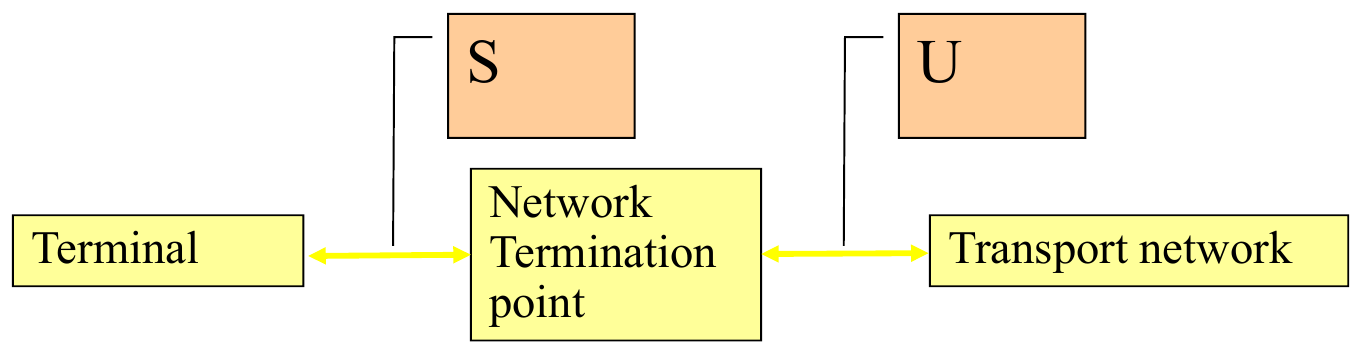
\includegraphics[
		width=14cm,
		%height=15cm
	]{Imágenes/Tema 1/Architecture.png}
	\caption{
		\label{fig:unit1_arch}
		Telecommunication systems architecture
	}
\end{figure}

\subsection{Communications networks}

A network is a set of organized resources both logical and physical for allowing the telecommunication. To accomplish with that purpose, the carry out:

\begin{itemize}
	\item Transmission and reception.
	\item Switching.
	\item Signaling.
\end{itemize}

The network is a limited resource and it must be shared, for which networks implement two strategies:

\begin{itemize}
	\item {
		Multiplexing

		\begin{figure}[H]
			\centering
			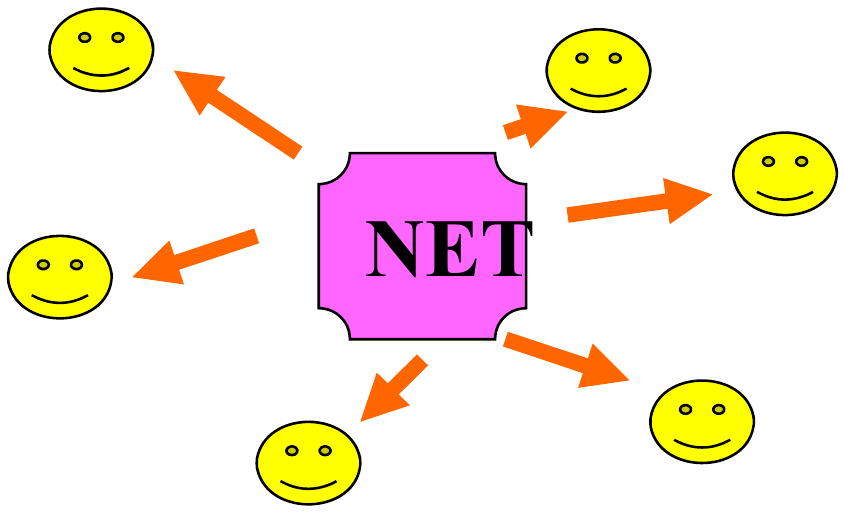
\includegraphics[
				%width=14cm,
				height=3cm
			]{Imágenes/Tema 1/Multiplexation.png}
			\caption{
				\label{fig:unit1_muiltiplexation}
				Multiplexing
			}
		\end{figure}
	}
	\item {
		Multiple access

		\begin{figure}[H]
			\centering
			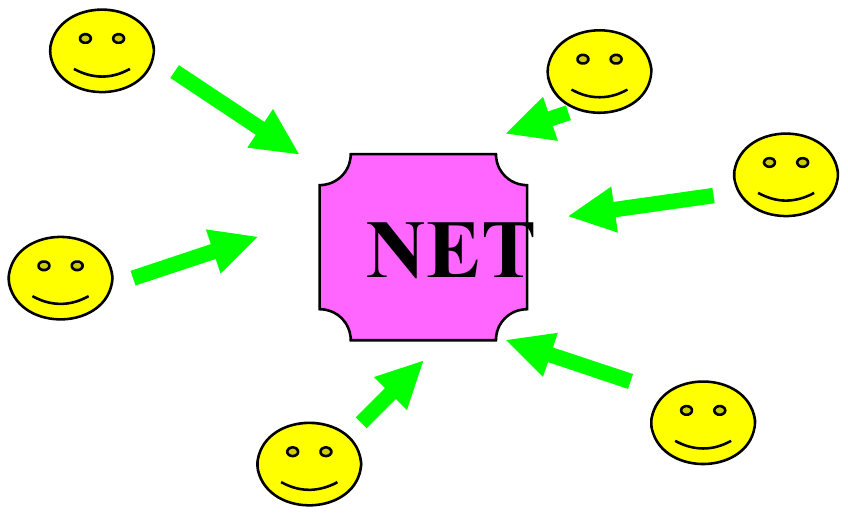
\includegraphics[
				%width=14cm,
				height=3cm
			]{Imágenes/Tema 1/Multiple access.png}
			\caption{
				\label{fig:unit1_multiple}
				Multiple access
			}
		\end{figure}
	}
\end{itemize}

Althought many communications networks can perform both broadcasting and switching, due to specialization, they can be classified in these categories:

\begin{itemize}
	\item {
		Broadcast networks: Their purpose is distributing information from a transmitter to a wide number of users, so the transmitter sends the information to the shared medium from which users can access to data. Each terminal selects information addressed to it. Some examples are television network and Local Area Networks (LAN).

		\begin{figure}[H]
			\centering
			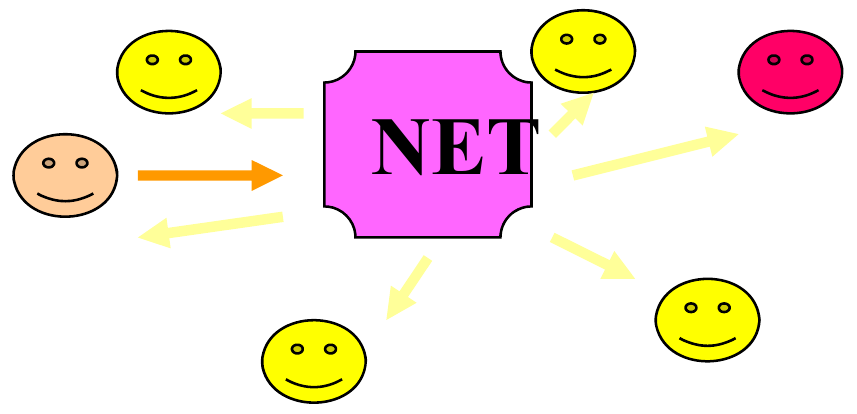
\includegraphics[
				%width=14cm,
				height=3cm
			]{Imágenes/Tema 1/Broadcasting.png}
			\caption{
				\label{fig:unit1_broadcast}
				Broadcast networks
			}
		\end{figure}
	}
	\item {
		Switching networks: Their purpose is being specific with source and destination, usually the source terminal selects the destination. The network must establish a physical channel between both terminals. An example is Plain Old Telephony Service (POTS).

		\begin{figure}[H]
			\centering
			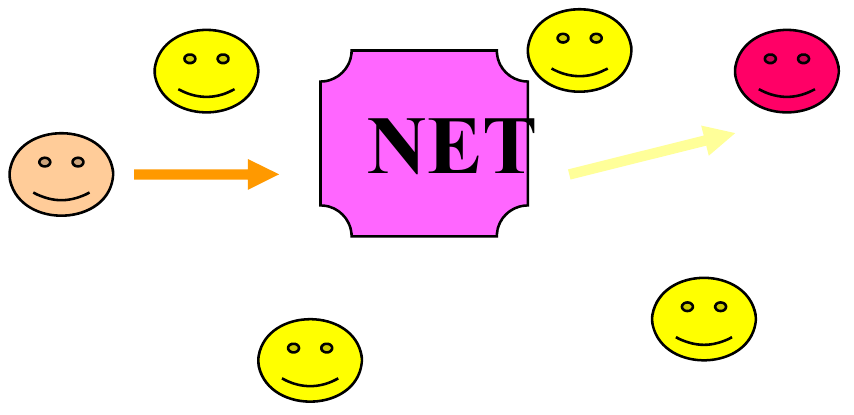
\includegraphics[
				%width=14cm,
				height=3cm
			]{Imágenes/Tema 1/Switching.png}
			\caption{
				\label{fig:unit1_switching}
				Switching networks
			}
		\end{figure}
	}
\end{itemize}

\subsection{Telecommunication services}

A service is a set of logical and physical wherewithal operated and managed by the service provider to serve the client and a set of rules for usage and access. All together satisfy the telecommunication required by users.

Services can be classified in many ways:

\begin{itemize}
	\item {
		In function of their complexity:
		\begin{itemize}
			\item Basic services: They exist by their own, like the basic telephony service.
			\item Suplementary services: They are associated to a basic service. Some examples are Calling Line Identification, waiting call, Explicit Call Transfer, Call Hold, multiparty service, etc.
		\end{itemize}
	}
	\item {
		According to ITU-CCITT:
		\begin{itemize}
			\item Bearer services: They provide the transport capacity.
			\item Teleservices or end services: They provide complete communication capacity. They include terminals even it hey are not provided by the service provider. They include added value services like storage or processing.
		\end{itemize}
		\begin{figure}[H]
			\centering
			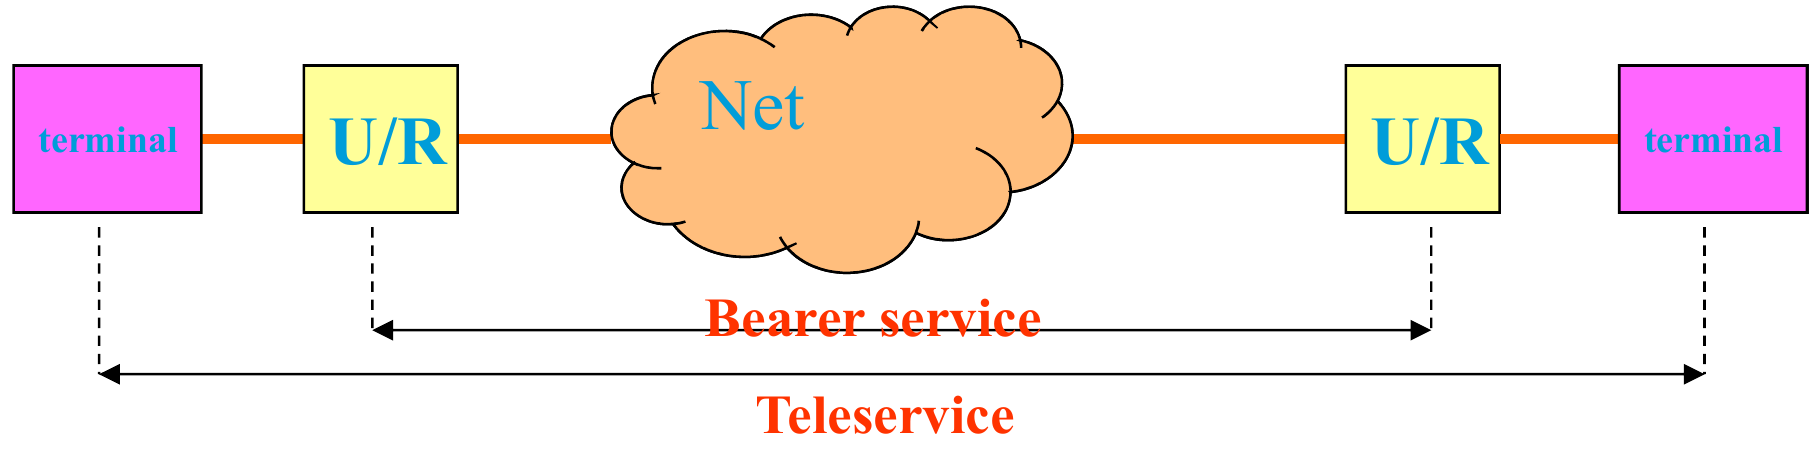
\includegraphics[
				width=14cm,
				%height=15cm
			]{Imágenes/Tema 1/Classification according to ITU-CCITT.png}
			\caption{
				\label{fig:unit1_according}
				Classification according to ITU-CCITT
			}
		\end{figure}
	}
	\item {
		Other classifications:

		\begin{itemize}
			\item Users' groups: intercommunication, social communications, commercial, residential, ...
			\item Type of information: voice, data, text, control, telemetry, ...
			\item {
				Capacity: wideband, narrowband, ...

				\begin{figure}[H]
					\centering
					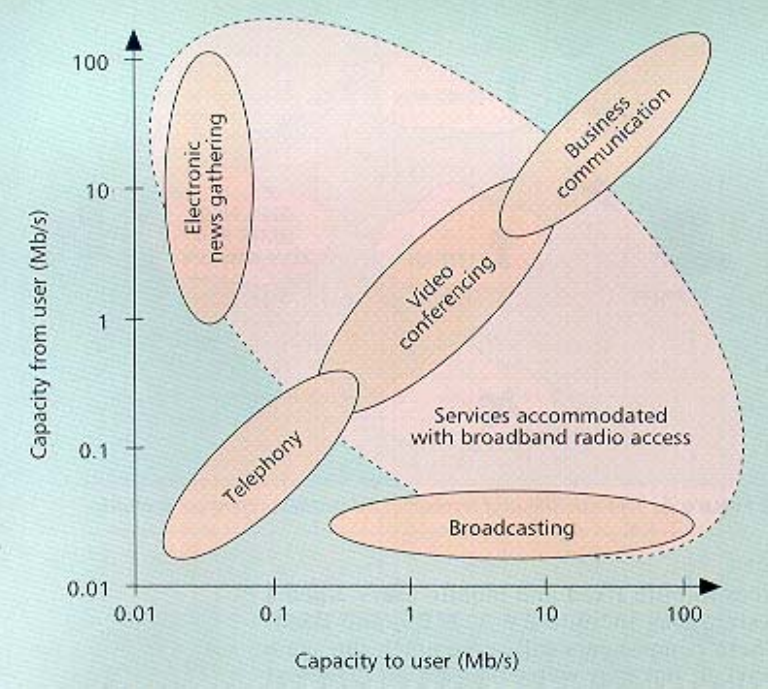
\includegraphics[
						width=14cm,
						%height=15cm
					]{Imágenes/Tema 1/Classification in function of capacity.png}
					\caption{
						\label{fig:unit1_capacity}
						Classification in function of capacity
					}
				\end{figure}
			}
			\item Type of communication: query, broadcast, conversation, messages, symmetric, asymmetric, ...
			\item {
				Mobility: fixed, portable, mobile, ...

				\begin{figure}[H]
					\centering
					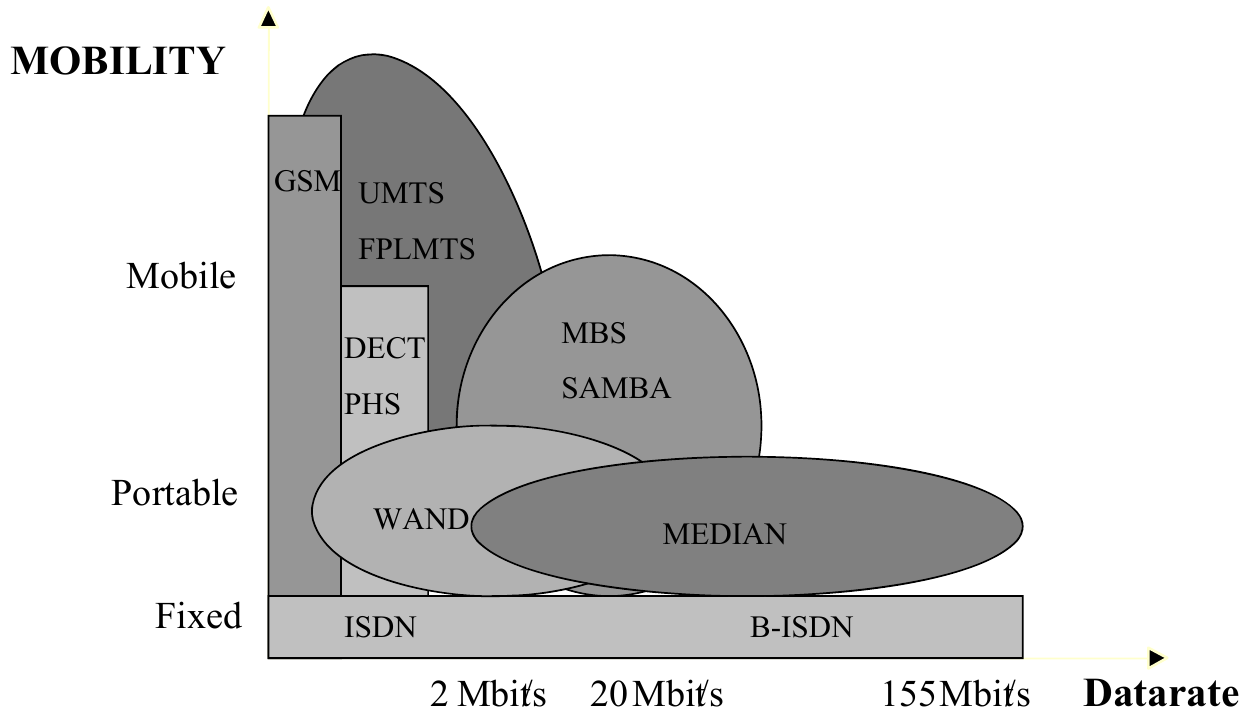
\includegraphics[
						width=13cm,
						%height=15cm
					]{Imágenes/Tema 1/Classification in function of mobility.png}
					\caption{
						\label{fig:unit1_mobility}
						Classification in function of mobility
					}
				\end{figure}
			}
			\item Type of network: POTS, ISDN, radio, ...
		\end{itemize}
	}
\end{itemize}

For further study, the main services to consider are:

\begin{itemize}
	\item Telephony service: Their purpose is voice transmission among users. It is high demanded and the most representative. Around it, new services are included, like digitality and mobility, ...
	\item Data transfer service: Their purpose is digital data transmission. It is supported by POTS or specific data networks
	\item Added value services: fax, dataphone, videotex, teletext, ...
	\item Radio communication services: Air is the physical medium to transmit through.
\end{itemize}

\section{Telecommunications regulations}

\subsection{Introduction}

For the propper development of telecommunications, legal and institutional regulations are applied. Their purpose is:

\begin{itemize}
	\item Fair use of electromagnetic spectrum.
	\item Achieve compatibility between telecommunication systems.
	\item Ease the development of economies of scale.
\end{itemize}

\subsection{Spectral regulation}

In wireless communications, electromagnetic spectrum usage must be optimized. This purpose is carried out through the following processes:

\begin{itemize}
	\item Allocation: Entry in a table of frequency allocations of a \textbf{frequency band} for the \textbf{preferent purpose} of its use by one or more terrestrial service, space radiocommunication service or radioastronomy service under specified conditions. This term shall also be applied to the frequency band concerned, which is refered as allocated band.
	\item Allotment: Entry of a designated \textbf{radio frequency or radio frequency channel} in an agreed plan, adopted by a competent conference for its use by one or more administrations for a terrestrial or space radiocommunication \textbf{preferent service} in one or more identified countries or geographical areas and under specified conditions. This term shall also be applied to the radio frequency or radio frequency channel concerned, which is refered as alloted radio frequency or alloted radio frequency channel.
	\item Assignment: \textbf{Authorization given by an administration for a radio station to use a radio frequency or radio frequency channel} under specified conditions. This term shall also be applied to the radio frequency or radio frequency channel concerned, which is refered as assigned radio frequency or assigned radio frequency channel.
\end{itemize}

\subsection{Organizations for the telecommunication regulation}

For the propper development and application of regulations and common standards, there are specific institutions and associations. Main organizations are:

\begin{itemize}
	\item {
		International Telecommunication Union (ITU): Dependant on United Nations. Its purpose is to \textbf{harmonize} the telecommunication \textbf{worldwide} through cooperation, development and normalization. It is divided into temporal committees, but has some permanent bodies:
		\begin{itemize}
			\item Secretary.
			\item UIT-R: Radiocommunications.
			\item UIT-T: Telegraphy, telephony and telematics.
			\item Frequency register.
		\end{itemize}
	}
	\item International Standardization Organization (ISO): It is an international association of national standards organizations. It \textbf{facts norms} \textbf{worldwide}. Some ISO standards examples are: credit card format, telephony cards, intelligent cards, ISO 9000 (quality management).
	\item World Radio Conference (WRC): It defines \textbf{worldwide} \textbf{frequency bands and services}.
	\item Institute of Electrical and Electronic Engineers (IEEE or IE3): It is an independent organization that developes technology standards. It \textbf{facts norms} \textbf{worldwide}.
	\item Federal Communications Commission (FCC): It is an independent agency of United States government. Its purpose is to \textbf{harmonize} telecommunications in \textbf{USA}.
	\item American National Standards Institute (ANSI): It is a private organization. It \textbf{facts norms} in \textbf{USA}.
	\item European Commission (EC): It is the general chair for information society in European Union. It carries out projects and programs. It is composed by a group of senior officers.
	\item \textit{Conférence européenne des administrations des postes et télécommunications} (\textit{CEPT}, in English, European Conference of Postal and Telecommunications Administrations): It is an association of national telecommunication organizations from Europe. Its purpose is to \textbf{harmonize} the telecommunication worldwide (specially in \textbf{Europe}) through cooperation, development and normalization.
	\item European Telecommunication Standards Institute (ETSI): Dependant on CEPT. Its purpose is providing standards on telecommunication systems (it \textbf{facts norms} for \textbf{Europe}).
	\item \textit{Asociación Española de Normalización} (\textit{UNE}, former \textit{AENOR}, in English, Spanish Association of Standardization and Certification): It \textbf{facts norms} in \textbf{Spain}.
	\item \textit{Cuadro Nacional de Atribución de Frecuencias} (\textit{CNAF}, in English, National Table of Frequency Allocations): \textbf{Frequency assignment} in \textbf{Spain}.
\end{itemize}

\begin{table}
	\centering
	\begin{tabular}{lcccc}
		\hline
		~				& Telecommunications	& Standards	& Radiofrequencies	& Others \\
		\hline
		International	& ITU 					& ISO, IEEE	& WRC				& \\
		USA				& FCC					& ANSI		&					& \\
		Europe			& CEPT					& ETSI		&					& EC \\
		Spain			&						& UNE		& CNAF				& \\
		\hline
	\end{tabular}
	\caption{
		\label{tab:unit1_organizations}
		Organizations for the telecommunication regulation
	}
\end{table}

\subsection{Telecommuncations regulation in Spain}

Spain have developed its telecommunication policies through a series of laws and royal decrees:

\begin{itemize}

	\item \textit{Ley 11/1998, de 24 de abril, General de Telecomunicaciones} (in English, \textbf{Law 11/1998}, April 24th, General Law of Telecommunications): Its objective is achieve free competition in telecommunication services, for which it establishes licenses for services.

	\item {
		\textit{Ley 32/2003, de 3 de noviembre, General de Telecomunicaciones} (in English, \textbf{Law 32/2003}, November 3rd, General Law of Telecommunications):
		\begin{itemize}
			\item It derogates the former Law 11/1998.
			\item It includes the evolution of telecommunications since the liberalization according to EU directives.
			\item It was later updated by a Royal Decree (\textit{Real Decreto 424/2005, de 15 de abril, por el que se aprueba el Reglamento sobre las condiciones para la prestación de servicios de comunicaciones electrónicas, el servicio universal y la protección de los usuarios}).
		\end{itemize}
	}

	\item {
		\textit{Ley 9/2014, de 9 de mayo, General de Telecomunicaciones} (in English, \textbf{Law 9/2014}, May 9th, General Law of Telecommunications):
		\begin{itemize}
			\item It derogates the former Law 32/2003.
			\item Its objective is to improve free competition and ease investments.
			\item Some of the main differences with previous law is that it includes structural reforms for easing the deployment of new networks (including flat roof expropriation and other controversial actions) and improving innovative and cheaper services for citizens.
			\item There is established a new interministerial committee for radio frequency and health.
			\item {
				It is guaranteed that:
				\begin{itemize}
					\item By 2017, 100\% of Spanish homes would have broadband internet access at 10 Mbps.
					\item By 2020, 100\% of Spanish homes would have broadband internet access at 30 Mbps and 50\% of them would be higher than 100 Mbps.
				\end{itemize}
			}
		\end{itemize}
	}

	\item {
		\textit{Ley 11/2022, de 28 de junio, General de Telecomunicaciones} (in English, \textbf{Law 11/2022}, June 28th, General Law of Telecommunications):
		\begin{itemize}
			\item It derogates the former Law 9/2014.
			\item It pretends to promote the development of telecommunications engineering, products and equipment.
			\item It pretends to give an impulse to computer telephony integration (CTI) even from urbanism by allowing the administration to deploy and hire networks.
			\item It includes non numbering services (WhatsApp, Facebook, Twitter, Instagram, ...).
			\item It pretends to reduce the impediment for new generation and broadband networks, for which expropriation is still in use.
			\item It increases time for radioelectric licenses.
			\item It reduces the universal service, only allowing fixed service and 10 Mbps.
			\item It pretends to include new users' rights, althought in practice they are the same.
		\end{itemize}
	}
\end{itemize}

\chapter{Basic concepts in telecommunication systems}

\section{Traffic modeling: queing theory and queueing systems}

One of the main problems in communication systems is traffic management, which is centered on using limited resources in order to achieve maximum performance. For this purpose, mathematical models are developed in which is called \textbf{queing theory}. The queueing theory is the mathematical study of waiting lines for which we must manage delay and congestion.

\begin{figure}[H]
	\centering
	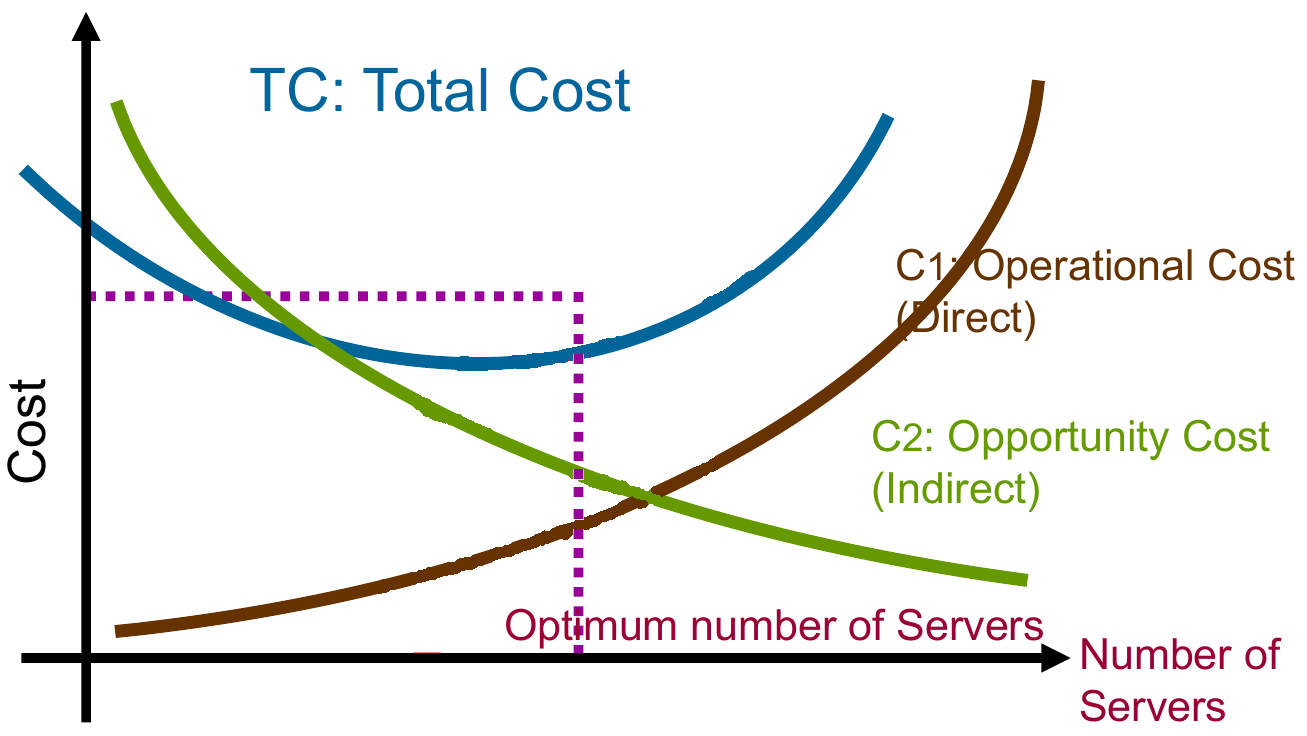
\includegraphics[
		width=14cm,
		%height=15cm
	]{Imágenes/Tema 2/Queuing motivation.png}
	\caption{
		\label{fig:unit2_qtheory}
		Queueing theory
	}
\end{figure}

\subsection{Queueing systems}

\subsubsection{Basis}

A queueing system manages traffic for a population requesting it.

Traffic is the amount of service time that has been provided to users along a period of time, so it is measured in Erlangs (E), where the unit (1 E) represents a single service being served along time, this is, the service time corresponds to time along it is being served.

A queueing system is parametrized through characteristics that are related to traffic management, such as number of users, load pattern, service characteristics and number of servers. We must then manage some performance criteria, like waiting time, blocking probability and costs.

\subsubsection{Parameters}

The parameters characterizing a queueing system are the following (some of them are redundant since they represent the same information but in another way):

\begin{itemize}
	\item Arriving rate ($u$): Amount of incoming traffic. Random variable.
	\item {
		Mean arriving rate ($\lambda$): Mean value of amount of incoming traffic:

		$ E\{u\} = \lambda $
	}
	\item {
		Time between arrivals (r): Amount of time that passes between requested services. Random variable. Its average value can be estimated from mean arriving rate:

		$ r = \frac{1}{u} \rightarrow E\{r\} = \frac{1}{\lambda} $
	}
	\item Blocking probability ($P_B$): Probability of system being stopped.
	\item {
		Effective arrival rate ($\lambda_a$): Amount of incoming traffic if we discard the traffic that can't enter the queue due to blocking phenomenom.

		$ \lambda_a = \lambda \cdot ( 1 - P_B ) $
	}
	\item {
		Queue discipline (z): It is the way in which traffic is enqueued. Most common disciplines are:

		\begin{itemize}
			\item {
				First In First Out (FIFO) / First Come First Served (FCFS): A common queue, the first element that arrived is the first element that leaves the queue.

				\begin{figure}[H]
					\centering
					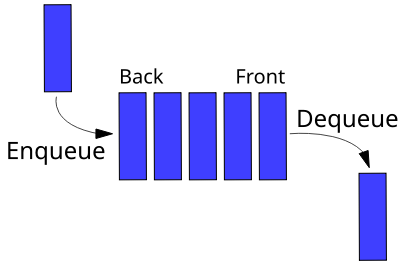
\includegraphics[
						width=7cm,
						%height=15cm
					]{Imágenes/Tema 2/Data_Queue.png}
					\caption{
						\label{fig:unit2_fifo}
						FIFO
					}
				\end{figure}
			}
			\item {
				Last in First Out (LIFO) / Last Come First Served (LCFS): A common stack, the last element that arrived is the first element that leaves the queue.

				\begin{figure}[H]
					\centering
					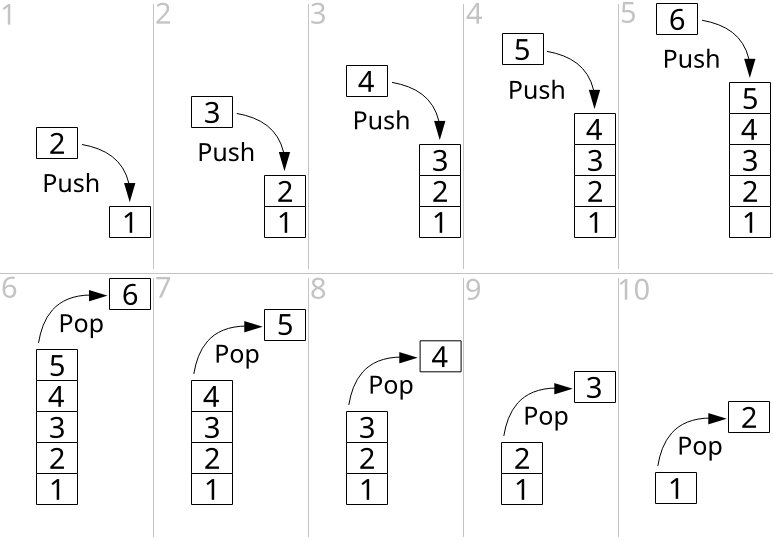
\includegraphics[
						width=8cm,
						%height=15cm
					]{Imágenes/Tema 2/Lifo_stack.png}
					\caption{
						\label{fig:unit2_lifo}
						LIFO
					}
				\end{figure}
			}
			\item Service In Random Order (SIRO): The next element leaving the system is randomly selected.
		\end{itemize}
	}
	\item Service rate ($\mu$): Rate services are completed at.
	\item {
		Service time ($s$). The amount of time a service takes to be completed. Random variable. Its average value can be estimated from service rate:

		$ E\{s\} = \frac{1}{\mu} $
	}
	\item Number of servers ($c$): Number of serving machines to attend incoming traffic.
\end{itemize}

\begin{figure}[H]
	\centering
	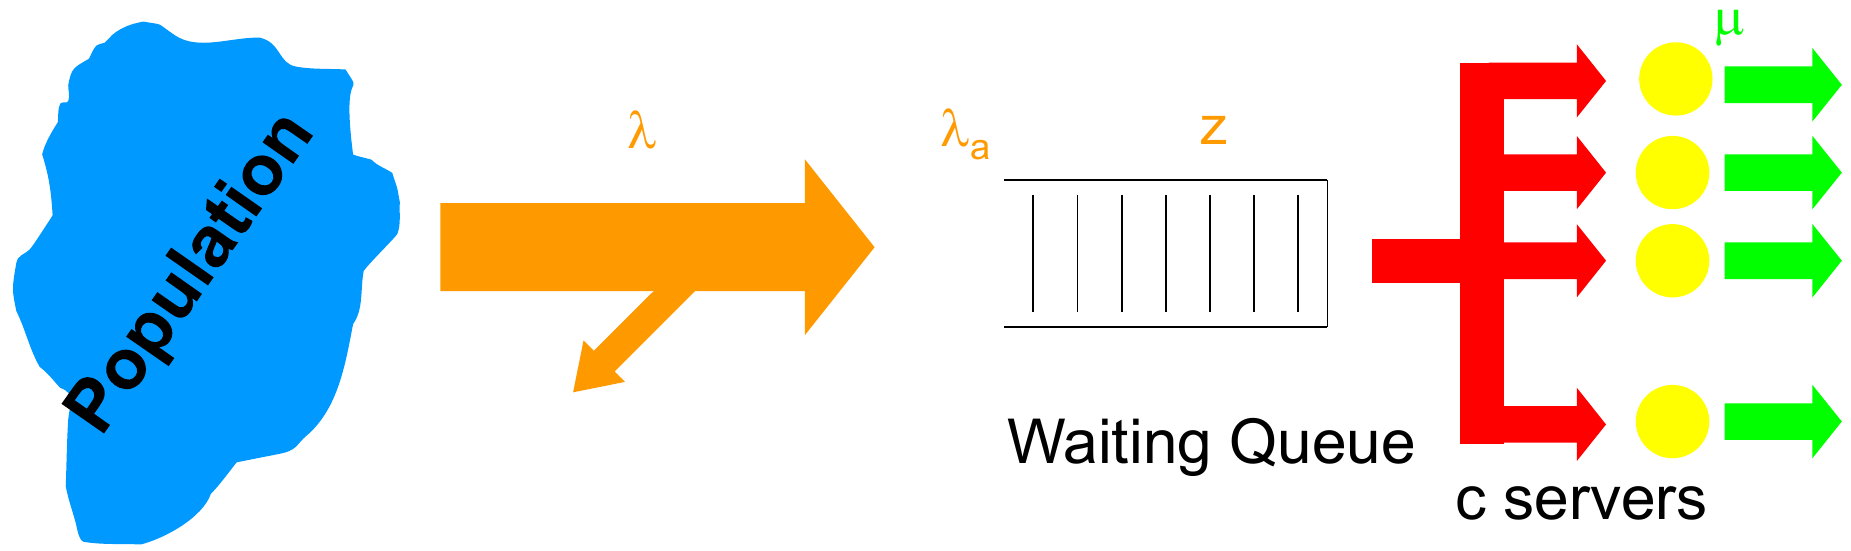
\includegraphics[
		width=12cm,
		%height=15cm
	]{Imágenes/Tema 2/Queuing system.png}
	\caption{
		\label{fig:unit2_qsystem}
		Queuing system
	}
\end{figure}

\subsubsection{Derived magnitudes}

Apart from paramaters, some aditional magnitudes derived from parameters will be useful when analyzing performance and developing solutions:

\begin{itemize}
	\item {
		Offered traffic ($A_o$): It is the amount of traffic that is said to be dispatched.

		$ A_o = \frac {E\{s\}} {E\{r\}} = \frac {\lambda} {\mu}$
	}
	\item {
		Carried traffic ($A_c$): It is the amount of traffic that is finally dispatched due to blocking phenomenom.

		$ A_c = A_o \cdot ( 1 - P_B ) = \frac {\lambda_a} {\mu} = \frac {\lambda_a} {\mu} $
	}
	\item {
		Server utilization ($\rho$):

		$ \rho = \frac {A_c} {c} = \frac {\lambda_a} {\mu \cdot c} $
	}
	\item Number of users in the servers at instant $t$ ($N_s(t)$).
	\item Number of users in the queue at instant $t$ ($N_q(t)$).
	\item {
		Number of users in the system at instant $t$ ($N(t)$):

		$ N(t) = N_s(t) + N_q(t) $
	}
	\item Number of users in the servers in continuous operation (steady state stationary regime) ($N_s$).
	\item Number of users in the queue in continuous operation (steady state stationary regime) ($N_q$).
	\item {
		Number of users in the system in continuous operation (steady state stationary regime) ($N$):

		$ N = N_s + N_q $
	}
	\item {
		Average number of users in the servers ($L_s$):

		$ L_s = E\{N_s\} $
	}
	\item {
		Average number of users in the queue ($L_q$):

		$ L_q = E\{N_q\} $
	}
	\item {
		Average number of users in the system ($L$):

		$ L = E\{N\} = L_s + L_q $
	}
	\item {
		Long-term average effective arrival rate ($\gamma$): Although this magnitude is used to demostrate Little's Law, in most of problems can be assumed to be the same as effective arrival rate $\lambda_a$.

		$ \gamma = \left. \lambda_a} \right|_{\textrm{long-term}} $
	}
	\item {
		Mean time in the servers ($W_s$):

		$ W_s = E\{s\} = \frac{1}{\mu} = \frac{L_s}{\gamma} $
	}
	\item {
		Mean time in the queue ($W_q$):

		$ W_q = \frac {L_q} {\gamma} $
	}
	\item {
		Mean time in the system ($W$):

		$ W = W_s + W_q = \frac {L} {\gamma} $
	}
\end{itemize}

\subsubsection{Little's Law}

Little's Law relates the number of users in the system with traffic. Little proved that the long-term average number of users in the servers is equal to carried traffic:

$$
	\begin{Bmatrix}
		L_s = \gamma \cdot W_s \\
		L_q = \gamma \cdot W_q
	\end{Bmatrix}
	\rightarrow
$$

$$
	\rightarrow
	L = L_s + L_q = \gamma \cdot W_s + \gamma \cdot W_q = \gamma \cdot W
	\rightarrow
$$

$$
	\rightarrow
	\left. A_c \right|_{\textrm{long-term}} = \left. \frac {\lambda_a} {\mu} \right|_{\textrm{long-term}} = \gamma \cdot W_s = L_s
$$

\subsubsection{Kendall-Lee notation}

Having a common set of defining parameters, queueing models can be refered through a common notation. We use Kendall-Lee notation:

$$
	A / B / c / K / m / z
$$

Parameters of this notation are:

\begin{itemize}
	\item {
		Arrival process ($A$): It specifies the distribution of arrival rate ($r$). Some common distributions are:
		\begin{itemize}
			\item $M$: Independent and identically distributed random variable with Poisson distribution (time between arrivals follows an exponential distribution).
			\item $D$: Independent and identically distributed random variable with determinist distribution.
			\item $GI$: Independent and identically distributed random variable with general distribution.
		\end{itemize}
	}
	\item {
		Service time distribution ($B$): It specifies the distribution of service time ($s$). Some common distributions are:
		\begin{itemize}
			\item $M$: Independent and identically distributed random variable with exponential distribution.
			\item $D$: Independent and identically distributed random variable with determinist distribution.
			\item $GI$: Independent and identically distributed random variable with general distribution.
		\end{itemize}
	}
	\item Number of servers ($c$): The number of service channels (or servers).
	\item Capacity of queue ($K$): Maximum number of customers allowed in the queue. When the number is at this maximum, further arrivals are turned away. If this number is omitted, the capacity is assumed to be infinite.
	\item Population size ($m$): The size of the population from which the customers come. If this number is omitted, the population is assumed to be unlimited, or infinite.
	\item Queue discipline ($z$): As seen in \textit{Parameters} section, it is the way in which traffic is enqueued and can be of three types, FIFO, LIFO and SIRO. When omitted, discipline is assumed to be FIFO.
\end{itemize}

\subsection{Common distributions at queueing systems}

\subsubsection{Exponential distribution}

The service time usually follows an exponential distribution, this is, we can estimate the probability that a user spends a time $t$ to be served with the density function $p_s(t)$. This also means that $p_s(t) \cdot 100\%$ of user will take a time $t$ to be served. We define the density function:

$$
	s \sim exp(\mu) \leftrightarrow P(s = t) = p_s(t) =
	\begin{Bmatrix}
		\mu \cdot e^{- \mu \cdot t}, 0 < t \\
		0, t \leq 0
	\end{Bmatrix}
	\rightarrow
	E\{s\} = \frac{1}{\mu}
$$

\begin{figure}[H]
	\centering
	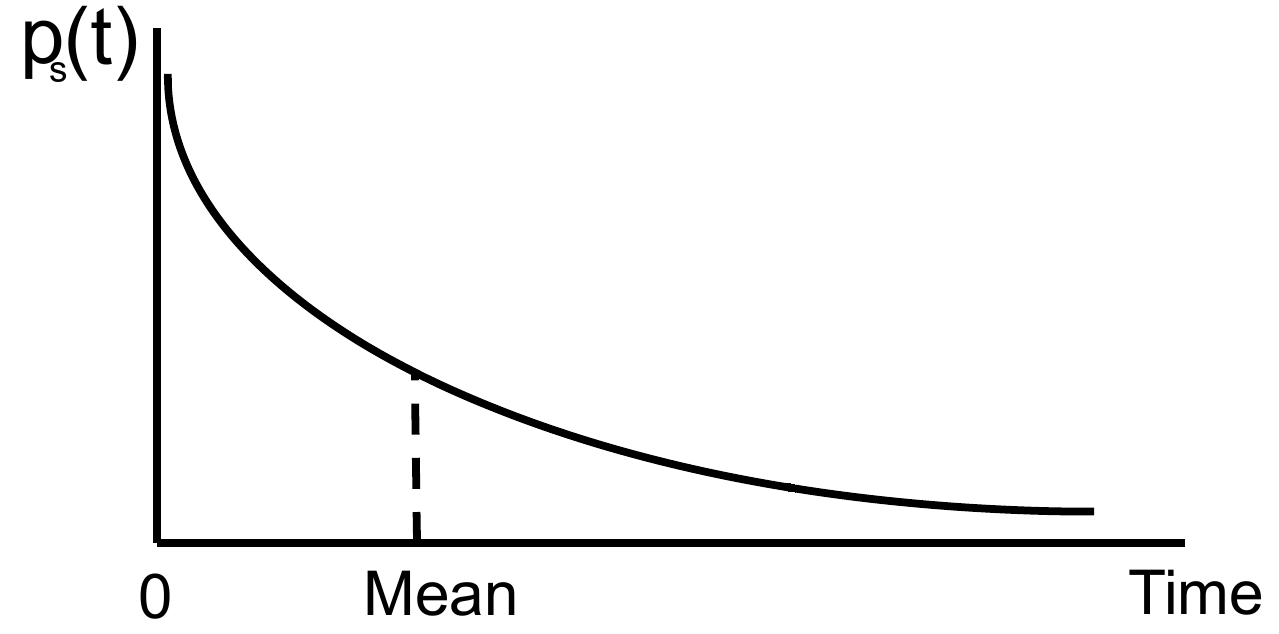
\includegraphics[
		width=10cm,
		%height=15cm
	]{Imágenes/Tema 2/Exponential distribution.png}
	\caption{
		\label{fig:unit2_exp}
		Exponential distribution
	}
\end{figure}

Distribution function can also be computed:

$$
	P(s \leq T) =
	P_s(T) =
	\int_{-\infty}^{T} p_s(t) dt =
	\int_{0}^{T} \mu \cdot e^{- \mu \cdot t} dt =
	1 - e^{- \mu \cdot t}
$$

\begin{figure}[H]
	\centering
	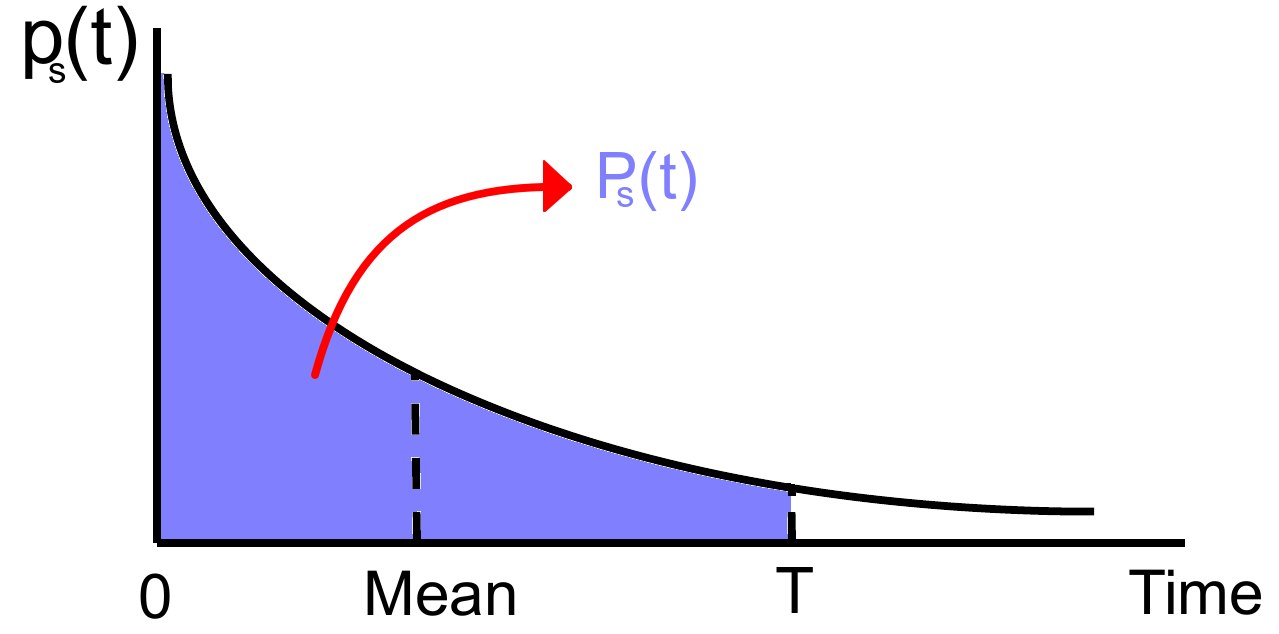
\includegraphics[
		width=10cm,
		%height=15cm
	]{Imágenes/Tema 2/Exponential distribution with area.png}
	\caption{
		\label{fig:unit2_exp_area}
		Exponential distribution area
	}
\end{figure}

\subsubsection{Poisson distribution}

Arrival rate is usually modeled by a Poisson distribution, this is, we can estimate the probability of $k$ arrivals within a unit of time with the density function. This is because we consider that time between arrivals follows an exponential distribution:

$$
	r \sim exp(\lambda) \rightarrow
	u \sim Poi(\lambda) \leftrightarrow
	P(u = k) = p_u(k) =
	\frac {\lambda^k \cdot e^{-k}} {k!} \rightarrow
	E\{u\} = \lambda
$$

\begin{figure}[H]
	\centering
	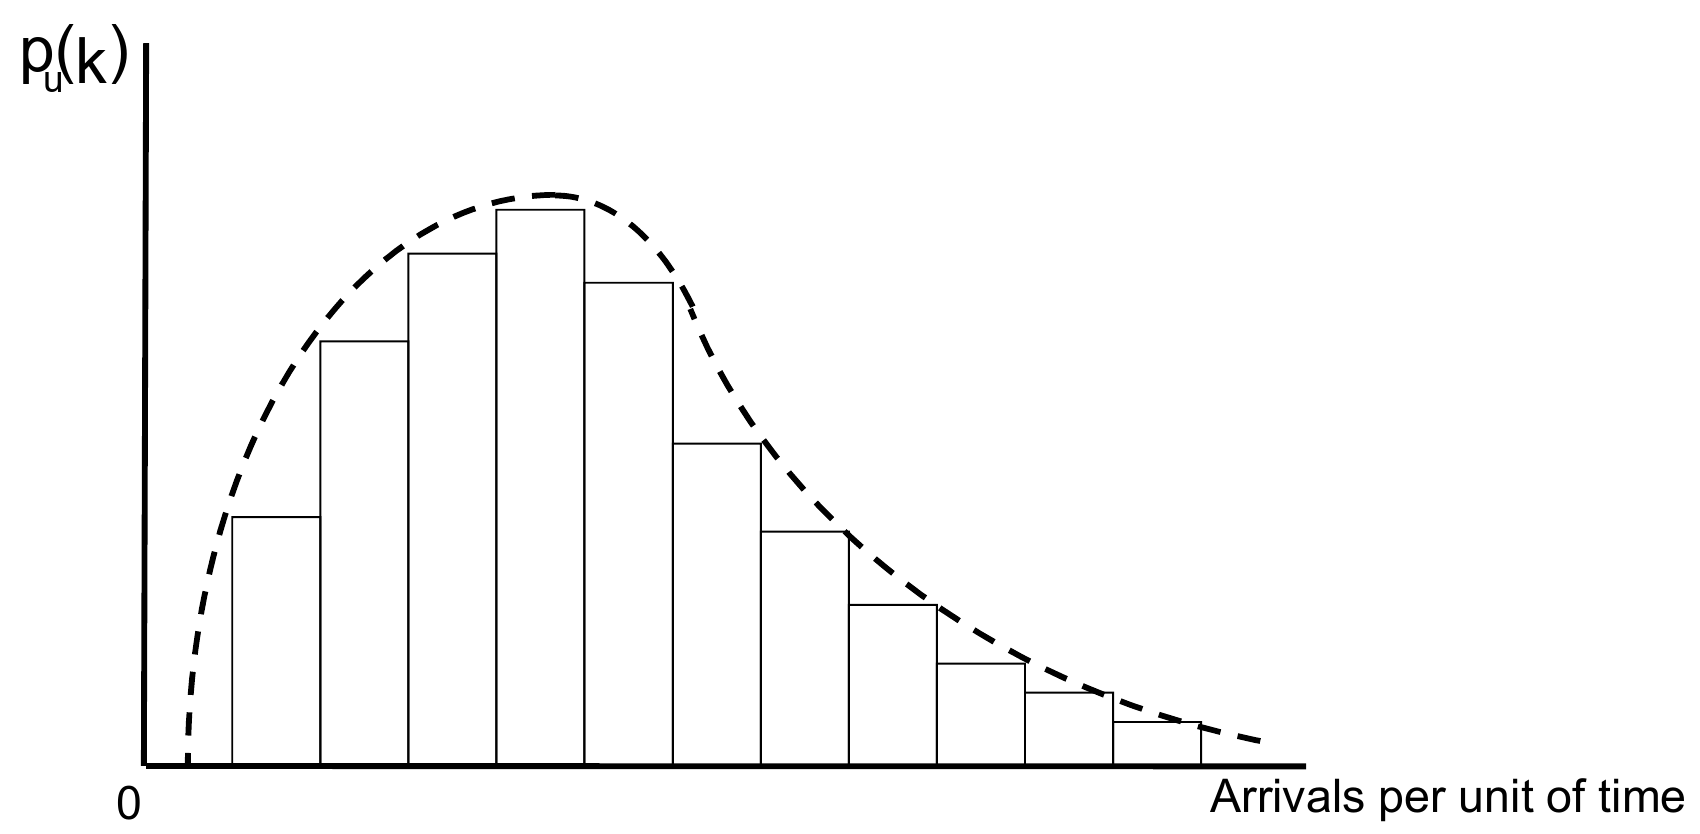
\includegraphics[
		width=10cm,
		%height=15cm
	]{Imágenes/Tema 2/Poisson distribution.png}
	\caption{
		\label{fig:unit2_poi}
		Poisson distribution
	}
\end{figure}

\subsection{Basic queueing models}

\subsubsection{$M/M/1$ model}

\paragraph{Characteristics}

The characteristics of this model are:

\begin{itemize}
	\item {
		Time between arrivals follows exponential distribution, then, arrivals rate follows Poisson distribution:

		$
			A = M \rightarrow r \sim exp(\lambda) \rightarrow u \sim Poi(\lambda)
		$
	}
	\item {
		Service time follows exponential distribution:

		$
			B = M \rightarrow s \sim exp(\mu)
		$
	}
	\item {
		One server:

		$
			c = 1
		$
	}
	\item {
		Infinite queue capacity:

		$
			K = \infty
		$
	}
	\item {
		Infinite population:

		$
			m = \infty
		$
	}
	\item {
		FIFO queue.

		$
			z = FIFO
		$
	}
	\item A certain blocking probability ($P_B$).
\end{itemize}

\begin{figure}[H]
	\centering
	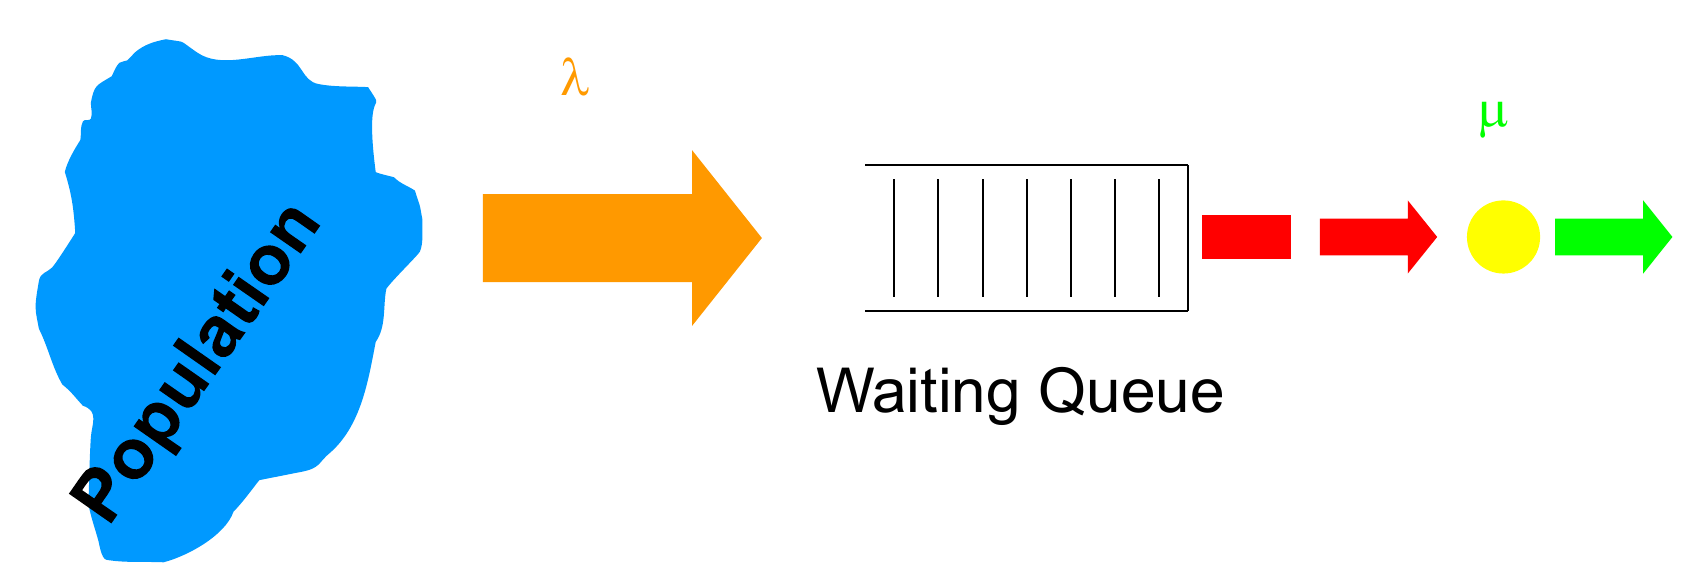
\includegraphics[
		width=12cm,
		%height=15cm
	]{Imágenes/Tema 2/M⁄M⁄1 model.png}
	\caption{
		\label{fig:unit2_MM1}
		M/M/1 model
	}
\end{figure}

\begin{figure}[H]
	\centering
	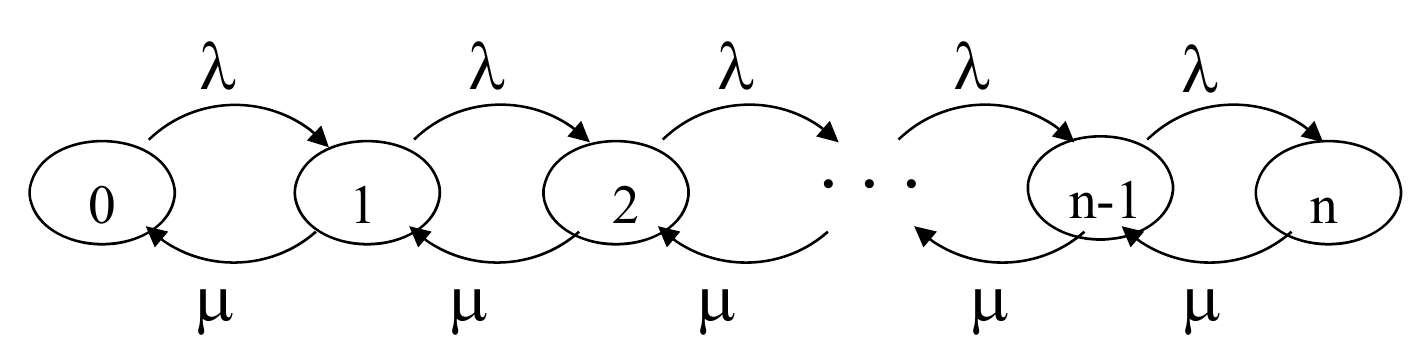
\includegraphics[
		width=12cm,
		%height=15cm
	]{Imágenes/Tema 2/MM1 model queue.png}
	\caption{
		\label{fig:unit2_MM1_queue}
		M/M/1 model queue
	}
\end{figure}

\paragraph{Properties}

The rest of properties can be derived:

\begin{itemize}
	\item {
		Server utilization (it must be less than one in order to have an stable system):

		$
			\rho =
			\frac {\lambda_a} {\mu \cdot c} \overset {\textrm{long-term}} {=}
			\frac {\gamma} {\mu \cdot c} \overset {c=1} {=}
			\frac {\gamma} {\mu} =
			\gamma \cdot W_s =
			L_s =
			\left. A_c \right|_{\textrm{long-term}} < 1
		$
	}
	\item {
		Summation $S$:

		$
			S =
			\sum_{n=0}^{\infty} \left( \frac {\lambda} {\mu} \right)^n =
			\sum_{n=0}^{\infty} A_o^n =
			\sum_{n=0}^{\infty} \left( \frac {A_c} {1 - P_B} \right)^n =
			\sum_{n=0}^{\infty} \left( \frac {c \cdot \rho} {1 - P_B} \right)^n \overset {c=1, P_B=0} {=}
			\sum_{n=0}^{\infty} \rho^n =
			\frac {1} {1 - \rho}
		$
	}
	\item {
		Probability of the server not being used:

		$
			P_0 = \frac {1} {S} = 1 - \rho
		$
	}
	\item {
		Probability of the server being used:

		$
			P(n \geq 1) = 1 - P_0 = \rho
		$
	}
	\item {
		Probability of the server being in any state:

		$
			P(n \geq 1) = \rho = \sum_{n=1}^{\infty} P_n \rightarrow P_n = (1 - \rho) \cdot \rho^n
		$
	}
	\item {
		Average number of users in the servers:

		$
			L_s = \gamma \cdot W_s = \frac {\gamma} {\mu} = \rho
		$
	}
	\item {
		Average number of users in the queue:

		$
			L_q = \sum_{i=1}^{\infty} \left[ (i-1) \cdot P_i \right] =
			\sum_{i=1}^{\infty} \left[ (i-1) \cdot (1-\rho) \cdot \rho^i \right] =
			\frac {\rho^2} {1-\rho}
		$
	}
	\item {
		Average number of users in the system:

		$
			L = \sum_{i=1}^{\infty} \left[ i \cdot P_i \right] =
			\sum_{i=1}^{\infty} \left[ i \cdot (1-\rho) \cdot \rho^i \right] =
			\frac {\rho} {1-\rho}
		$
	}
	\item {
		Mean time in servers:

		$
			W_s = \frac {1} {\mu}
		$
	}
	\item {
		Mean time in the queue:

		$
			W_q = \frac {L_q} {\gamma} = \frac {\frac{\rho^2}{1-\rho}} {\frac{\rho}{W_s}} =
			W_s \cdot \frac {\rho} {1-\rho} =
			\frac {\rho} {\mu \cdot (1-\rho)} \overset {\rho=1} {=} \infty
		$
	}
	\item {
		Mean time in the system:

		$
			W =
			W_s + W_q =
			W_s + W_s \cdot \frac {\rho} {1-\rho} =
			\frac {W_s} {1-\rho} =
			\frac {1} {\mu \cdot (1-\rho)} \overset {\rho=1} {=} \infty
		$
	}
\end{itemize}

\subsubsection{$M/M/c$ model}

\paragraph{Characteristics}

The characteristics of this model are:

\begin{itemize}
	\item {
		Time between arrivals follows exponential distribution, then, arrivals rate follows Poisson distribution:

		$
			A = M \rightarrow r \sim exp(\lambda) \rightarrow u \sim Poi(\lambda)
		$
	}
	\item {
		Service time follows exponential distribution:

		$
			B = M \rightarrow s \sim exp(\mu)
		$
	}
	\item {
		$c$ servers:

		$
			c = c
		$
	}
	\item {
		Infinite queue capacity:

		$
			K = \infty
		$
	}
	\item {
		Infinite population:

		$
			m = \infty
		$
	}
	\item {
		FIFO queue.

		$
			z = FIFO
		$
	}
	\item A certain blocking probability ($P_B$).
\end{itemize}

\begin{figure}[H]
	\centering
	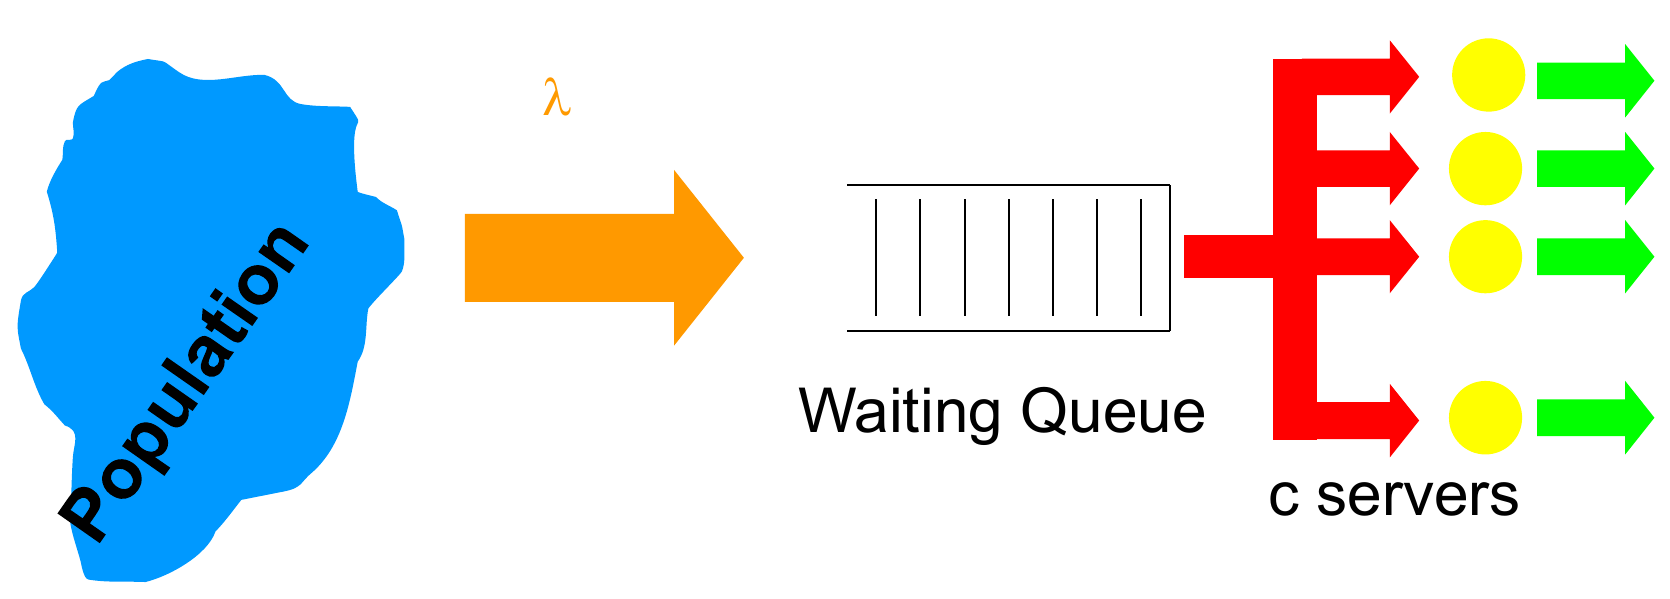
\includegraphics[
		width=12cm,
		%height=15cm
	]{Imágenes/Tema 2/M⁄M⁄c model.png}
	\caption{
		\label{fig:unit2_MMc}
		M/M/c model
	}
\end{figure}

\begin{figure}[H]
	\centering
	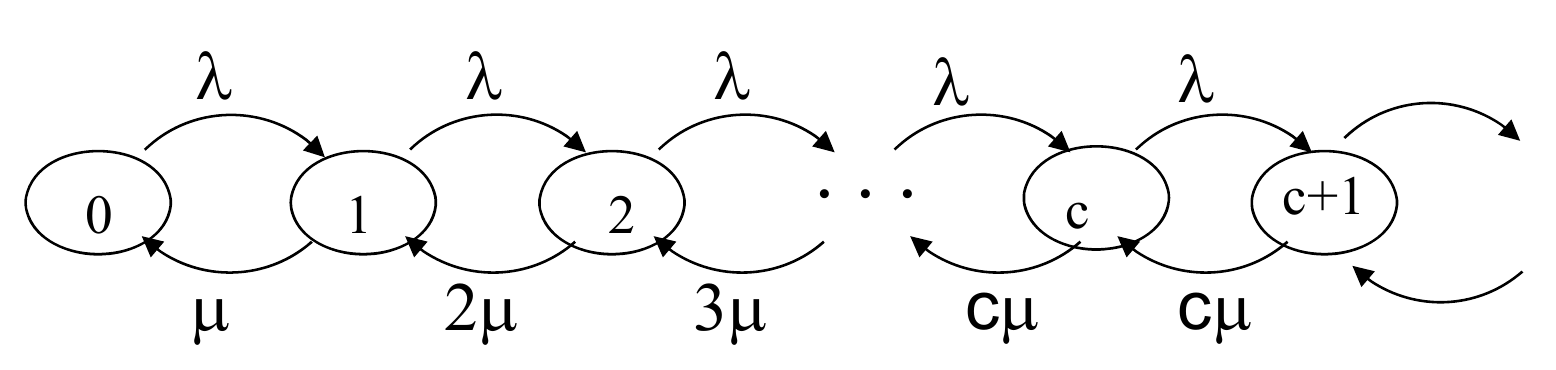
\includegraphics[
		width=12cm,
		%height=15cm
	]{Imágenes/Tema 2/MMc model queue.png}
	\caption{
		\label{fig:unit2_MMc_queue}
		M/M/c model queue
	}
\end{figure}

\paragraph{Erlang C}

As can be infered, estimating waiting time distribution in this model is more complex. The probability of a customer having to wait on the queue due to having all servers occupied can be computed iteratively with Erlang C function, which depends on the incoming offered traffic $A_o$ and the number of servers $c$:

$$
	C(A_o, c) = \frac {A_{o}^c} {c! \cdot (1-\rho)} P_0 =  \frac {A_{o}^c} { c! \cdot (1-\rho) \cdot \left( \sum_{n=0}^{c-1} \left( \frac {A_{o}^n} {n!} \right) + \frac {A_{o}^c} {c! \cdot (1-\rho)} \right) }
$$

\begin{figure}[H]
	\centering
	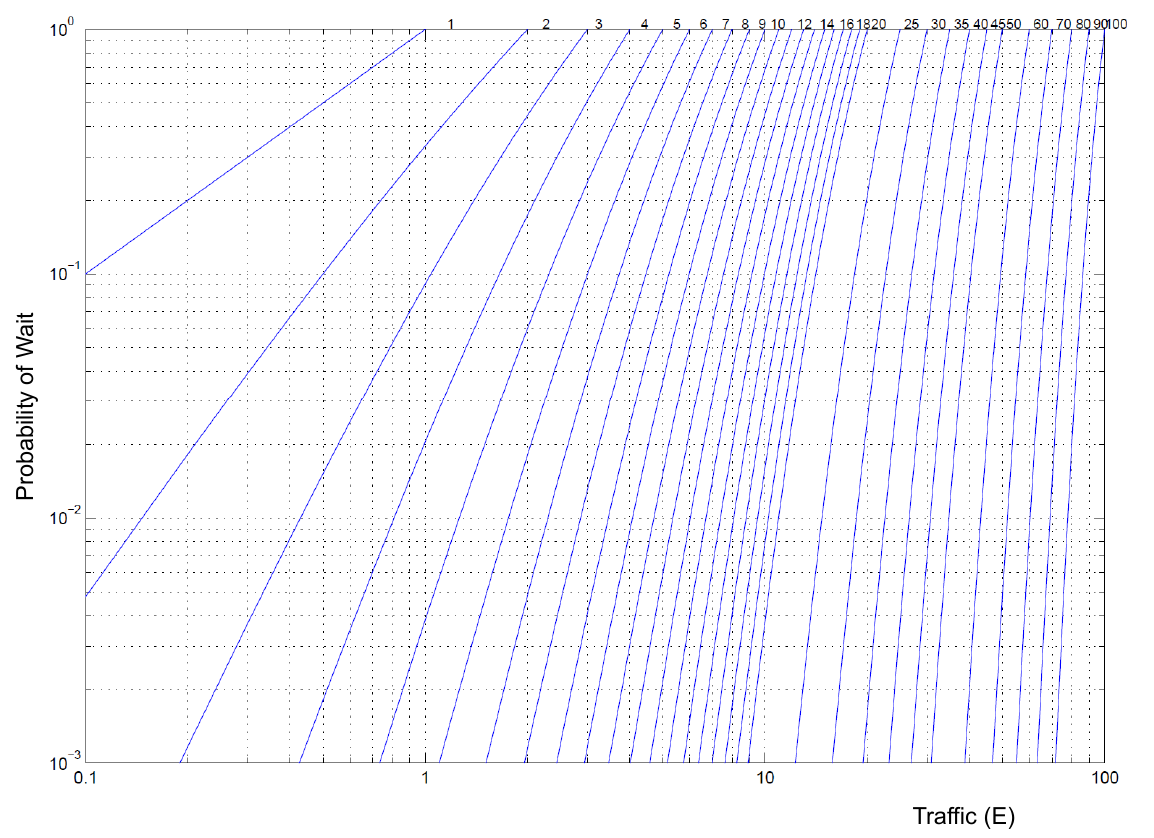
\includegraphics[
		width=14cm,
		%height=15cm
	]{Imágenes/Tema 2/Erlang C.png}
	\caption{
		\label{fig:unit2_erlangC}
		Erlang C for M/M/c model
	}
\end{figure}

\paragraph{Properties}

The rest of properties can be derived:

\begin{itemize}
	\item {
		Server utilization (it must be less than one in order to have an stable system):

		$
			\rho =
			\frac {\lambda_a} {\mu \cdot c} \overset {\textrm{long-term}} {=}
			\frac {\gamma} {\mu \cdot c} =
			\frac {\gamma \cdot W_s} {c} =
			\frac {L_s} {c} =
			\frac {\left. A_c \right|_{\textrm{long-term}}} {c}
			< 1
		$
	}
	\item {
		Summation $S$:

		$
			S =
			\sum_{n=0}^{c-1} \left( \frac {A_{o}^n} {n!} \right) + \frac {A_{o}^c} {c! \cdot (1-\rho)}
		$
	}
	\item {
		Probability of the server not being used:

		$
			P_0 = \frac {1} {S} = \frac {1} {\sum_{n=0}^{c-1} \left( \frac {A_{o}^n} {n!} \right) + \frac {A_{o}^c} {c! \cdot (1-\rho)}}
		$
	}
	\item {
		Probability of the server being used:

		$
			P(n \geq 1) = 1 - P_0 = 1 - \frac {1} {S}
		$
	}
	\item {
		Probability of the server being in any state:

		$
			P(n \geq 1) = 1 - \frac {1} {S} = \sum_{n=1}^{\infty} P_n \rightarrow
			P_n = \frac {1} {S} \cdot \left( 1 - \frac {1} {S} \right)^n
		$
	}
	\item {
		Probability of having to wait in the queue:

		$
			P_{wait} = C(A_o, c) = \frac {A_{o}^c} {c! \cdot (1-\rho)} P_0 =  \frac {A_{o}^c} { c! \cdot (1-\rho) \cdot \left( \sum_{n=0}^{c-1} \left( \frac {A_{o}^n} {n!} \right) + \frac {A_{o}^c} {c! \cdot (1-\rho)} \right) }
		$
	}
	\item {
		Average number of users in the servers:

		$
			L_s = \gamma \cdot W_s = \frac {\gamma} {\mu} = c \cdot \rho
		$
	}
	\item {
		Average number of users in the queue:

		$
			L_q = \frac {\rho} {1-\rho} \cdot C(A_o, c)
		$
	}
	\item {
		Average number of users in the system:

		$
			L = c \cdot \rho + \frac {\rho} {1-\rho} \cdot C(A_o, c)
		$
	}
	\item {
		Mean time in servers:

		$
			W_s = \frac {1} {\mu}
		$
	}
	\item {
		Mean time in the queue:

		$
			W_q =
			\frac {W_s} {c \cdot (1-\rho)} \cdot C(A_o, c) =
			\frac {1} {\mu \cdot c \cdot (1-\rho)} \cdot C(A_o, c)
		$
	}
	\item {
		Mean time in the system:

		$
			W =
			W_s + W_q =
			W_s + \frac {W_s} {c \cdot (1-\rho)} \cdot C(A_o, c) =
			\frac {1} {\mu} + \frac {1} {\mu \cdot c \cdot (1-\rho)} \cdot C(A_o, c)
			\overset {\rho=1} {=} \infty
		$
	}
	\item {
		Distribution of mean time in the queue:

		$
			P(W_q < t) = 1 - C(A_o, c) \cdot e^{- c \cdot \mu \cdot (1-\rho) \cdot t}
		$
	}
\end{itemize}

\subsubsection{$M/M/c/c$ model}

\paragraph{Characteristics}

The characteristics of this model are:

\begin{itemize}
	\item {
		Time between arrivals follows exponential distribution, then, arrivals rate follows Poisson distribution:

		$
			A = M \rightarrow r \sim exp(\lambda) \rightarrow u \sim Poi(\lambda)
		$
	}
	\item {
		Service time follows exponential distribution:

		$
			B = M \rightarrow s \sim exp(\mu)
		$
	}
	\item {
		$c$ servers:

		$
			c = c
		$
	}
	\item {
		Queue capacity is limited to number of servers:

		$
			K = c
		$
	}
	\item {
		Infinite population:

		$
			m = \infty
		$
	}
	\item {
		FIFO queue.

		$
			z = FIFO
		$
	}
	\item A certain blocking probability ($P_B$).
\end{itemize}

\begin{figure}[H]
	\centering
	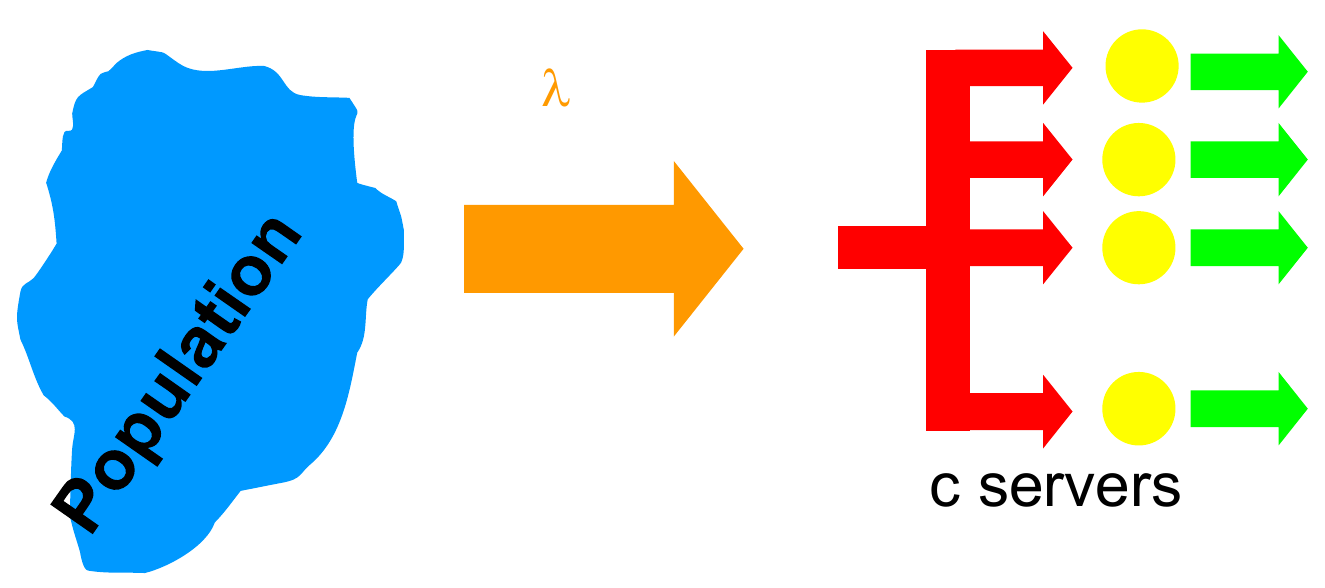
\includegraphics[
		width=12cm,
		%height=15cm
	]{Imágenes/Tema 2/M⁄M⁄c⁄c model.png}
	\caption{
		\label{fig:unit2_MMcc}
		M/M/c/c model
	}
\end{figure}

\begin{figure}[H]
	\centering
	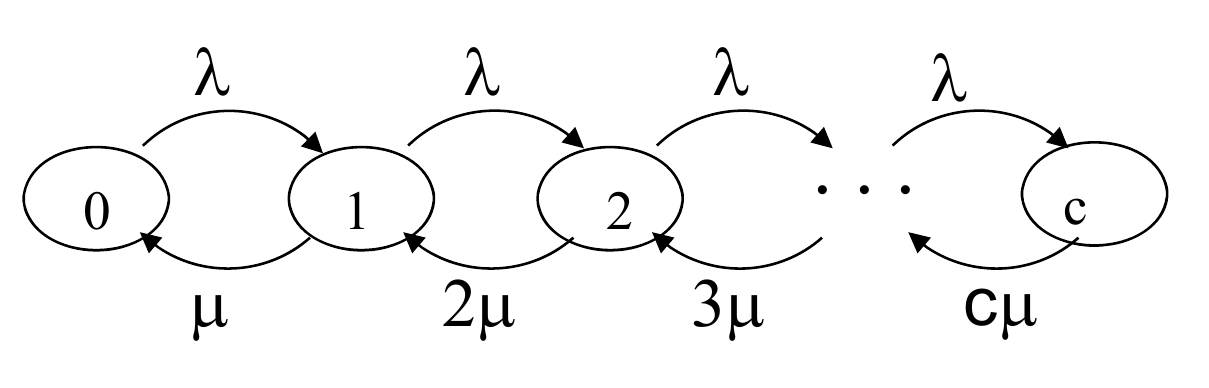
\includegraphics[
		width=12cm,
		%height=15cm
	]{Imágenes/Tema 2/MMcc model queue.png}
	\caption{
		\label{fig:unit2_MMcc_queue}
		M/M/c/c model queue
	}
\end{figure}

\paragraph{Erlang B}

The fact that the queue has the same size as the number of servers equals to not having queue but a fixed number of $c$ servers. As can be infered, apart from external blocking sources, this system itself will cause blocking when there are more calls than available servers. Blocking probability can be computed iteratively with Erlang B function, which depends on the incoming offered traffic $A_o$ and the number of servers $c$:

$$
	B(A_o, c) = P_0 \cdot \frac {A_{o}^c} {c!}= \frac {A_{o}^c} { c! \cdot \left( \sum_{n=0}^{c} \left( \frac {A_{o}^n} {n!} \right) \right) }
$$

\begin{figure}[H]
	\centering
	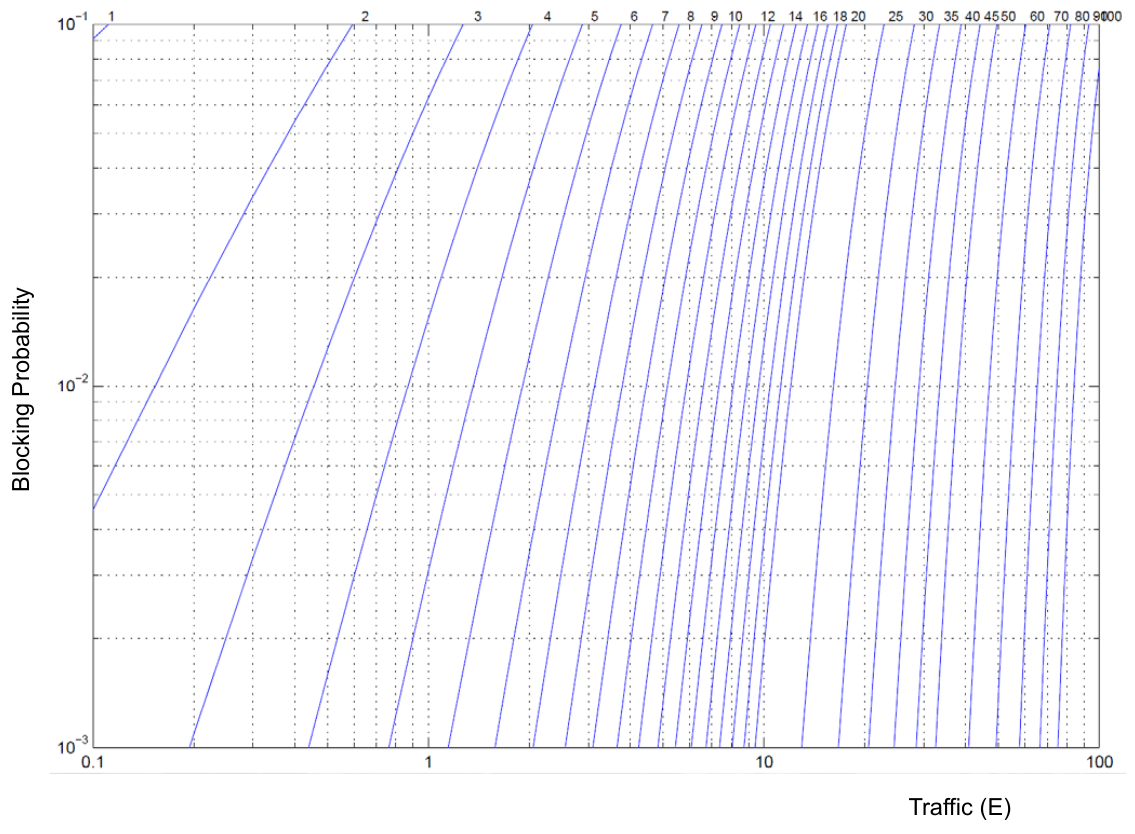
\includegraphics[
		width=14cm,
		%height=15cm
	]{Imágenes/Tema 2/Erlang B.png}
	\caption{
		\label{fig:unit2_erlangB}
		Erlang B for M/M/c/c model
	}
\end{figure}

\paragraph{Properties}

The rest of properties can be derived:

\begin{itemize}
	\item {
		Server utilization (it must be less than one in order to have an stable system):

		$
			\rho =
			\frac {\lambda_a} {\mu \cdot c} \overset {\textrm{long-term}} {=}
			\frac {\gamma} {\mu \cdot c} =
			\frac {\gamma \cdot W_s} {c} =
			\frac {L_s} {c} =
			\frac {\left. A_c \right|_{\textrm{long-term}}} {c}
			< 1
		$
	}
	\item {
		Summation $S$:

		$
			S = \sum_{n=0}^{c} \left( \frac {A_{o}^n} {n!} \right)
		$
	}
	\item {
		Probability of the server not being used:

		$
			P_0 = \frac {1} {S} = \frac {1} {\sum_{n=0}^{c} \left( \frac {A_{o}^n} {n!} \right)}
		$
	}
	\item {
		Probability of the server being used:

		$
			P(n \geq 1) = 1 - P_0 = 1 - \frac {1} {S}
		$
	}
	\item {
		Probability of the server being in any state:

		$
			P(n \geq 1) = 1 - \frac {1} {S} = \sum_{n=1}^{\infty} P_n \rightarrow
			P_n = \frac {1} {S} \cdot \left( 1 - \frac {1} {S} \right)^n =
			P_0 \cdot \frac {A_{o}^n} {c!} = \frac {\frac{A_{o}^n}{c!}} {\sum_{k=0}^c \left( \frac {A_{o}^k} {k!} \right)}
		$
	}
	\item {
		Probability of the server being in any state:

		$
			P(n \geq 1) = 1 - \frac {1} {S} = \sum_{n=1}^{\infty} P_n \rightarrow
			P_n = \frac {1} {S} \cdot \left( 1 - \frac {1} {S} \right)^n
		$
	}
	\item {
		Probability of having to wait in the queue:

		$
			P_{wait} = 0
		$
	}
	\item {
		Blocking probability:

		$
			P_{\textrm{blocking}} = B(A_o, c) = P_0 \cdot \frac {A_{o}^c} {c!} = \frac {\frac{A_{o}^c}{c!}} {\sum_{n=0}^c \left( \frac {A_{o}^n} {n!} \right)} = \frac {A_{o}^c} { c! \cdot \left( \sum_{n=0}^{c} \left( \frac {A_{o}^n} {n!} \right) \right) }
		$
	}
	\item {
		Carried traffic:

		$
			A_c = A_o \cdot \left( 1 - B(A_o, c) \right)
		$
	}
	\item {
		Average number of users in the servers:

		$
			L_s = \gamma \cdot W_s = \frac {\gamma} {\mu} = c \cdot \rho
		$
	}
	\item {
		Average number of users in the queue:

		$
			L_q = 0
		$
	}
	\item {
		Average number of users in the system:

		$
			L = L_s = c \cdot \rho
		$
	}
	\item {
		Mean time in servers:

		$
			W_s = \frac {1} {\mu}
		$
	}
	\item {
		Mean time in the queue:

		$
			W_q = 0
		$
	}
	\item {
		Mean time in the system:

		$
			W =
			W_s + W_q =
			W_s =
			\frac {1} {\mu}
		$
	}
\end{itemize}

\subsubsection{Summary}

\begin{tabular}{|c|c|c|c|}
	\hline
	& $M/M/1$ & $M/M/c$ & $M/M/c/c$ \\
	\hline
	$A$ & \multicolumn{3}{c|}{$M$} \\
	\hline
	$B$ & \multicolumn{3}{c|}{$M$} \\
	\hline
	$c$ & $1$ & \multicolumn{2}{c|}{$c$} \\
	\hline
	$K$ & \multicolumn{2}{c|}{$\infty$} & $c$ \\
	\hline
	$m$ & \multicolumn{3}{c|}{$\infty$} \\
	\hline
	$z$ & \multicolumn{3}{c|}{$FIFO$} \\
	\hline
	$r$ & \multicolumn{3}{c|}{$\sim exp(\lambda)$} \\
	\hline
	$u$ & \multicolumn{3}{c|}{$\sim Poi(\lambda)$} \\
	\hline
	$s$ & \multicolumn{3}{c|}{$\sim exp(\mu)$} \\
	\hline
\end{tabular}

\begin{landscape}

\begin{tabular}{|c|c|c|c|}
	\hline
	& $M/M/1$ & $M/M/c$ & $M/M/c/c$ \\
	\hline
	$\rho$ & $\frac {\lambda_a} {\mu} = A_c = L_s < 1$ & \multicolumn{2}{c|}{$\frac {\lambda_a} {\mu \cdot c} = \frac {A_c} {c} = \frac {L_s} {c} < 1$} \\
	\hline
	$S$ & $\frac {1} {1 - \rho}$ & $\sum_{n=0}^{c-1} \left( \frac {A_{o}^n} {n!} \right) + \frac {A_{o}^c} {c! \cdot (1-\rho)}$ & $\sum_{n=0}^{c} \left( \frac {A_{o}^n} {n!} \right)$ \\
	\hline
	$P_0$ & $\frac {1} {S} = 1 - \rho$ & $\frac {1} {S} = \frac {1} {\sum_{n=0}^{c-1} \left( \frac {A_{o}^n} {n!} \right) + \frac {A_{o}^c} {c! \cdot (1-\rho)}}$ & $\frac {1} {S} = \frac {1} {\sum_{n=0}^{c} \left( \frac {A_{o}^n} {n!} \right)}$ \\
	\hline
	$P(n \geq 1)$ & $1 - P_0 = \rho$ & $1 - P_0$ & $1 - P_0$ \\
	\hline
	$P_n$ & $(1 - \rho) \cdot \rho^n$ & $\frac {1} {S} \cdot \left( 1 - \frac {1} {S} \right)^n$ & $\frac {\frac{A_{o}^n}{c!}} {\sum_{k=0}^c \left( \frac {A_{o}^k} {k!} \right)}$ \\
	\hline
	$L_s$ & $A_c = \frac {\lambda_a} {\mu} = \rho$ & \multicolumn{2}{c|}{$A_c = \frac {\lambda_a} {\mu} = c \cdot \rho$} \\
	\hline
	$L_q$ & $\frac {\rho^2} {1-\rho}$ & $\frac {\rho} {1-\rho} \cdot C(A_o, c)$ & $0$ \\
	\hline
	$L$ & $\frac {\rho} {1-\rho}$ & $c \cdot \rho + \frac {\rho} {1-\rho} \cdot C(A_o, c)$ & $L_s = A_c = \frac {\lambda_a} {\mu} = c \cdot \rho$ \\
	\hline
	$W_s$ & \multicolumn{3}{c|}{$\frac {1} {\mu}$} \\
	\hline
	$W_q$ & $W_s \cdot \frac {\rho} {1-\rho} = \frac {\rho} {\mu \cdot (1-\rho)}$ & $\frac {W_s} {c \cdot (1-\rho)} \cdot C(A_o, c) = \frac {1} {\mu \cdot c \cdot (1-\rho)} \cdot C(A_o, c)$ & $0$ \\
	\hline
	$W$ & $\frac {W_s} {1-\rho} = \frac {1} {\mu \cdot (1-\rho)}$ & $W_s + \frac {W_s} {c \cdot (1-\rho)} \cdot C(A_o, c) = \frac {1} {\mu} + \frac {1} {c \cdot \mu \cdot (1-\rho)} \cdot C(A_o, c)$ & $W_s = \frac {1} {\mu}$ \\
	\hline
	$P_{wait}$ & $A_o = \frac {\lambda} {\mu}$ & $C(A_o, c)$ & $0$ \\
	\hline
	$P_{blocking}$ & \multicolumn{2}{c|}{$0$} & $B(A_o, c)$ \\
	\hline
	$P(W_q < t)$ & $1 - A_o \cdot e^{- \mu \cdot (1-A_o) \cdot t}$ & $1 - C(A_o, c) \cdot e^{- c \cdot \mu \cdot (1-\rho) \cdot t}$ & \\
	\hline
	$P(W_q > t)$ & $A_o \cdot e^{- \mu \cdot (1-A_o) \cdot t}$ & $C(A_o, c) \cdot e^{- c \cdot \mu \cdot (1-\rho) \cdot t}$ & \\
	\hline
\end{tabular}

\end{landscape}

\section{Telephony network architecture}

\subsection{Hierarchical networks}

\subsubsection{Introduction}

The main reason for the usage of hierarchical networks is the reduction of the number of connections among subscribers:

\begin{itemize}
	\item If we have $N$ telephones, we need $C = \frac {N \cdot (N - 1)} {2}$ connections for interconnecting each other.
	\item If we include a local exchange for a certain area, the number of connections is reduced to $C = N$.
\end{itemize}
Each of these connections is denoted "subscriber loop" or "subscriber line". The exchange that only connects subscribers from the same area is denoted "local exchange" or "toll center".

\subsubsection{Hierarchy}

If toll centers were not interconnected, only local calls could be carried out. Since we need to interconnect the toll centers with each other and they are too much (thousand in Spain), a new exchange is needed, denoted as primary center. Some primary centers has also their own subscribers. The link between toll and primary centers is denoted as primary section or trunk. The primary area is defined by the primary center and everything under it (local centers and subscribers).

Again, the number of primary centers is too high and thus, a higher level exchange is defined, denoted as sectional center or secondary center. Each primary center depends on one and only one sectional center. However, the same sectional center can handle several primary centers. No subscribers are allowed in sectional centers. The link between primary and secondary is denoted as secondary path. The secondary area is defined by everything under the sectional center (usually a province).

Following with the hierarchy, we have the regional center or tertiary centers (in Spain, there are regional centers that are interconnected in mesh with each other). These exchanges usually are located in a region. Each sectional center depends on one and only one tertiary center. However, a regional center can handle several secondary centers. The tertiary path is the link between a sectional and a tertiary center. Again, the tertiary area is defined by everything under a regional center.

Following the hierarchy, we find quaternary and international gateway.

The hierarchy is defined as a set of subscribers and exchanges interconnected, where each one depends only on the higher layer hierarchy center. The hierarchy paths are denoted as subscriber loop, primary section, secondary section, \ldots All these paths are the final trunk (end sections). A Final Trunk Group (FTG) is the set of final trunks that interconnect two subscribers by using only the hierarchy network.

\begin{figure}[H]
	\centering
	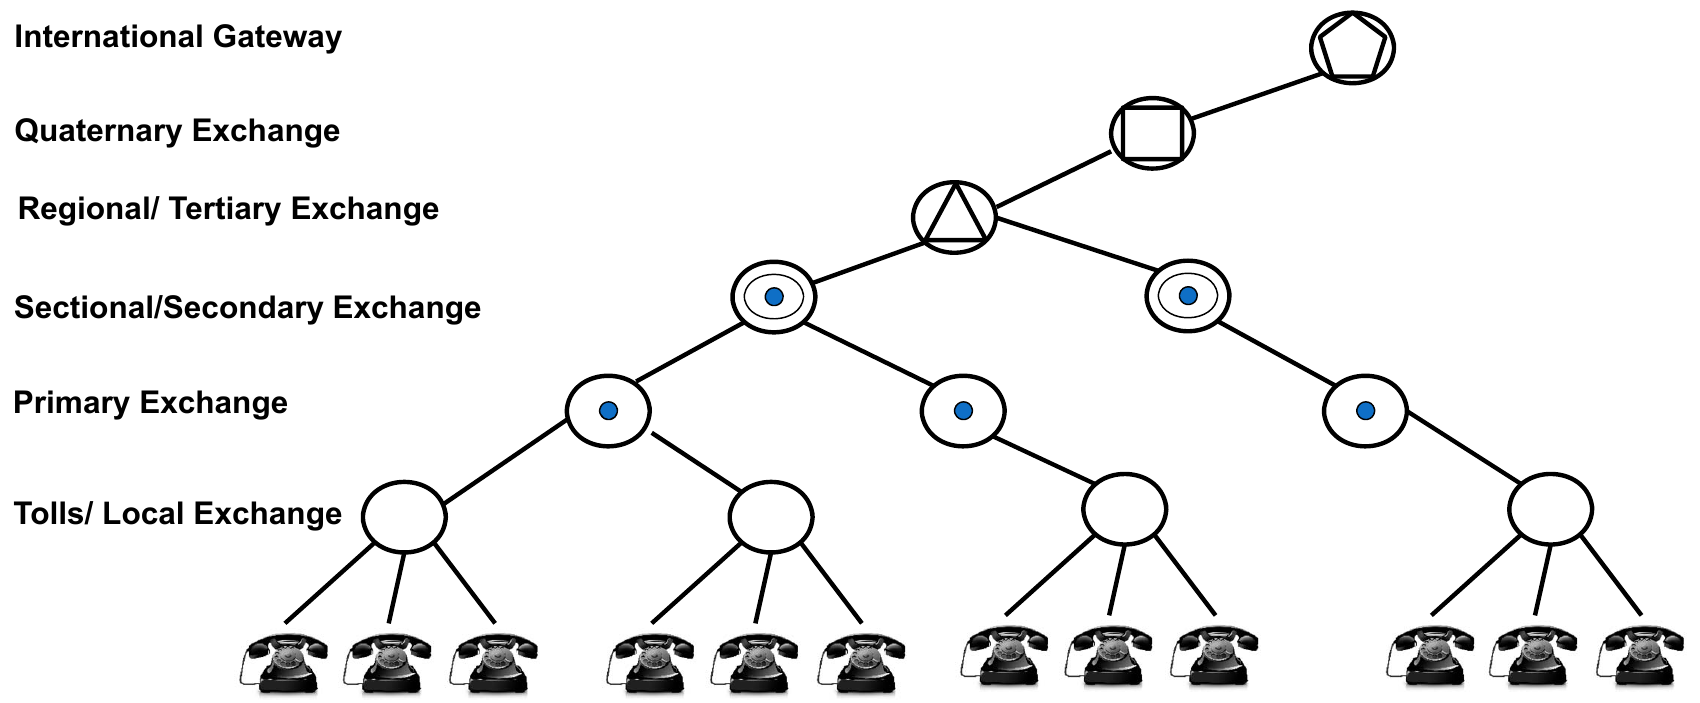
\includegraphics[
		width=14cm,
		%height=15cm
	]{Imágenes/Tema 2/Hierarchical network.png}
	\caption{
		\label{fig:unit2_hierarchy}
		Hierarchical network
	}
\end{figure}

The length of the end path depends on the distance between subscribers in the hierarchical network. For example, as shown in figure \ref{fig:unit2_dist_example}. Some paths would be:

\begin{itemize}
	\item $A \rightarrow B: A, CL1, B$
	\item $A \rightarrow C: A, CL1, CP1, CS2, CP2, CL2, C$
	\item $A \rightarrow D: A, CL1, CP1, CS2, CP2, CL3, D$
	\item $A \rightarrow E: A, CL1, CP1, CS2, CP2, CL3, E$
\end{itemize}

\begin{figure}[H]
	\centering
	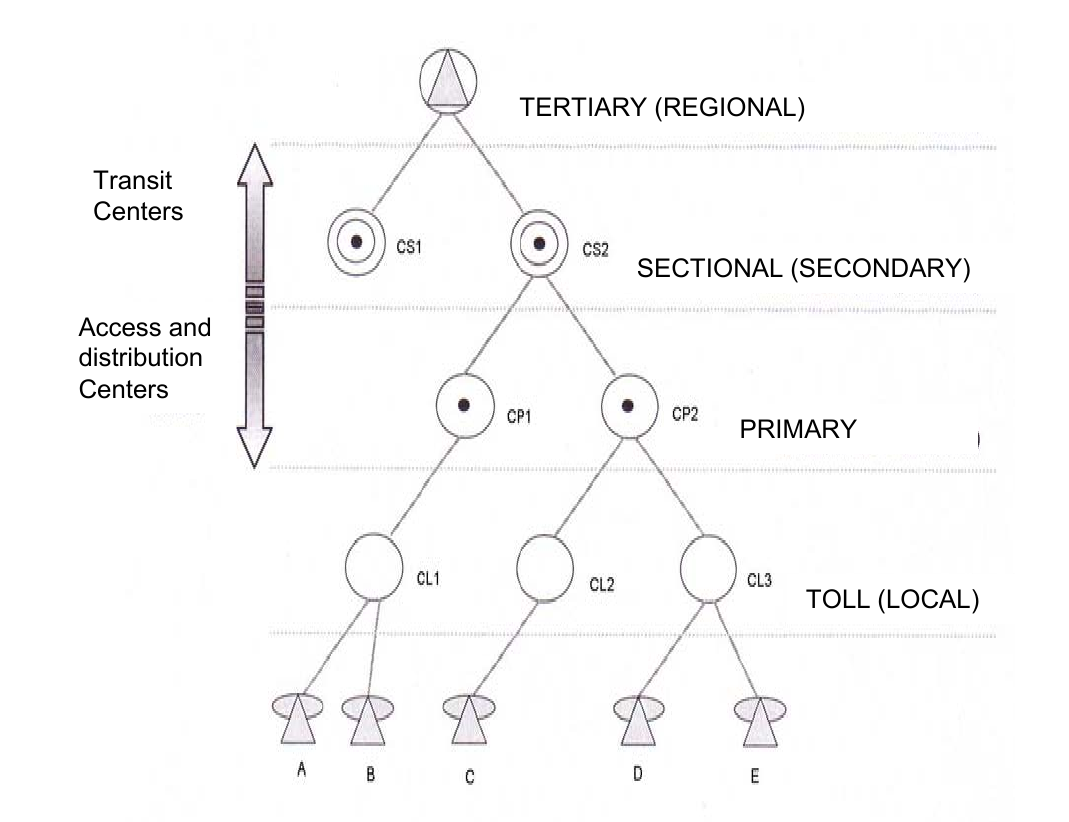
\includegraphics[
		width=12cm,
		%height=15cm
	]{Imágenes/Tema 2/Path distance example.png}
	\caption{
		\label{fig:unit2_dist_example}
		Path distance example
	}
\end{figure}

\subsubsection{High usage trunks}

The high usage trunks (HU) are superimposed to the hierarchical network. High usage trunks are
the direct sections and tandem centers. A direct section or high usage trunk is a set of links
interconnecting two exchanges that do not depend hierarchically. High usage trunks are selected
first for routing, and only when they are congested the traffic use final sections.

The following High Usage Trunks are allowed:

\begin{itemize}
	\item From toll to toll.
	\item From primary to primary.
	\item From sectional to sectional.
	\item From toll to primary that do not depend hierarchically.
	\item From primary to sectional that do not depend hierarchically.
	\item From sectional to regional that do not depend hierarchically.
\end{itemize}

\begin{figure}[H]
	\centering
	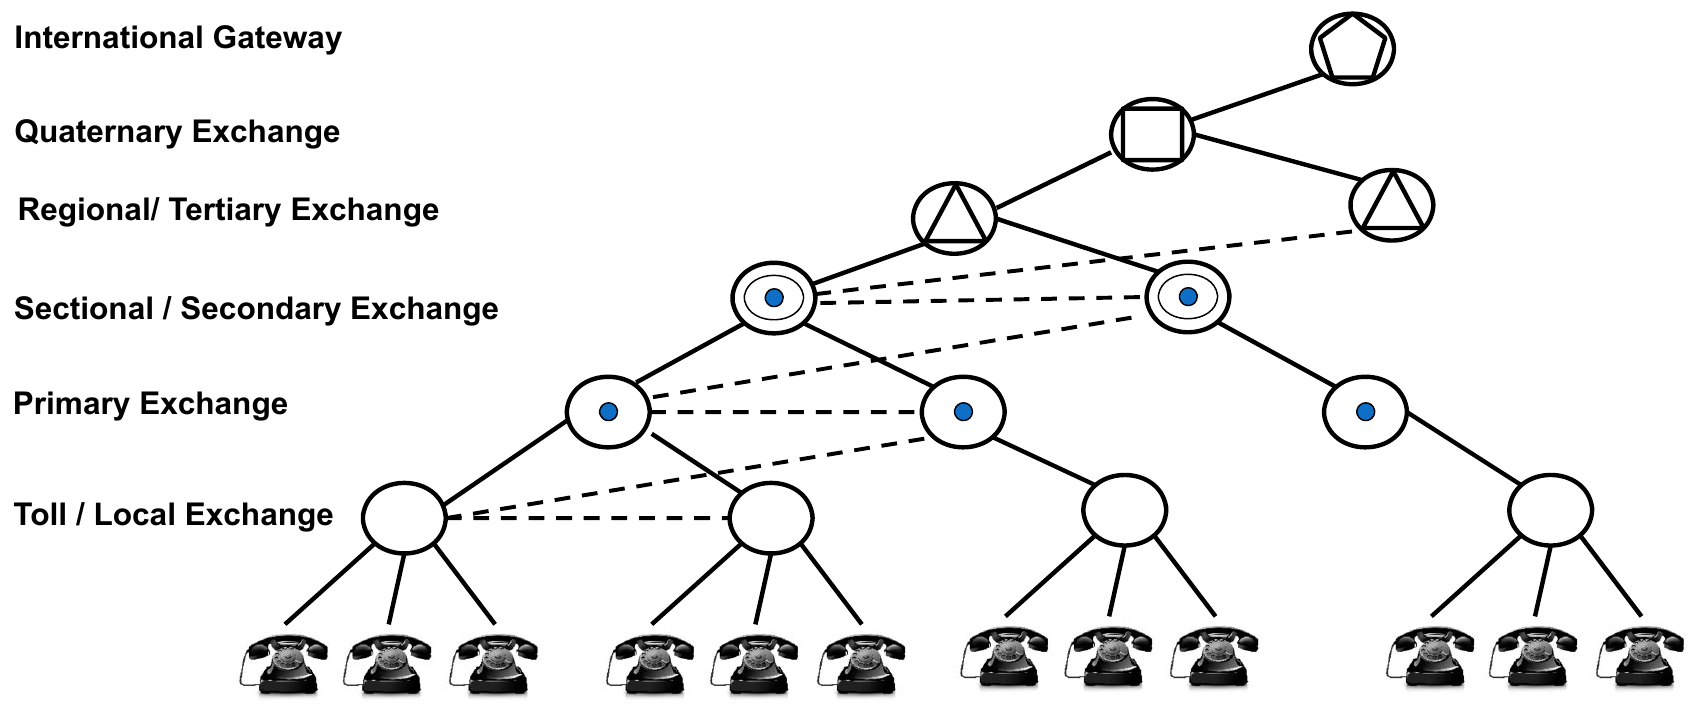
\includegraphics[
		width=14cm,
		%height=15cm
	]{Imágenes/Tema 2/High usage trunks.png}
	\caption{
		\label{fig:unit2_HU}
		High usage trunks
	}
\end{figure}

In very complex urban areas, there are tandem centers that are transit exchanges (without subscribers) connected to other exchanges. These tandem centers are not in the hierarchical network. Once the high usage trunks are present, the path between two subscribers is not unique.

\subsubsection{Routing}

The routing process through high ussage trunks can be decomposed in the following steps:

\begin{enumerate}
	\item Identify the destination tree.
	\item {
		In order to establish the route for the call, at each node I check if there is any high usage trunk (direct section) that brings me to a node in the destination tree and, if it is not congested, I select it. A series of criteria must be followed to select the correct HU:

		\begin{itemize}
			\item If there are several high usage trunks, take the one that brings me nearest.
			\item A route will not ever have two HUs, they can only be used once to reach the destination tree.
			\item {
				The route containing a HU can only have upward normal trunks before HU and downward normal trunks after HU, this is, the routes will always have the shape in figure \ref{fig:unit2_HU_route} or the opposite if it they are done from right to left.

				\begin{figure}[H]
					\centering
					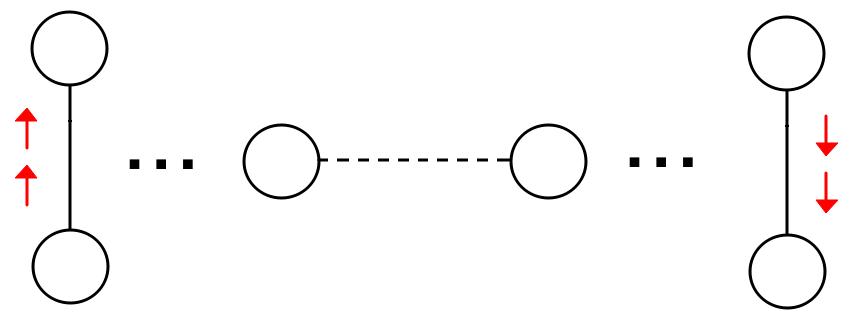
\includegraphics[
						width=7cm,
						%height=15cm
					]{Imágenes/Tema 2/HU.png}
					\caption{
						\label{fig:unit2_HU_route}
						Route containing a HU when going from left to right.
					}
				\end{figure}
			}
		\end{itemize}
	}
	\item If it is congested, I go up in hierarchy, since if any direct section (high usage trunk) has been selected, there is at least another path to the destination. One high usage trunk never overflows to another high usage trunk in the same node. This is, a high usage trunk always overflows to a final trunk. From that, we can establish a corollary: Only one high usage trunk is allowed per path.
	\item Once at the destination tree, we only can descend in hierarchy.
\end{enumerate}

For example, for the network shown in figure \ref{fig:unit2_routing_example}, routes would be:

\begin{itemize}
	\item $A \rightarrow C: AKC, AIKC, AINKC$
	\item $C \rightarrow A: CKA, CKNIA$
	\item $A \rightarrow F: AIPLF, AINLF, AINRPLF$
	\item $F \rightarrow A: FLNIA, FLPIA, FLPRNIA$
\end{itemize}

\begin{figure}[H]
	\centering
	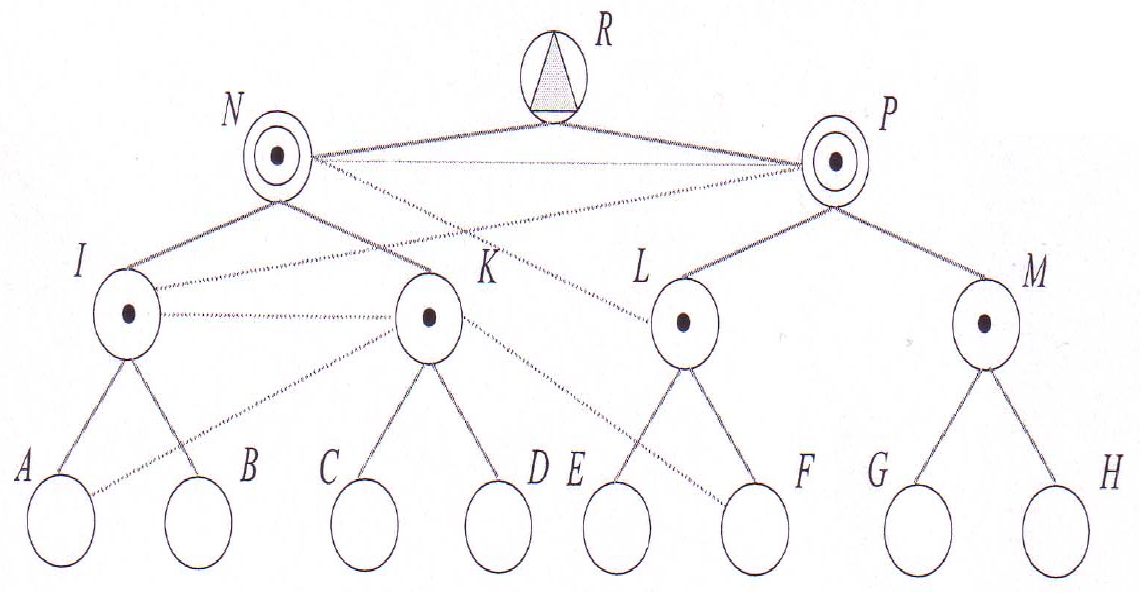
\includegraphics[
		width=10cm,
		%height=15cm
	]{Imágenes/Tema 2/Routing example.png}
	\caption{
		\label{fig:unit2_routing_example}
		Routing example
	}
\end{figure}

\subsubsection{Resultant traffic due to usage HU}

Due to the usage of HU, the resultant traffic both in HU and in FU is complex to estimate. The following scheme presents the different situations we will study:

\iffalse
\begin{tikzpicture}[
  level distance=1.5cm,
  level 1/.style={sibling distance=4cm},
  level 2/.style={sibling distance=2cm},
  level 3/.style={sibling distance=1cm},
  level 4/.style={sibling distance=0.5cm},
  every node/.style={circle,draw}
  ]

% Root node
\node (n1) {1}
% Level 1
  child {node (n2) {2}
    % Level 2
    child {node (n4) {4}
      % Level 3
      child {node (n8) {8}}
      child {node (n9) {9}}
    }
    child {node (n5) {5}
      % Level 3
      child {node (n10) {10}}
      child {node (n11) {11}}
    }
  }
  child {node (n3) {3}
    % Level 2
    child {node (n6) {6}
      % Level 3
      child {node (n12) {12}}
      child {node (n13) {13}}
    }
    child {node (n7) {7}
      % Level 3
      child {node (n14) {14}}
      child {node (n15) {15}}
    }
  };

% Dotted line between nodes 2 and 6
\draw[dotted] (n2) -- (n6);

\end{tikzpicture}
\fi

\begin{figure}[H]
	\centering
	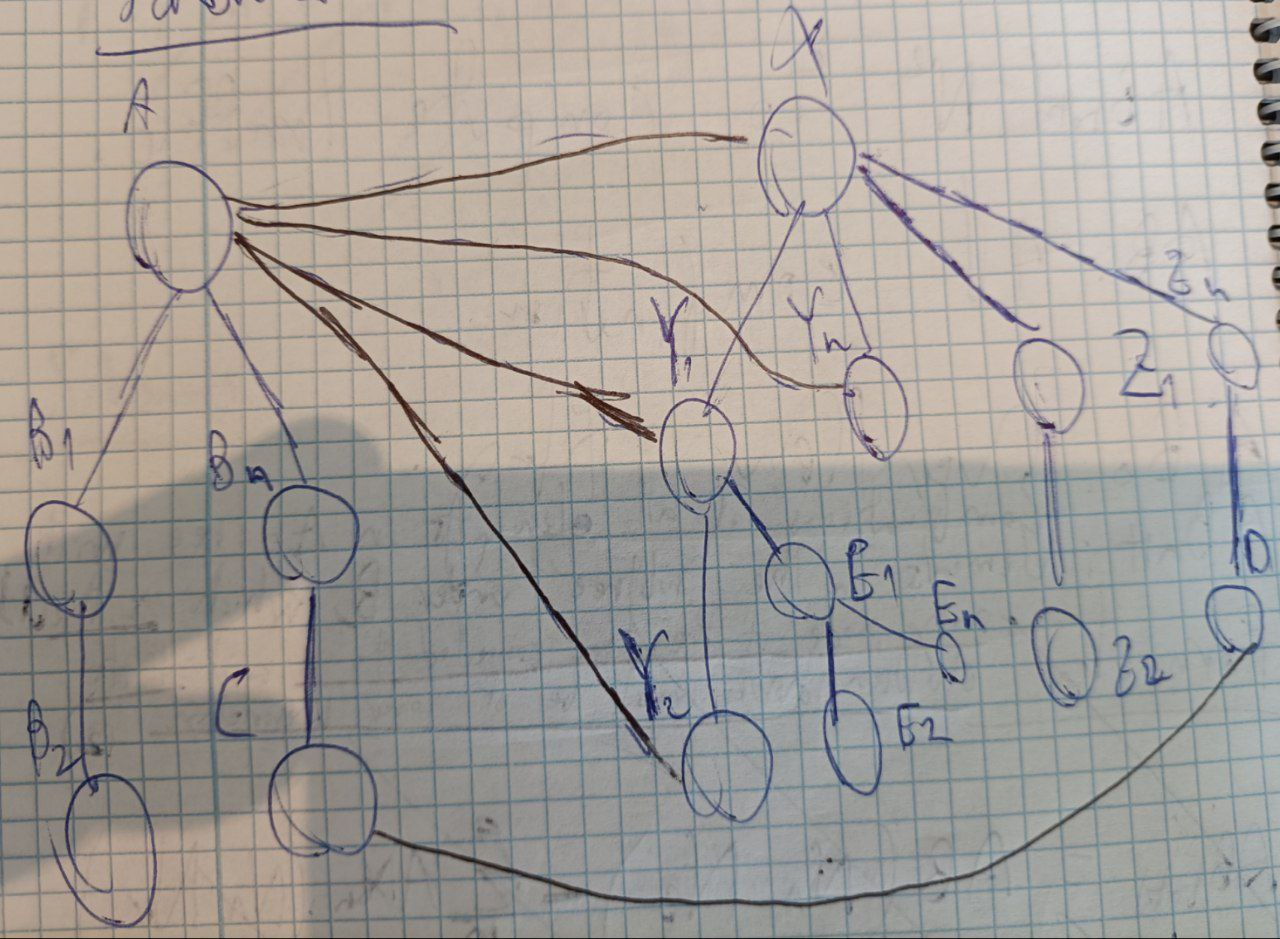
\includegraphics[
		width=12cm,
		%height=15cm
	]{Imágenes/Tema 2/network_scheme.jpg}
	\caption{
		\label{fig:unit2_network_scheme}
		Network scheme.
	}
\end{figure}

Here, in order to study HU between $A$ and $X$ we can distinguish:
\begin{itemize}
	\item Common HU ($AX$): Connects tree $A$ with tree $X$.
	\item Alternative HU ($AY$): Connects tree $A$ with tree $Y$ (a subtree from tree $X$), avoiding traffic going to $AX$.
	\item Lower hierarchy node with no alternative HU ($B$, $Z$): Always sends its traffic to $AX$/$XA$.
	\item Lower hierarchy node with alternative HU ($CD$): Traffic from $C$ to upper $D$ is send to $AX$ always; traffic from $C$ to lower $D$ is sent to $AX$ when saturation in HU.
\end{itemize}

\iffalse
Traffic calculation blablabla:

$$
	OT_{AX} = \sum_{AX} OT_{AX, own} + P_o \cdot \sum_{C, D} OT_{CD}
$$
\fi

In order to obtain the compute traffic at HU or FU we will use a recursive counting method to obtain all the components of the resultant traffic.

\paragraph{Traffic at HU}

The traffic at a HU can be computed in the following steps:
\begin{enumerate}
	\item Add the traffic from each node in tree $A$ to each node in tree $X$.
	\item Subtract the traffic that will be assisted by another HU ($alt$) connected to $A$.
	\item Subtract the traffic that will be assisted by another HU connected to a node from tree $A$, at a lower hierarchy.
	\item Add the traffic resulted by overflow ($o$) of previous HU connected to a node from tree $A$, at a lower hierarchy.
\end{enumerate}

The counting method to obtain the components for calculation will be:

$$
	AX_{total} = AX (N_A \cdot N_X) - \sum_Y AY_{alt} (N_A \cdot N_{YnoA}) + \sum_{C, D} \left( - CD_{alt} + CD_o (1) \right)
$$

Where:

\begin{itemize}
	\item $AX (N_A \cdot N_X) \rightarrow$ Traffic from each node in tree $A$ to each node in tree $X$.
	\item $\sum_Y AY_{alt} (N_A \cdot N_{YnoA}) \rightarrow$ Traffic that will be assisted by another HU connected to $A$.
	\item $\sum_{C, D} CD_{alt} \rightarrow$ Traffic that will be assisted by another HU connected to a node from tree $A$.
	\item $\sum_{C, D} CD_o (1) \rightarrow$ Traffic resulted by overflow of a HU connected to a node from tree $A$.
\end{itemize}

\iffalse
$$
	AX_{total} =
		\underset
			{\text{Traffic from each node in A to each node in B}}
			{\underbrace{AX (N_A \cdot N_X)}}
		\underset
			{\text{Iterations with alternative HUs}}
			{\underbrace{- \sum_Y AY_{alt} (N_A \cdot N_{YnoA})}}
		\underset
			{\text{Iterations with overflowing HUs}}
			{\underbrace{+ \sum_{C, D} \left( - CD_{alt} + CD_o (1) \right)}}
$$
\fi

\paragraph{Traffic at FU}

The traffic at a FU can be computed in the following steps:
\begin{enumerate}
	\item Add the traffic from each node in tree $A$ to each node in tree $X$.
	\item Subtract the traffic that will be assisted by another HU connected to a node from tree $A$.
	\item Add the traffic resulted by overflow ($o$) of previous HU connected to a node from tree $A$.
\end{enumerate}

The counting method to obtain the components for calculation will be:

$$
	AX_{total} = AX (N_A \cdot N_X) + \sum_{C, D} \left( - CD_{alt} + CD_o (1) \right)
$$

Where:

\begin{itemize}
	\item $AX (N_A \cdot N_X) \rightarrow$ Traffic from each node in tree $A$ to each node in tree $X$.
	\item $\sum_{C, D} CD_{alt} \rightarrow$ Traffic that will be assisted by another HU connected to a node from tree $A$.
	\item $\sum_{C, D} CD_o (1) \rightarrow$ Traffic resulted by overflow of a HU connected to a node from tree $A$.
\end{itemize}

\iffalse
$$
	AX_{total} =
		\underset
			{\text{Traffic from each node in A to each node in B}}
			{\underbrace{AX (N_A \cdot N_X)}}
		\underset
			{\text{Iterations with overflowing HUs}}
			{\underbrace{+ \sum_{C, D} \left( - CD_{alt} + CD_o (1) \right)}}
$$
\fi

\paragraph{Notation in counting methods}

\begin{itemize}
	\item $AB_{total}$: Number of elements to compute traffic in the HU that connects $A$ and $B$.
	\item $AB$: Size of the set with all the combinations of elements from $A$ tree and $B$ tree.
	\item $AB_o$: Element that indicates the traffic resulting from overflow in the HU that connects $A$ and $B$.
	\item {
		$AB_{alt}$: Combinations of all elements in tree $A$ with elements in the limited subtree under $B$. The limited subtree under $B$ is defined by:
		\begin{itemize}
			\item $B$ is the only node of the tree connected to $A$.
			\item All its children nodes must be of lower hierarchy.
		\end{itemize}
	}
	\item {
		$AB_{alt}$: \textbf{Independent} combinations of elements in tree $A$ with elements in the limited subtree $B$ to compute the traffic in the HU between $A$ and $B$.
	}
\end{itemize}

The following relation can be useful:

\begin{itemize}
	\item $\sum_Y AY_{alt} (N_A \cdot N_{YnoA}) = AY_{highest} (N_A \cdot N_{Y_{highest}})$
	\item $N_{YnoA} = 1 + N_E$
\end{itemize}

\subsubsection{Concepts}

Two important concepts arise from the networks scenario:

\begin{itemize}
	\item {
		\textbf{Bid}

		Bid is the attempt to establish a conversation:

		\begin{itemize}
			\item Lifting a telephone.
			\item Partial dialing.
			\item Complete dialing, get the engage tone.
			\item Get ring tone back, no answer.
			\item Get ring tone back, answer.
		\end{itemize}

		Bids are the number of calls seized the circuits plus the number of calls rejected due to all circuits are busy assuming that there are no switching congestion.
	}
	\item {
		\textbf{Seizure}

		A seizure is a bid from d. It can be rejected or answered. Seizures are the number of calls answered plus the number of calls unanswered plus number of calls to busy plus subscribers plus the number of calls to recorded announcements.
	}
\end{itemize}

We can establish the following relation:

$$
	Bids > Seizures > Answers
$$

\subsection{Intelligent network}

\subsubsection{Introduction}

The concept of intelligent network was originated after digitalization and at the same time of ISDN. The first standards were established in 1992 by CCITT (now UIT-T): Q.1200.

It offer added value services:

\begin{itemize}
	\item Routing and number translations.
	\item Virtual Private Networks (VPNs).
	\item Special billing.
	\item Operator oriented services.
\end{itemize}

\subsubsection{Architecture}

We must distinguish the following elements:

\begin{itemize}
	\item Service Switching Point (SSP): It catches or switches service requests by triggers such as prefixes.
	\item Signalling Transfer Point (STP): It interchanges signaling information among different points in the telephony network.
	\item Service Control Point (SCP): It is a stand alone computer connected to a database. It knows what to do with each service.
	\item External Data Base (DB): The SCP might need to use an external data base for certain services. For example, a credit card data base.
	\item Adjunct: Same functions as SCP but referred to a local exchange.
	\item {
		Intelligent Peripheral (IP): It has several functions:
		\begin{itemize}
			\item Voice synthesis, either from already stored text messages or text to voice conversion.
			\item Voice recognition that allows users to answer questions or select options (numbers, yes or no, ...).
			\item Voice recording such as voice mailbox.
			\item Multi-frequency digit recognition at second dialing phase.
		\end{itemize}
	}
	\item Service Management System (SMS): Gives complete and secure information to each SCP (sink for statistical data, service measurements, alarms, ...). Technical and commercial management for intelligent network. It does not need real time connections.
	\item {
		Service Creation Environment Point (SCE/P): It helps in the creation of new services through several stages:
		\begin{itemize}
			\item {
				Formal service specification:
				\begin{itemize}
					\item Service development.
					\item Service verification.
					\item Service simulation.
				\end{itemize}
			}
			\item Service implantation.
		\end{itemize}
	}
\end{itemize}

\begin{figure}[H]
	\centering
	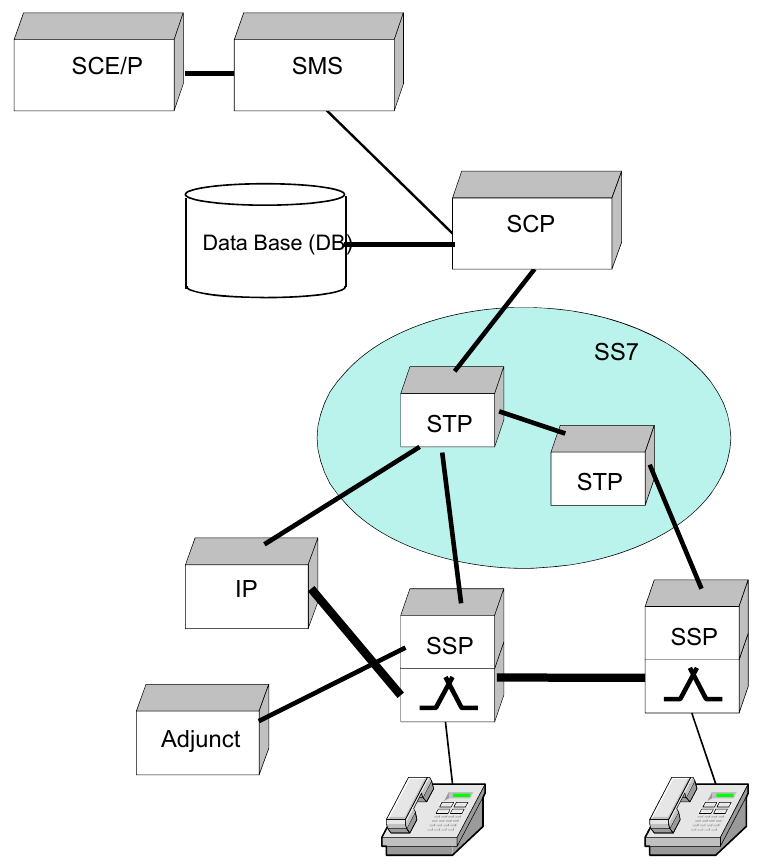
\includegraphics[
		width=12cm,
		%height=15cm
	]{Imágenes/Tema 2/Intelligent network.png}
	\caption{
		\label{fig:unit2_int_net}
		Intelligent network scheme
	}
\end{figure}

\section{Multiplexing and multiple access}

\subsection{Introduction}

The study of multiplexing and multiple access requires the following parameters:

\begin{itemize}
	\item Offered traffic from users ($I$).
	\item Retransmissions ($R$): It is the traffic resulted from retransmissions.
	\item {
		Offered traffic to the net ($G$):

		$G = I + R$
	}
	\item {
		Network efficiency ($S$): It can be computed from offered traffic to the net in relation with offered traffic from users and retransmissions:

		$S = S(G, I , R)$

		If there is no congestion, it equals offered traffic:

		$S \overset{\mathrm{(no \quad congestion)}}{=} I$

		Previous measures can be normalized to network efficiency $S$, so instead of Erlangs, they will be packets (transmissions) per packet:

		$\overline{I} = \frac {I} {S} \overset{\mathrm{(no \quad congestion)}}{=} 1$

		$\overline{R} = \frac {R} {S}$

		$\overline{G} = \frac {G} {S} = \overline{I} + \overline{R} = \frac {I + R} {S}$
	}
	\item {
		Packet propagation: It is the normalized propagation time ($t_p$). So:

		$a = \frac {t_p} {W_s}$
	}
	\item {
		Generating acknowledgement: It is the normalized acknowledgement time ($t_{ACK}$). So:

		$w = \frac {t_{ACK}} {W_s}$
	}
	\item {
		Transmission delay: It is the normalized delay. So:

		$D = \frac {t_{tx}} {W_s}$
	}
\end{itemize}

\begin{figure}[H]
	\centering
	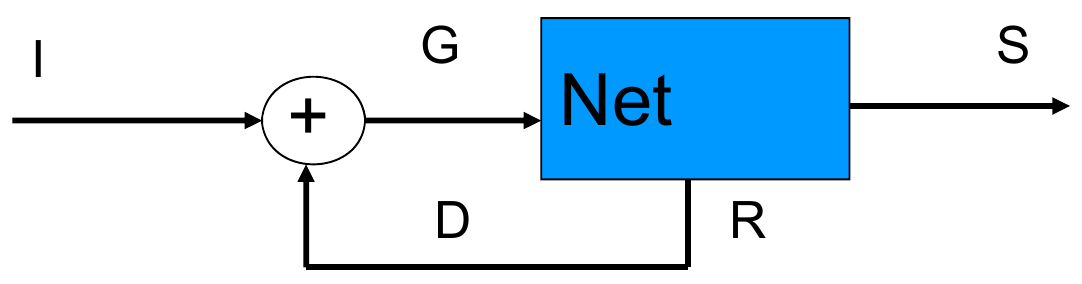
\includegraphics[
		width=10cm,
		%height=15cm
	]{Imágenes/Tema 2/Multiplexing and multiple access.png}
	\caption{
		\label{fig:unit2_mul}
		Scheme of network traffic
	}
\end{figure}

To solve multiplexing and multiple access problem, several access protocols have been developed.

\subsection{Centralized Aloha}

It was invented at the Hawaii University in 1970. There is a distributed variant, but since packet propagation ($a$) is usually small, the centralized version is commonly used for both scenarios.

Its operation can be summarized in:

\begin{itemize}
	\item If the terminal wants to transmit, it does and waits for the acknowledgement.
	\item If the acknowledgement is not received, it retransmits waiting a random time between $1$ and $k$.
\end{itemize}

\begin{figure}[H]
	\centering
	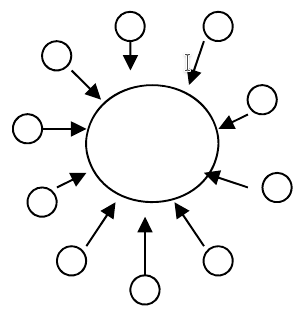
\includegraphics[
		width=5cm,
		%height=15cm
	]{Imágenes/Tema 2/Centralized.png}
	\caption{
		\label{fig:unit2_cen_aloha_sheme}
		Centralized Aloha scheme
	}
\end{figure}

Its characteristics are:

\begin{itemize}
	\item {
		Transmission delay:

		$
			D =
			\left( \frac {G} {S} - 1 \right) \cdot \left( \frac {k+1} {2} + 1 + 2a + w \right) + a + 1 \overset{\frac {G} {S} = e^{2G}}{=}
			\left( e^{2G} - 1 \right) \cdot \left( \frac {k+1} {2} + 1 + 2a + w \right) + a + 1
		$
	}
	\item {
		Network efficiency: Assuming Poisson arrivals, we have:

		$
			S = G \cdot e^{-2G}
		$

		Its maximum value, for $G = 0.5$ is:

		$
			S_{MAX} = 0.5 e^{-1} = 0.184
		$
	}
\end{itemize}

\begin{figure}[H]
	\centering
	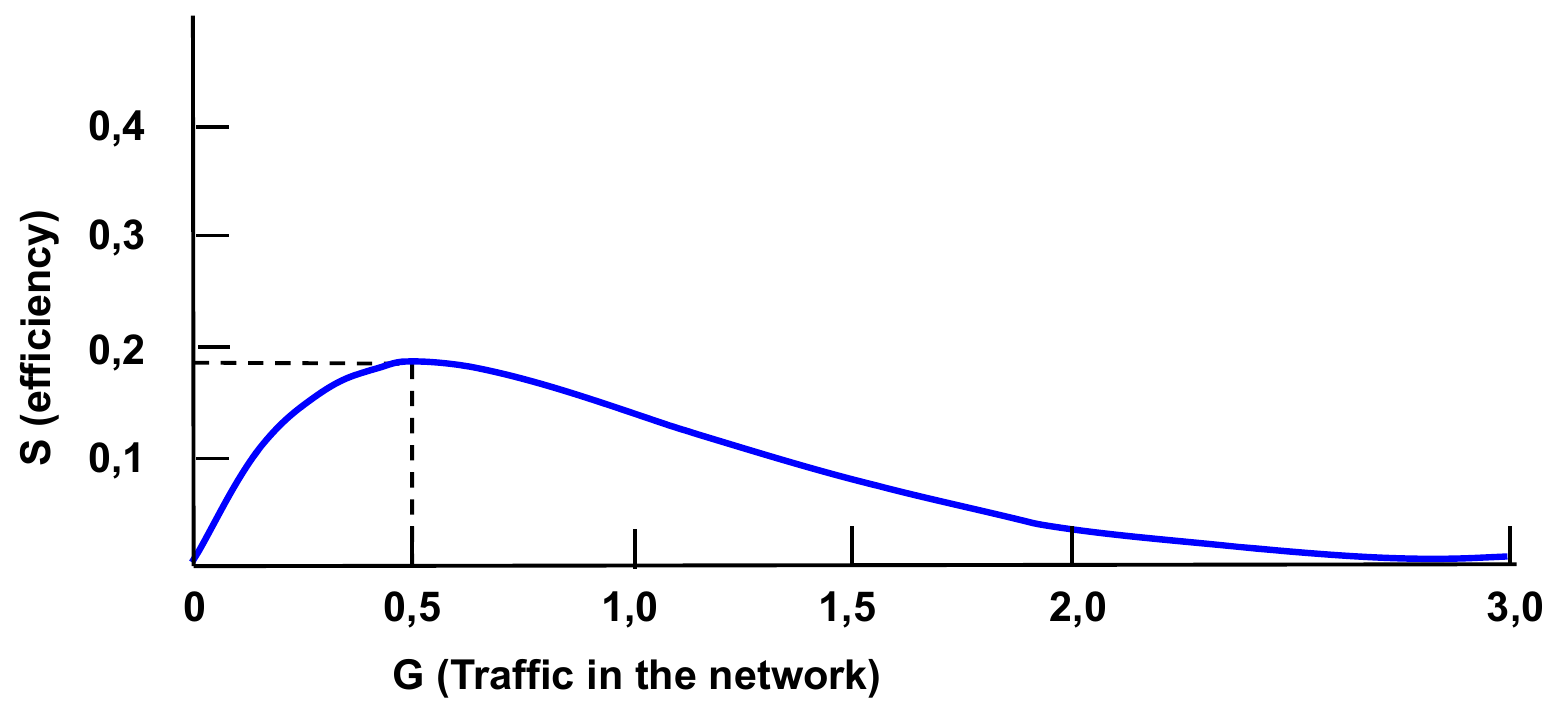
\includegraphics[
		width=12cm,
		%height=15cm
	]{Imágenes/Tema 2/Centralized Aloha S.png}
	\caption{
		\label{fig:unit2_cen_aloha_S}
		Centralized Aloha efficiency
	}
\end{figure}

\subsection{Distributed Aloha}

\begin{figure}[H]
	\centering
	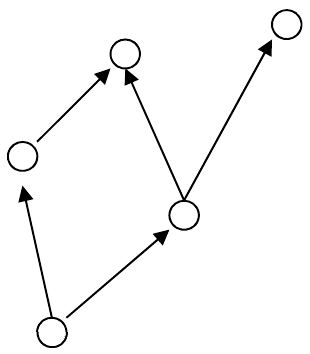
\includegraphics[
		width=5cm,
		%height=15cm
	]{Imágenes/Tema 2/Distributed.png}
	\caption{
		\label{fig:unit2_dis_aloha_sheme}
		Distributed Aloha scheme
	}
\end{figure}

It is distributed. Its characteristics are:

\begin{itemize}
	\item {
		Transmission delay:

		$
			D =
			\left( \frac {G} {S} - 1 \right) \cdot \left( \frac {k+1} {2} + 1 + 2a + w \right) + a + 1 \overset{\frac {G} {S} = e^{2G \cdot (1+a)}}{=}
			\left( e^{2G \cdot (1+a)} - 1 \right) \cdot \left( \frac {k+1} {2} + 1 + 2a + w \right) + a + 1
		$
	}
	\item {
		Network efficiency: Assuming Poisson arrivals, we have:

		$
			S = G \cdot e^{-2G \cdot (1+a)}
		$
	}
\end{itemize}

\subsection{Slotted Aloha}

It is an improvement on simple Aloha to solve collisions problem. Its operation can be summarized in:

\begin{itemize}
	\item The time is divided into slots.
	\item Only transmission at the beginning of the slots is allowed.
\end{itemize}

\begin{figure}[H]
	\centering
	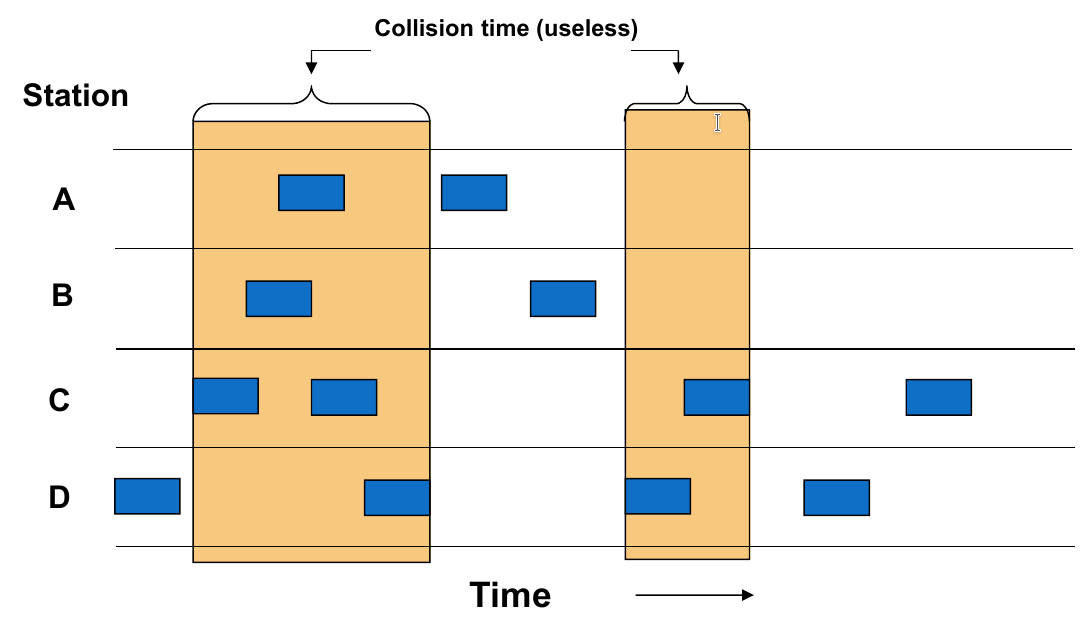
\includegraphics[
		width=14cm,
		%height=15cm
	]{Imágenes/Tema 2/Slotted Aloha.png}
	\caption{
		\label{fig:unit2_slo_aloha_sheme}
		Slotted Aloha scheme
	}
\end{figure}

Its characteristics are:

\begin{itemize}
	\item {
		Packet propagation: It is the normalized propagation time ($t_p$). So:

		$
			a = \frac {t_p} {W_s}
		$
	}
	\item {
		Generating acknowledgement: It is the normalized acknowledgement time ($t_{ACK}$). So:

		$
			w = \frac {t_{ACK}} {W_s}
		$
	}
	\item {
		Transmission delay:

		$
			D =
			\left( \frac {G} {S} - 1 \right) \cdot \left( \frac {k+1} {2} + 1.5 + 2a + w \right) + a + 1.5 \overset{\frac {G} {S} = e^G}{=}
			\left( e^G - 1 \right) \cdot \left( \frac {k+1} {2} + 1.5 + 2a + w \right) + a + 1.5
		$
	}
	\item {
		Offered traffic to the net:

		$
			G = S + R
		$
	}
	\item {
		Network efficiency: Assuming Poisson arrivals, we have:

		$
			S = G \cdot e^{-G}
		$

		Its maximum value, for $G = 1$, is:

		$
			S_{MAX} = e^{-1} = 0.368
		$
	}
\end{itemize}

\begin{figure}[H]
	\centering
	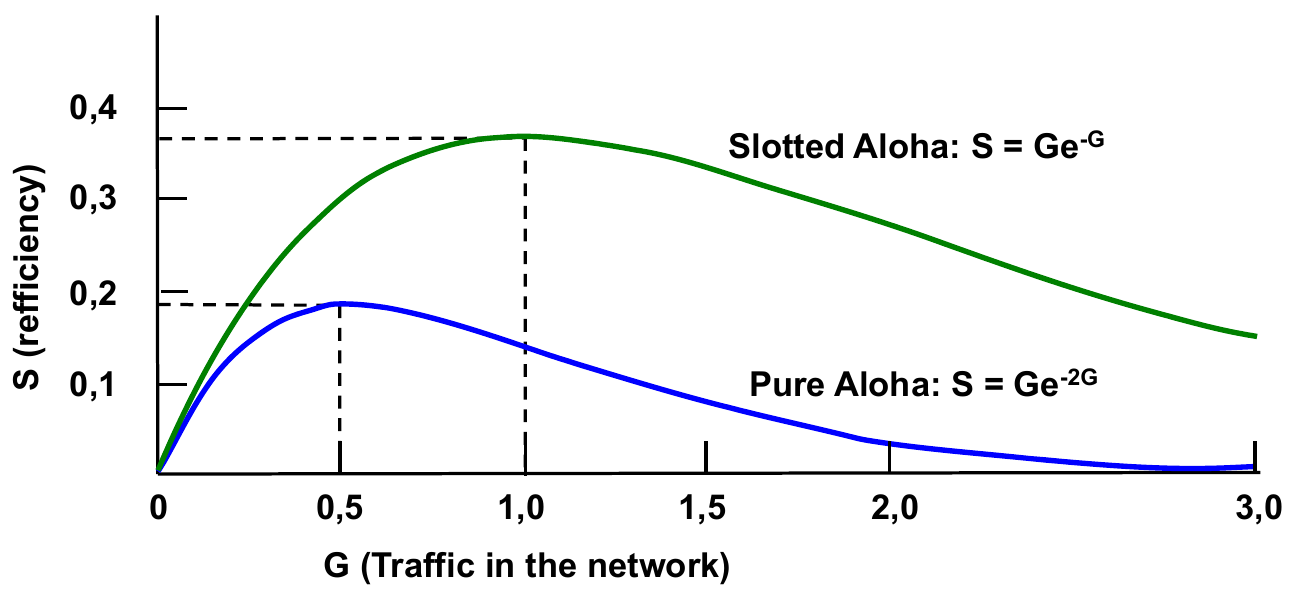
\includegraphics[
		width=12cm,
		%height=15cm
	]{Imágenes/Tema 2/Aloha comparison.png}
	\caption{
		\label{fig:unit2_aloha_comp}
		Aloha comparison
	}
\end{figure}

\subsection{Carrier Sense Multiple Access (CSMA)}

Before transmission, the channel is sensed:

\begin{itemize}
	\item Before transmitting, channel is listen.
	\item If no one is transmitting, it transmits.
	\item {
		If the channel is busy:
		\begin{itemize}
			\item {
				Non-persistent: It waits a random time and then, the process starts.

				$
					S = \frac {G} {G+1}
				$
			}
			\item {
				1-persistent: It waits until the channel is free and it transmits once it is. If collision, again 1-persistent.

				$
					S = \frac {G \cdot (1 + G) \cdot e^{-G}} {G + e^{-G}}
				$

				$
					S_{MAX} = 0.55
				$
			}
			\item $p$-persistent: It waits with probability $1 - p$ and transmits with probability $p$.
		\end{itemize}
	}
\end{itemize}

\begin{figure}[H]
	\centering
	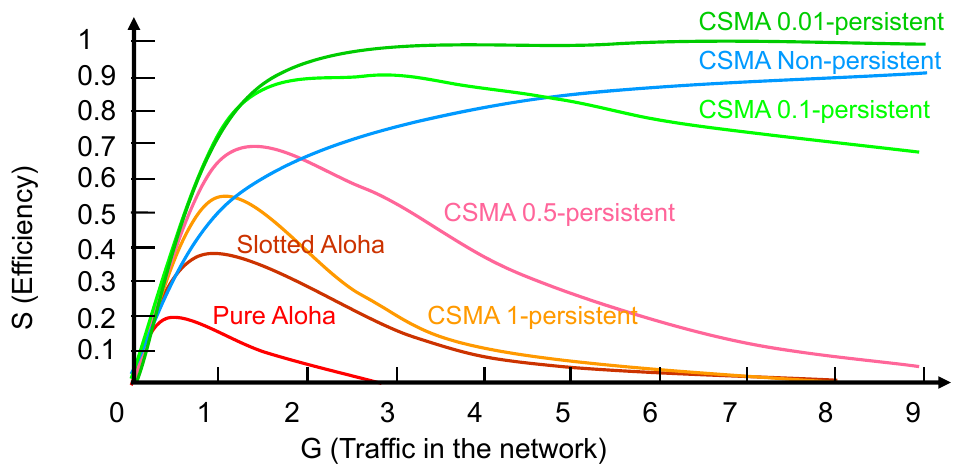
\includegraphics[
		width=12cm,
		%height=15cm
	]{Imágenes/Tema 2/All comparison.png}
	\caption{
		\label{fig:unit2_all_comp}
		Comparison of all transmission protocols
	}
\end{figure}

\subsubsection{Summary}

\begin{tabular}{|c|c|c|}
	\hline
	& $S$ & $S_{MAX}$ \\
	\hline
	Aloha & $G \cdot e^{-2G}$ & $0.5 e^{-1} = 0.184$ \\
	\hline
	Distributed Aloha & $G \cdot e^{-2G \cdot (1+a)}$ & \\
	\hline
	Slotted Aloha & $G \cdot e^{-G}$ & $e^{-1} = 0.368$ \\
	\hline
	CSMA (Non-persistent) & $\frac {G} {G+1}$ & \\
	\hline
	CSMA (1-persistent) & $\frac {G \cdot (1 + G) \cdot e^{-G}} {G + e^{-G}}$ & $0.55$ \\
	\hline
	CSMA ($p$-persistent) & & \\
	\hline
\end{tabular}

\begin{landscape}

\begin{tabular}{|c|c|}
	\hline
	& $D$ \\
	\hline
	Aloha & $\left( \frac {G} {S} - 1 \right) \cdot \left( \frac {k+1} {2} + 1 + 2a + w \right) + a + 1 \overset{\frac {G} {S} = e^{2G}}{=} \left( e^{2G} - 1 \right) \cdot \left( \frac {k+1} {2} + 1 + 2a + w \right) + a + 1$ \\
	\hline
	Distributed Aloha & $\left( \frac {G} {S} - 1 \right) \cdot \left( \frac {k+1} {2} + 1 + 2a + w \right) + a + 1 \overset{\frac {G} {S} = e^{2G \cdot (1+a)}}{=} \left( e^{2G \cdot (1+a)} - 1 \right) \cdot \left( \frac {k+1} {2} + 1 + 2a + w \right) + a + 1$ \\
	\hline
	Slotted Aloha & $\left( \frac {G} {S} - 1 \right) \cdot \left( \frac {k+1} {2} + 1.5 + 2a + w \right) + a + 1.5 \overset{\frac {G} {S} = e^G}{=} \left( e^G - 1 \right) \cdot \left( \frac {k+1} {2} + 1.5 + 2a + w \right) + a + 1.5$ \\
	\hline
	CSMA (Non-persistent) & \\
	\hline
	CSMA (1-persistent) & \\
	\hline
	CSMA ($p$-persistent) & \\
	\hline
\end{tabular}

\end{landscape}

\section{Link budget and transmission}

\subsection{Power and decibels}

\subsubsection{Definition}

Decibels are always obtained from a relation:

$$
	c = \frac {a} {b} \rightarrow c_{dB} = 10 \log (c) = 10 \log \left( \frac {a} {b} \right) = 10 \log (a) - 10 \log (b) = a_{dB} - b_{dB}
$$

They are commonly used to represent concepts related to power since they usually imply two quatities we can relate. For example, gains and losses (power of a signal before and after transmission).

\subsubsection{Reference and conversion}

Absolute values need a reference:

\begin{itemize}
	\item $dBW$: Referred to Watts ($W$)
	\item $dBm$: Referred to $mW$
	\item $dB\mu$: Referred to $\mu W$
\end{itemize}

Since the relation between them is an order of 3 ($30 dB$), we can convert between them by adding and subtracting $30 dB$.

\begin{figure}[H]
	\centering
	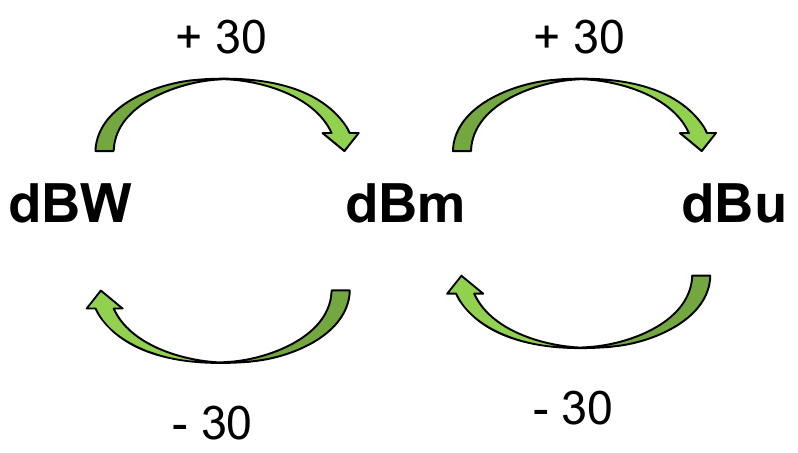
\includegraphics[
		width=6cm,
		%height=15cm
	]{Imágenes/Tema 2/Decibels conversion.png}
	\caption{
		\label{fig:unit2_dedibels}
		Decibels conversion
	}
\end{figure}

\subsection{Gains and losses}

When a signal is transmitted ($p_{tx}$), it can be amplified with a certain gain ($g$) or suffer losses ($l$). The resulting power ($p_{rx}$) is the product by gains and division by losses:

$$
	p_{rx} = p_{tx} \cdot \frac {\prod_i g_i} {\prod_i l_i}
$$

It is usually expressed in decibels:

$$
	P_{rx} = T_{tx} + \sum_i G_i - \sum_j L_j
$$

Where:

\begin{itemize}
	\item $P_{tx} = 10 \log (p_{tx})$
	\item $P_{rx} = 10 \log (p_{rx})$
	\item $G_i = 10 \log (g_i)$
	\item $L_i = 10 \log (l_i)$
\end{itemize}

\subsection{Propagation}

\subsubsection{Total propagation losses (in decibels)}

$$
	l_b = l_{bf} \cdot a_E
$$

$$
	L_b = L_{bf} + A_E
$$

Where:

\begin{itemize}
	\item Free-space path loss: $l_{bf}$
	\item Losses due to other factors: $a_E$
\end{itemize}

\subsubsection{Free-space path loss}

$$
	l_{bf} = \left( \frac {4 \pi d} {\lambda} \right)^2
$$

$$
	L_{bf} = 10 \log \left[ \left( \frac {4 \pi d} {\lambda} \right)^2 \right]
$$

Where:

\begin{itemize}
	\item Distance to antenna: $d$
	\item Wavelength: $\lambda$
\end{itemize}

\subsubsection{Free-space path loss (variable index)}

$$
	l_{bf} = \left( \frac {4 \pi d} {\lambda} \right)^n
$$

$$
	L_{bf} = 10 \log \left[ \left( \frac {4 \pi d} {\lambda} \right)^n \right]
$$

Where:

\begin{itemize}
	\item Distance to antenna: $d$
	\item Wavelength: $\lambda$
	\item Propagation index: $n$
\end{itemize}

\subsubsection{Antenna gain}

$$
	g = \eta \left( \frac {\pi D} {\lambda} \right)^2
$$

$$
	G = 10 \log \left[ \eta \left( \frac {\pi D} {\lambda} \right)^2 \right]
$$

Where:

\begin{itemize}
	\item Antenna diameter: $D$
	\item Wavelength: $\lambda$
	\item Antenna efficiency: $\eta$
\end{itemize}

\subsection{Interference}

\subsubsection{Noise power spectral density (adjusted to bandwidth)}

$$
	p_N = N = N_0 B = k T_0 B
$$

$$
	P_N = N_{dB} = 10 \log (N_0) + 10 \log (B) = 10 \log (k T_0 B)
$$

Where:

\begin{itemize}
	\item Boltzman constant: $k = 1.38 \cdot 10^{-23} [J/K]$
	\item Receiver system noise temperature in kelvins: $T_0$
	\item Channel bandwidth: $B$
\end{itemize}

\subsubsection{Carrier-to-noise ratio}

$$
	\left( \frac {C} {N} \right) = \frac {p_{rx}} {k T_0 B}
$$

$$
	\left( \frac {C} {N} \right)_{dB} = P_{rx} + 10 \log \left( \frac {1} {T_0} \right) - 10 \log (k B)
$$

Where:

\begin{itemize}
	\item Boltzman constant: $k = 1.38 \cdot 10^{-23} [J/K]$
	\item Receiver system noise temperature in kelvins: $T_0$
	\item Noise power spectral density: $N_0$
	\item Noise power spectral density (adjusted to bandwidth): $N$
	\item Carrier signal average power: $C$
	\item Channel bandwidth: $B$
	\item Data rate: $R_b$
\end{itemize}

\subsubsection{Energy per bit to noise ratio}

$$
	\frac {E_b} {N_0} = \frac {C} {N} \frac {B} {R_b} = \frac {C} {N_0} \frac {1} {R_b}
$$

Where:

\begin{itemize}
	\item Energy per bit: $E_b$
	\item Noise power spectral density: $N_0$
	\item Noise power spectral density (adjusted to bandwidth): $N$
	\item Carrier signal average power: $C$
	\item Channel bandwidth: $B$
	\item Data rate: $R_b$
\end{itemize}

\chapter{Broadband fixed systems}

\section{Introduction}

Transmitted data through networks has increassed in last decade. Networks, originally focused on voice, now are moving to multimedia and interactive services, resulting in a set of new requirements:

\begin{itemize}
	\item Efficient use of bandwidth, which is highly demanded.
	\item Flexibility for changing services and usage.
	\item Achievement of coverage for all digital service, also known as "one network for everything" (B-ISDN).
\end{itemize}

For that purpose, there have been developed flexible network architectures for access and transport:

\begin{itemize}
	\item Integrated Services Digital Network (ISDN).
	\item Digital Subscriber Line (DSL).
	\item Synchronous Digital Hierarchy (SDH) / Synchronous Optical NETwork (SONET).
	\item Dense Wavelength Division Multiplexing ((D)WDM).
	\item Asynchronous Transfer Mode (ATM).
	\item {
		Wireless systems:
		\begin{itemize}
			\item Multichannel Multipoint Distribution Service (MMDS).
			\item Local Multipoint Distribution Service (LMDS).
			\item Wireless Local Area Networks (WLAN).
			\item Worldwide Interoperability for Microwave Access (WiMAX).
		\end{itemize}
	}
\end{itemize}

Those architectures can be classified in two kinds of complementary networks:

\begin{itemize}
	\item Access Networks: They allow the service operator to give users the access to services, this is, they are managed and perform terminal communications activities. Some examples are ISDN, PSTN, xDSL and WiFi.
	\item Core Networks (also called Transport Networks): High capacity networks to interconnect other networks such as the access networks, this is, they are unmanaged and perform intermediate communications activities. Some examples are SDH, ATM, (D)WDM and IP.
\end{itemize}

The implementation of these systems still must face some limitations:

\begin{itemize}
	\item Congestion due to bandwidth limitation.
	\item Adaptation to new users requirements, like data type (video, multimedia, etc.) and service (P2P, instantaneous digital communicarion, etc.).
\end{itemize}

Previous to current technology, Plesiochronous Digital Hierarchy (PDH) was a standard with the following specifications:

\begin{itemize}
	\item Time Division Multiplexing (TDM).
	\item European PDH: 30 channel (E1) at $64 kbps$ (E0). Hierarchy up to E4.
	\item American PDH: 24 channels (T1) at $64 kbps$ (T0) (two of them at $56 kbps$).
\end{itemize}

\section{Integrated Services Digital Network (ISDN)}

\subsection{Introduction}

ISDN provides the standards for a network that is able to carry different types of information (voice, data, texts, images, ...) in digital format and end to end. It is an evolution from telephony Integrated Digital Network (IDN), so it offers connections up to $64 kbps$ by circuit switching and also packet switching services are allowed. It provides an integrated subscriber access. Its evolution comprises:

\begin{itemize}
	\item {
		N-ISDN:
		\begin{itemize}
			\item Connection up to $64 kbps$.
			\item Connection up to $n \times 64 kbps$ ($< 2 Mbps$).
		\end{itemize}
	}
	\item B-ISDN: Connections above $2 Mbps$.
\end{itemize}

\subsection{Reference configuration}

ISDN's goal is to use a reduced set of interfaces between user and network for low cost and to hold a large number of applications, equipments and configurations. Terminals are:

\begin{itemize}
	\item R: It connects terminal equipment with terminal adapters: TE - TA.
	\item S: It connects terminal equipment with network terminations and terminal adapters with network terminations: TE - NT, TA - NT.
	\item T: It connects terminal equipment with network terminations, terminal adapters with network terminations and network terminations with other network terminations: TE - NT, TA - NT, NT - NT.
	\item U: It connects network terminations with line terminations: NT - LT.
	\item V: It connects line terminations with exchange terminations: LT - ET.
\end{itemize}

\begin{figure}[H]
	\centering
	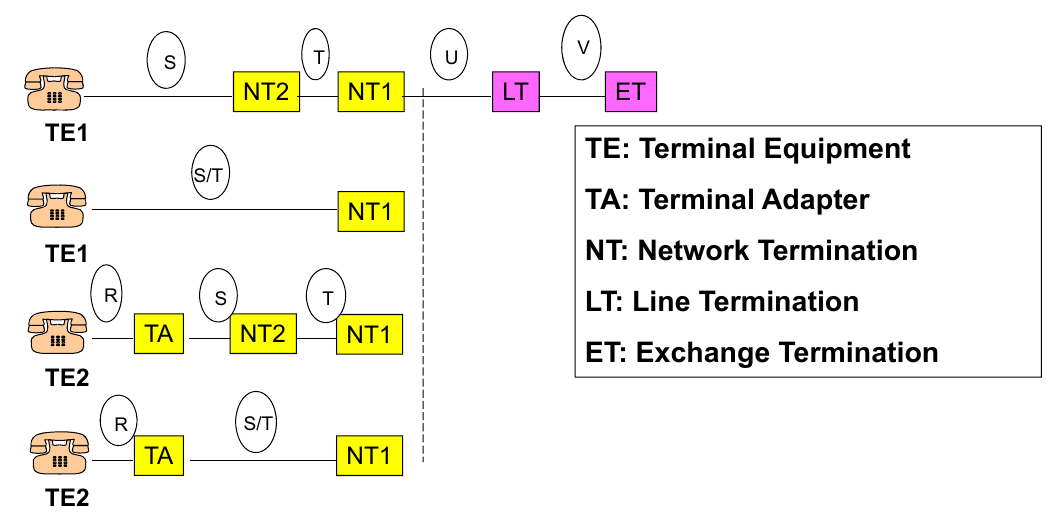
\includegraphics[
		width=12cm,
		%height=15cm
	]{Imágenes/Tema 3/Reference configuration.png}
	\caption{
		\label{fig:unit3_ref_conf}
		ISDN reference configuration
	}
\end{figure}

\subsection{Channels}

ISDN establishes different types of data channel whose implementation is done at bit level, inside data frames. There are three types:

\begin{itemize}
	\item Channel B: Used to transport data (including voice). Its data rate is 64 kbps.
	\item Channel D: Used for signaling (low data rate). Its data rate can be 16 kbps or 64 kbps.
	\item {
		Channel H: Used to transport data. Its data rate is higher than 64 kbps. The are three types:
		\begin{itemize}
			\item H0: Its data rate can be 384 kbps or 375 kbps (6 channels B).
			\item H11: Its data rate can be 1536 kbps or 1500 kbps (24 channels B). It is used in countries with DS1 (1544 kbps) hierarchy.
			\item H12: Its data rate can be 1920 kbps or 1875 kbps (30 channels B). It is used in countries with E1 (2048 kbps) hierarchy.
		\end{itemize}
	}
\end{itemize}

\subsection{Transmission}

For transmission, we use several channels multiplexed in TDM (frame). For each purpose:

\begin{itemize}
	\item Voice transmission and 3.1 kHz digital audio. 8 bits each, 125 $\mu$s (64 kbps).
	\item Data transmission. Several data rates adapted to 64 kbps.
	\item {
		Signaling:
		\begin{itemize}
			\item Data rate up to 16 kbps or 64 kbps.
			\item It is fixed in the frame, but it can be used for data in certain cases.
		\end{itemize}
	}
\end{itemize}

\subsection{Access type}

There are two access types, basic rate and primary rate, which will be able to work in specific interfaces.

\subsubsection{Basic rate}

The useful data rate is calculated in the following way:

$$
	2B + D = 2 \times 64 kbps + 16 kbps = 144 kbps
$$

It can be supported by almost all current at 2W by using duplex digital multiplex transmission (echoes cancellation). The main application is residential or small offices with few terminals. We distinguish two types depending on the interface:

\begin{itemize}
	\item {
		At S interface:
		\begin{itemize}
			\item The data rate is 192 kbps.
			\item {
				The frame:
				\begin{itemize}
					\item Frames have 48 bits ($L = 48 [b] $) and they are transmitted in 250 microseconds ($T_{tx} = 250 [\mu s/frame]$), resulting in 4000 frames per second ($f_{tx} = 1/T_{tx} = 4000 [frames/s]$) or 192 kbps ($C = f_{tx} \cdot L = 192 [kbps]$).
					\item Each channel B is divided in two groups of slots, B1 and B2.
					\item Each channel B group is composed by two 8-bit slots, resulting in four 8-bit slots.
					\item The channel B slots sent alternatively and between each channel B slot one channel D slot (1 bit) is inserted, resulting in 36 bits.
					\item Only 36 useful bits of 48.
					\item {
						One single channel B group rate:

						$
							\frac {2 \cdot 8 [b]} {250 \cdot 10^{-6} [s]} = 64 \cdot 10^3 [bps]
						$
					}
					\item {
						B channel rate:

						$
							\frac {4 \cdot 8 [b]} {250 \cdot 10^{-6} [s]} = 128 \cdot 10^3 [bps]
						$
					}
					\item {
						D channel rate:

						$
							\frac {4 \cdot 1 [b]} {250 \cdot 10^{-6} [s]} = 16 \cdot 10^3 [bps]
						$
					}
					\item {
						Total rate:

						$
							\frac {4 \cdot 8 [b] + 4 \cdot 1 [b]} {250 \cdot 10^{-6} [s]} = 144 \cdot 10^3 [bps]
						$
					}
				\end{itemize}

				\begin{figure}[H]
					\centering
					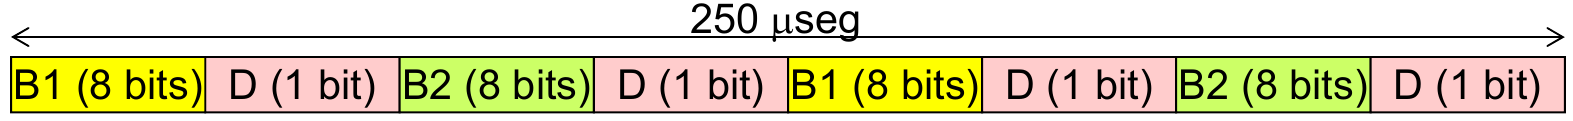
\includegraphics[
						width=10cm,
						%height=15cm
					]{Imágenes/Tema 3/Frame in S interface at basic rate.png}
					\caption{
						\label{fig:unit3_frame_S_basic}
						Frame in S interface at basic rate
					}
				\end{figure}
			}
			\item {
				Line coding:
				\begin{itemize}
					\item {
						Alternate Mark Inversion (AMI) is used:
						\begin{itemize}
							\item 0 $\rightarrow$ No signal.
							\item 1 $\rightarrow$ RZ bipolar pulses alternating the sign.
						\end{itemize}
					}
					\item {
						Frame alignment is obtained by violating the 1s signs' alternation.

						\begin{figure}[H]
							\centering
							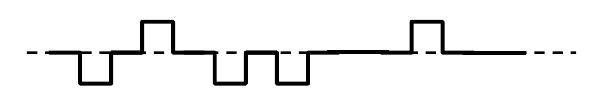
\includegraphics[
								width=10cm,
								%height=15cm
							]{Imágenes/Tema 3/Line coding in interface S at basic rate.png}
							\caption{
								\label{fig:unit3_coding_S_basic}
								Line coding in interface S at basic rate (1s signs' alternation)
							}
						\end{figure}
					}
					\item {
						The NT power supplies the terminal:
						\begin{itemize}
							\item Superimposing the DC signal into the signal or in a different pair.
							\item In a power failure, it gets the 48 V from the local exchange and it can power only one terminal (telephone).
						\end{itemize}
					}
				\end{itemize}
			}
		\end{itemize}
	}
	\item {
		At U interface:
		\begin{itemize}
			\item The data rate is 160 kbps.
			\item {
				Frame:
				\begin{itemize}
					\item {
						Each frame (240 bits) has 12 sets of 2B+D (18 bits) jointly with maintenance (6 bits) and synchronism (18 bits).

						\begin{figure}[H]
							\centering
							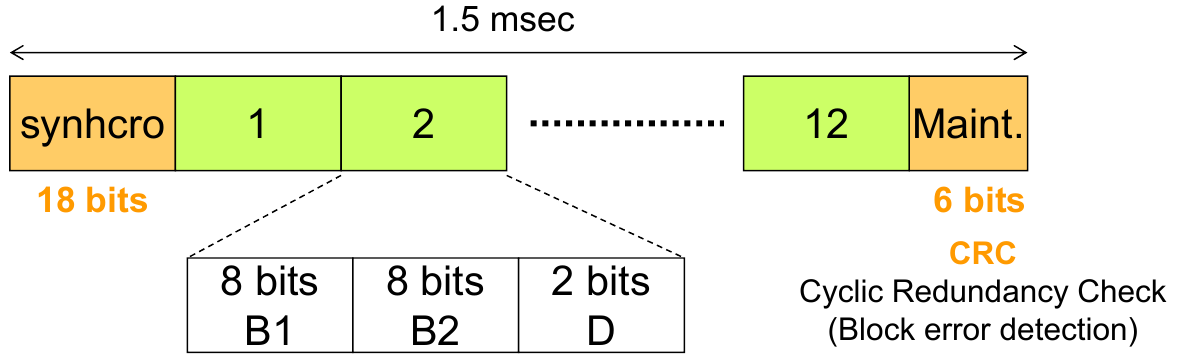
\includegraphics[
								width=12cm,
								%height=15cm
							]{Imágenes/Tema 3/Frame in U interface at basic rate.png}
							\caption{
								\label{fig:unit3_frame_U_basic}
								Frame in U interface at basic rate
							}
						\end{figure}
					}
					\item $80000 [pulses/sec]$ are sent in 2B1Q ($240[b]/1.5[ms] = 160 [kbps]$).
					\item {
						Synchronism slot rate:

						$
							\frac {1 \cdot 18 [b]} {1.5 \cdot 10^{-3} [s]} = 12 \cdot 10^3 [bps]
						$
					}
					\item {
						Maintenance slot rate:

						$
							\frac {6 [b]} {1.5 \cdot 10^{-3} [s]} = 4 \cdot 10^3 [bps]
						$
					}
					\item {
						One single channel B group rate:

						$
							\frac {12 \cdot 8 [b]} {1.5 \cdot 10^{-3} [s]} = 64 \cdot 10^3 [bps]
						$
					}
					\item {
						B channel rate:

						$
							\frac {12 \cdot 2 \cdot 8 [b]} {1.5 \cdot 10^{-3} [s]} = 128 \cdot 10^3 [bps]
						$
					}
					\item {
						D channel rate:

						$
							\frac {12 \cdot 2 [b]} {1.5 \cdot 10^{-3} [s]} = 16 \cdot 10^3 [bps]
						$
					}
					\item {
						Total channels rate:

						$
							\frac {12 \cdot 2 \cdot 8 [b] + 12 \cdot 2 [b]} {1.5 \cdot 10^{-3} [s]} = 144 \cdot 10^3 [bps]
						$
					}
					\item {
						Total rate:

						$
							\frac {1 \cdot 18 [b] + 1 \cdot 6 [b] + 12 \cdot 2 \cdot 8 [b] + 12 \cdot 2 [b]} {1.5 \cdot 10^{-3} [s]} = 160 \cdot 10^3 [bps]
						$
					}
				\end{itemize}
			}
			\item {
				Line coding for reducing the symbol rate:
				\begin{itemize}
					\item {
						2B1Q (ANSI standard and the trend is to keep it alone). Two bits are transmitted by a quaternary pulse ($-3$, $-1$, $+1$, $+3$).

						\begin{figure}[H]
							\centering
							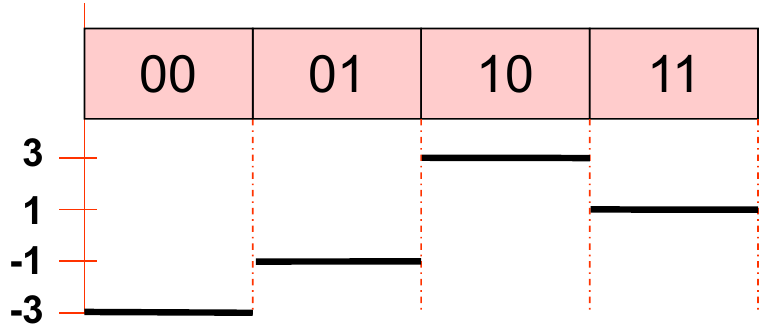
\includegraphics[
								width=6cm,
								%height=15cm
							]{Imágenes/Tema 3/2B1Q.png}
							\caption{
								\label{fig:unit3_2B1Q}
								2B1Q coding
							}
						\end{figure}
					}
					\item 4B3T
				\end{itemize}
			}
		\end{itemize}
	}
\end{itemize}

\subsubsection{Primary rate}

The useful data rate is calcluated in the following way for Europe:

$$
	30B + D = 30 \times 64 [kbps] + 64 [kbps] = 1984 [kbps]
$$

And for USA:

$$
	23B + D = 23 \times 64 [kbps] + 64 [kbps] = 1536 [kbps]
$$

Global data rate, including synchronism method, is 2048 kbps (PCM). Its applications are those that require both low capacity and high capacity user exchanges. Other configurations can be supported ($5H0 + D$, $H12 + D$, $31B$). It always work at 4W. It works in U interface:

\begin{itemize}
	\item {
		Line coding:
		\begin{itemize}
			\item The code method is High Density Bipolar Code (HDB3). It is similar to AMI, but limiting the transmission of many zeros in a row.
			\item In HDB3, any instance of four consecutive 0 bits is replaced with one of the patterns $000V$ (odd) or $B00V$ (even). The choice is made to ensure that consecutive violations are of differing polarity, this is, separated by an odd number of normal + or - marks.
			\item {
				To determine which pattern to use, one must count the number of pluses ($+$) and the number of minuses ($-$) since the last violation bit V:
				\begin{itemize}
					\item If the result is an odd number then $000-$ or $000+$ ($000V$) is used.
					\item If the result is an even number then $+00+$ or $-00-$ ($B00V$) is used.
				\end{itemize}
			}
			\item {
				To determine which polarity to use, one must look at the pulse preceding the four zeros:
				\begin{itemize}
					\item If odd ($000V$) form must be used, then $V$ simply copies the polarity of last pulse.
					\item If even ($B00V$) form must be used, then $B$ and $V$ chosen will have the opposite polarity of the last pulse.
				\end{itemize}
			}
		\end{itemize}
		\begin{table}
			\centering
			\begin{tabular}{|l|c|c|c|}
				\hline
				Parity of $+/-$ bits since previous $V$	& Pattern					& Previous pulse	& Code \\
				\hline
				\multirow{2}{*}{Even}					& \multirow{2}{*}{$B00V$}	& $+$				& $-00-$ \\
				\cline{3-4}
														&							& $-$				& $+00+$ \\
				\hline
				\multirow{2}{*}{Odd}					& \multirow{2}{*}{$000V$}	& $+$				& $000+$ \\
				\cline{3-4}
														&							& $-$				& $000-$ \\
				\hline
			\end{tabular}
			\caption{
				\label{tab:HDB3}
				High Density Bipolar Code (HDB3)
			}
		\end{table}
	}
	\item {
		Frame in Europe:

		\begin{itemize}
			\item {
				256 bits ($L = 256 [b/frame]$) in 125 microseconds ($T_{tx} = 125 [\mu s]$), 8000 frames per second ($f_{tx} = 1/T_{tx} = 8000 [frames/s]$), resulting in a 2048 kbps data rate ($C = f_{tx} \cdot L = 2048 [kbps]$).

				\begin{figure}[H]
					\centering
					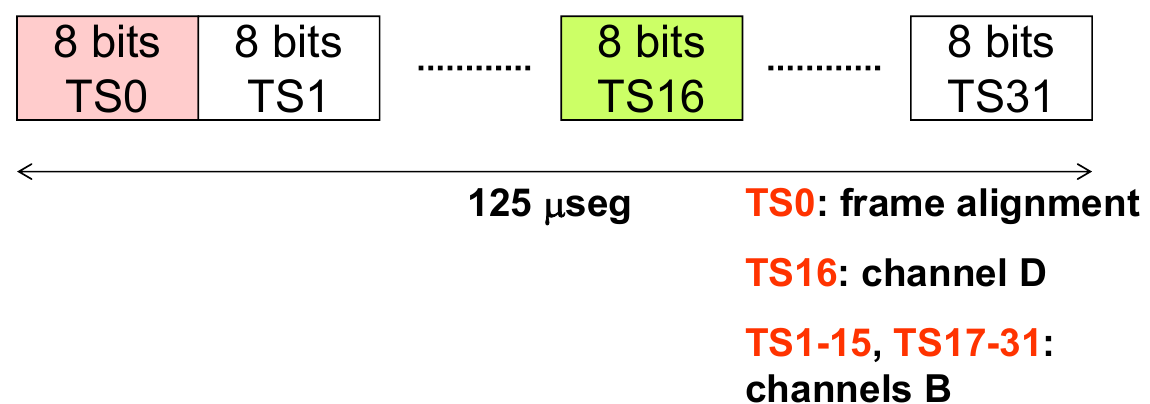
\includegraphics[
						width=9cm,
						%height=15cm
					]{Imágenes/Tema 3/Frame in U interface at primary rate (Europe).png}
					\caption{
						\label{fig:unit3_frame_U_primary_EU}
						Frame in U interface at primary rate (Europe)
					}
				\end{figure}
			}
			\item {
				Alignment slot rate:

				$
					\frac {1 \cdot 8 [b]} {125 \cdot 10^{-6} [s]} = 64 \cdot 10^3 [bps]
				$
			}
			\item {
				One single B channel slot rate:

				$
					\frac {1 \cdot 8 [b]} {125 \cdot 10^{-6} [s]} = 64 \cdot 10^3 [bps]
				$
			}
			\item {
				B channel rate:

				$
					\frac {30 \cdot 8 [b]} {125 \cdot 10^{-6} [s]} = 1920 \cdot 10^3 [bps]
				$
			}
			\item {
				D channel rate:

				$
					\frac {1 \cdot 8 [b]} {125 \cdot 10^{-6} [s]} = 64 \cdot 10^3 [bps]
				$
			}
			\item {
				Total channels rate:

				$
					\frac {30 \cdot 8 [b] + 1 \cdot 8 [b]} {125 \cdot 10^{-6} [s]} = 1984 \cdot 10^3 [bps]
				$
			}
			\item {
				Total rate:

				$
					\frac {1 \cdot 8 [b] + 30 \cdot 8 [b] + 1 \cdot 8 [b]} {125 \cdot 10^{-6} [s]} = 2048 \cdot 10^3 [bps]
				$
			}
		\end{itemize}
	}
	\item {
		Frame in USA:

		\begin{itemize}
			\item {
				193 bits ($L = 193 [b/frame]$) in 125 microseconds ($T_{tx} = 125 [\mu s]$), 8000 frames per second ($f_{tx} = 1/T_{tx} = 8000 [frames/s]$), resulting in a 1544 kbps data rate ($C = f_{tx} \cdot L = 1544 [kbps]$).

				\begin{figure}[H]
					\centering
					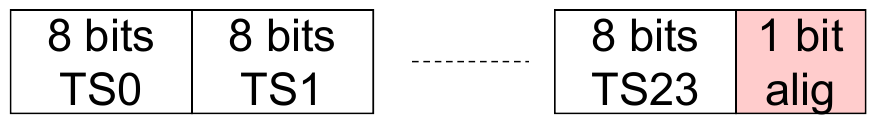
\includegraphics[
						width=7cm,
						%height=15cm
					]{Imágenes/Tema 3/Frame in U interface at primary rate (USA).png}
					\caption{
						\label{fig:unit3_frame_U_primary_USA}
						Frame in U interface at primary rate (USA)
					}
				\end{figure}
			}
			\item {
				Alignment slot rate:

				$
					\frac {1 \cdot 1 [b]} {125 \cdot 10^{-6} [s]} = 8 \cdot 10^3 [bps]
				$
			}
			\item {
				One single B channel slot rate:

				$
					\frac {1 \cdot 8 [b]} {125 \cdot 10^{-6} [s]} = 64 \cdot 10^3 [bps]
				$
			}
			\item {
				B channel rate:

				$
					\frac {23 \cdot 8 [b]} {125 \cdot 10^{-6} [s]} = 1472 \cdot 10^3 [bps]
				$
			}
			\item {
				D channel rate:

				$
					\frac {1 \cdot 8 [b]} {125 \cdot 10^{-6} [s]} = 64 \cdot 10^3 [bps]
				$
			}
			\item {
				Total channels rate:

				$
					\frac {23 \cdot 8 [b] + 1 \cdot 8 [b]} {125 \cdot 10^{-6} [s]} = 1536 \cdot 10^3 [bps]
				$
			}
			\item {
				Total rate:

				$
					\frac {23 \cdot 8 [b] + 1 \cdot 8 [b] + 1 \cdot 1 [b]} {125 \cdot 10^{-6} [s]} = 1544 \cdot 10^3 [bps]
				$
			}
		\end{itemize}
	}
\end{itemize}

\section{Digital Subscriber Loop (xDSL)}

\subsection{Introduction}

Copper subscriber loops are highly deployed. They have been used to increased data rate transmission, first, with modems, up to 56 kbps, later, on ISDN, up to 128 kbps. There are new technologies for increasing data rate over Mbps, all of them named Digital Subscriber Loop (xDSL):

\begin{itemize}
	\item High data rate DSL (HDSL): 2 Mbps duplex.
	\item Asymmetric DSL (ADSL): 1-8 Mbps DS or 16-640 Kbps US.
	\item Very high data rate DSL (VDSL): 13-52 Mbps DS or 1.5-2.3 Mbps US.
\end{itemize}

There are several systems for each technology: ADSL, ADSL2, ADSL2+, VDSL, VDSL2,... Mainly multi-carrier modulation. Echoe’s cancellation might be needed.

\subsection{Asymmetric DSL (ADSL)}

Different data rates for different directions (User $\leftrightarrow$ Network). Thus, different modems: ATU-R and ATU-C. There is a splitter system, two filters separate telephony from ADSL.

\begin{figure}[H]
	\centering
	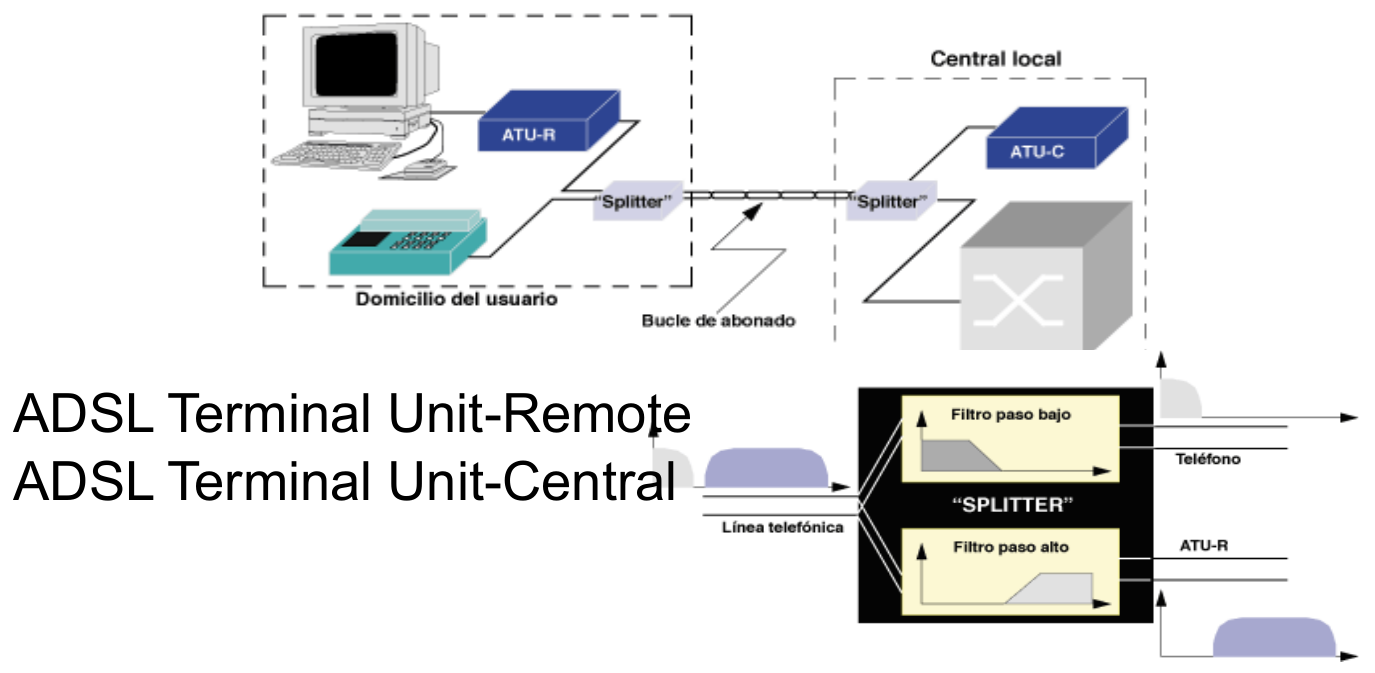
\includegraphics[
		width=14cm,
		%height=15cm
	]{Imágenes/Tema 3/ADSL.png}
	\caption{
		\label{fig:unit3_ADSL_scheme}
		ADSL scheme
	}
\end{figure}

It uses DMT modulation:

\begin{itemize}
	\item {
		Spectrum:

		\begin{figure}[H]
			\centering
			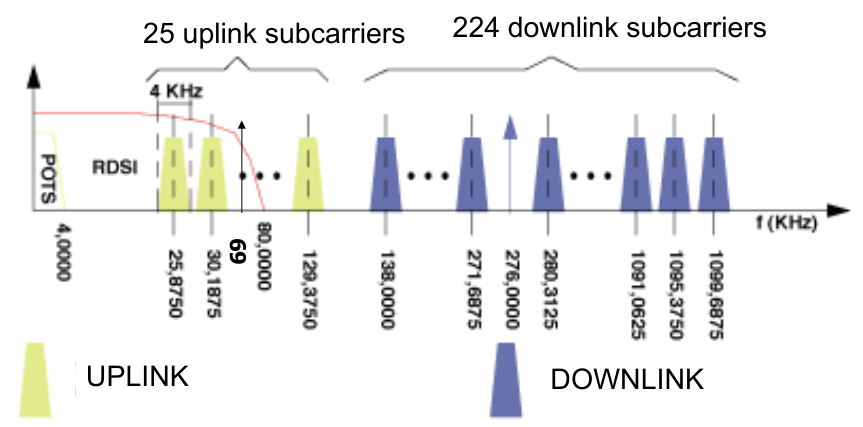
\includegraphics[
				width=10cm,
				%height=15cm
			]{Imágenes/Tema 3/ADSL spectrum.png}
			\caption{
				\label{fig:unit3_ADSL_spectrum}
				ADSL spectrum
			}
		\end{figure}
	}
	\item {
		Echo cancellation:

		\begin{figure}[H]
			\centering
			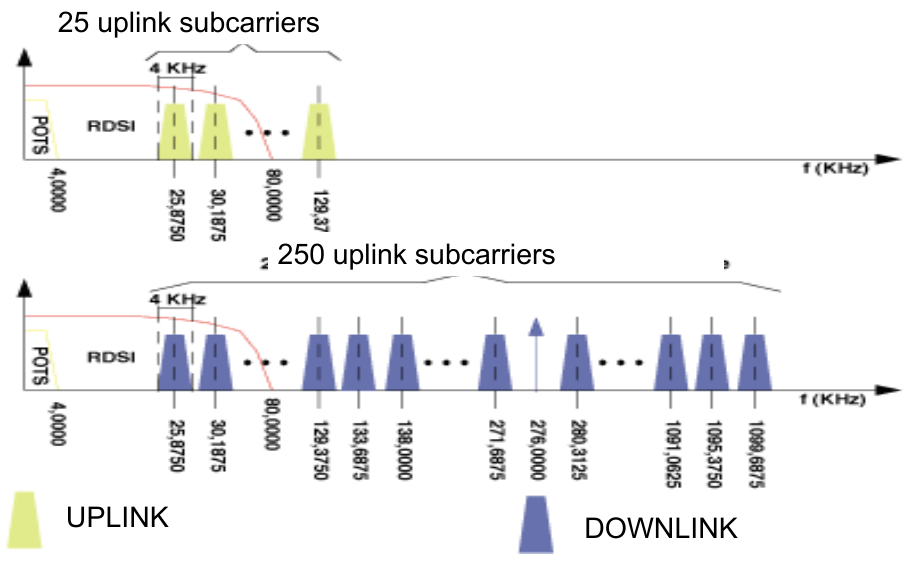
\includegraphics[
				width=10cm,
				%height=15cm
			]{Imágenes/Tema 3/ADSL echo cancellation.png}
			\caption{
				\label{fig:unit3_ADSL_echo}
				ADSL echo cancellation
			}
		\end{figure}
	}
\end{itemize}

Here is a comparison:

\begin{figure}[H]
	\centering
	\includegraphics[
		width=12cm,
		%height=15cm
	]{Imágenes/Tema 3/ADSL comparison.png}
	\caption{
		\label{fig:unit3_ADSL_comparison}
		ADSL comparison
	}
\end{figure}

\section{Synchronous Digital Hierarchy (SDH)}

\subsection{Introduction}

The SDH is a hierarchical set of digital transport structures, standardized for the transport of suitably adapted payloads over physical transmission networks. ITU-T provides with a set of recommendations: G.707, G.772, G.774.x, G.780, G.783, G.784, G.803, G.810, G.811, G.813, G.825, ...

The initial objectives were modest, such as the connection of different manufactures’ optical equipments (transversal compatibility). It is indeed a multiplexing technique the one that allows the transportation of ``payloads'' from digital hierarchies (1.5 Mbps in USA and Japan, 2 Mbps at international level). Motivations behind SDH include:

\begin{itemize}
	\item High speed optical elements.
	\item Reduction in wires.
	\item Remote managements of equipments and circuits.
	\item Transversal compatibility.
	\item Broadband and narrowband compatibility.
\end{itemize}

\subsection{Synchronous Transfer Module (STM-N)}

SDH defines a format for transfer among network called Synchronous Transfer Module (STM), which is defined for different levels (N).

\subsubsection{Levels}

\begin{tabular}{|c|c|c|c|}
	\hline
	STM-N	& Digital hierarchy	& Rate (Mbps)	& Electrical/Optical interface \\
	\hline
	SMT-1	& Level 1			& 155,520		& G.703/G.957 \\
	\hline
	STM-4	& Level 4			& 622,020		& ---/G.957 \\
	\hline
	STM-16	& Level 16			& 2488,320		& ---/G.957 \\
	\hline
	STM-64	& Level 64			& 9953,280		& ---/G.957 \\
	\hline
	STM-256	& Level 256			& 9953,280		& ---/G.957 \\
	\hline
\end{tabular}

\subsubsection{STM-1 frame structure}

STM-1 frame structure can be described with the following points:

\begin{itemize}
	\item $9 [rows] \times 270 [columns]$
	\item Each cell is an octet (a byte $B$).
	\item Capacity: $9 \times 270 [B] = 2430 [B] = 19440 [b]$
	\item Frame length: $125 [\mu s] \rightarrow T_{tx} = 125 [\mu s]$
	\item Section OverHead: $SOH = RSOH (3 \times 8 [B] = 24 [B]) + MSOH (5 \times 8 [B] = 40 [B]) = 64 [B]$
	\item Pointer: $1 \times 8 [B] = 8 [B]$
	\item Payload: $9 \times 262 [B] = 2358 [B]$
	\item $R_b = 8000 [frame/s] \cdot 2430 [B/frame] \cdot 8 [b/B] = 155520000 [bps]$
\end{itemize}

\begin{figure}[H]
	\centering
	\includegraphics[
		width=10cm,
		%height=15cm
	]{Imágenes/Tema 3/STM-1 frame.png}
	\caption{
		\label{fig:unit3_STM1_frame}
		STM-1 frame
	}
\end{figure}

\subsubsection{Inserting C4 into STM-1}

To manage payload, a virtual container must be inserted:

\begin{itemize}
	\item C-x (Container): Spatial division (time too) for the payload.
	\item VC-x (Virtual Container)
	\item AU-x (Administrative Unit): spatial division for the frame into the line
	\item AU-PTR: pointer, indicates the starting point of a VC-x within the STM-1
\end{itemize}

\begin{figure}[H]
	\centering
	\includegraphics[
		width=10cm,
		%height=15cm
	]{Imágenes/Tema 3/STM-1 frame with C4.png}
	\caption{
		\label{fig:unit3_STM1_C4}
		STM-1 frame with C4
	}
\end{figure}

\subsection{Multiplex}

\begin{figure}[H]
	\centering
	\includegraphics[
		width=12cm,
		%height=15cm
	]{Imágenes/Tema 3/SDH multiplex.png}
	\caption{
		\label{fig:unit3_STM1_multiplex}
		SDH multiplex
	}
\end{figure}

\subsection{Equipment}

Equipment includes:

\begin{itemize}
	\item {
		Regenerator

		\begin{figure}[H]
			\centering
			\includegraphics[
				width=7cm,
				%height=15cm
			]{Imágenes/Tema 3/Regenerator.png}
			\caption{
				\label{fig:unit3_regenerator}
				SDH regenerator
			}
		\end{figure}
	}
	\item {
		Terminal multiplexer (TM)

		\begin{figure}[H]
			\centering
			\includegraphics[
				width=5cm,
				%height=15cm
			]{Imágenes/Tema 3/TM.png}
			\caption{
				\label{fig:unit3_TM}
				SDH terminal multiplexer (TM)
			}
		\end{figure}
	}
	\item {
		Add and drop multiplexer (ADM)

		\begin{figure}[H]
			\centering
			\includegraphics[
				width=4cm,
				%height=15cm
			]{Imágenes/Tema 3/ADM.png}
			\caption{
				\label{fig:unit3_ADM}
				SDH add and drop multiplexer (ADM)
			}
		\end{figure}
	}
	\item {
		Digital cross-connect (DXC)

		\begin{figure}[H]
			\centering
			\includegraphics[
				width=4cm,
				%height=15cm
			]{Imágenes/Tema 3/DXC.png}
			\caption{
				\label{fig:unit3_DXC}
				SDH digital cross-connect (DXC)
			}
		\end{figure}
	}
\end{itemize}

\subsection{SubNetwork Connection Protection (SNCP)}

SNCP transmits by both directions in the ring.

\begin{figure}[H]
	\centering
	\includegraphics[
		width=5cm,
		%height=15cm
	]{Imágenes/Tema 3/SNCP.png}
	\caption{
		\label{fig:unit3_SNCP}
		SDH SubNetwork Connection Protection (SNCP)
	}
\end{figure}

\subsection{Multiplex Section - Shared Protection Rings (MS-SPRing)}

Only valid for STM-16 and above. The protection capacity is shared in all the ring. If it is not needed, it can be used for extra traffic.

\begin{figure}[H]
	\centering
	\includegraphics[
		width=14cm,
		%height=15cm
	]{Imágenes/Tema 3/MS-SPRing.png}
	\caption{
		\label{fig:unit3_MS_SPRing}
		SDH Multiplex Section - Shared Protection Rings (MS-SPRing)
	}
\end{figure}

\section{(Dense) Wavelength Division Multiplexing ((D)WDM)}

\subsection{Introduction}

The all-optical networks are very young (since 2000):

\begin{itemize}
	\item {
		Until 2000, almost optical networks:
		\begin{itemize}
			\item Only fiber.
			\item One wavelength, usually 1310 nm (optimized) in singlemode fibers.
			\item Optical-electrical interfaces are inefficient.
		\end{itemize}
	}
	\item In 80, 50 Mbps (ODL-50 devices).
	\item Proprietary designs appeared. All disappeared with SONET/SDH.
	\item Limit per fiber is 40 Gbps (10 Gbps in 90’s).
	\item In 90’s, large bandwidth demands. Several fibers are put together.
\end{itemize}

New technologies such as WDM (Wavelength Division Multiplexing) and Dense WDM came up:

\begin{itemize}
	\item A single fiber carries several wavelengths. Example: 40 wavelengths per fiber, each with 40 Gbps gives 1.6 Tbps per fiber.
	\item Between 8 - 32 wavelengths: Coarse WDM
	\item More than 40: DWDM
\end{itemize}

\begin{figure}[H]
	\centering
	\includegraphics[
		width=12cm,
		%height=15cm
	]{Imágenes/Tema 3/(D)WDM.png}
	\caption{
		\label{fig:unit3_DWDM}
		(D)WDM sheme
	}
\end{figure}

It is highly likely that in near future we will have FttPC (Fiber to the PC).

Advantages:

\begin{itemize}
	\item Large capacity per fiber
	\item {
		Scales easily:
		\begin{itemize}
			\item No new fibers are needed, only add new wavelengths.
			\item Incremental cost per extra channel is low.
			\item No too much changes in the hardware.
		\end{itemize}
	}
	\item The fiber span is much larger with DWDM than TDM (SONET/SDH). Chromatic dispersion and polarization in TDM
\end{itemize}

Disadvantages:

\begin{itemize}
	\item Very expensive for few channels. Fixed costs such as the mux/demux, transponders and other components.
	\item Introduces a new parameter in the design and management: the wavelength.
	\item SONET/SDH networks are not well prepared for DWDM.
	\item Monitoring DWDM signals still needs research.
\end{itemize}

\subsection{CWDM Advantages}

CWDM is cheaper than DWDM, about 30\%. That’s because:

\begin{itemize}
	\item Cheaper lasers since less precision and control is required.
	\item Passive components such as multiplexers can be obtained at low cost.
	\item CWDM components need less physical space in PCBs, which implieas a lower cost.
\end{itemize}

\subsection{SXG-PON}

PON (Pasive Optical Network). Provide FTTH services.

\begin{tabular}{|l|l|l|l|l|}
	\hline
						& G-PON	& XG-PON	& SXG-PON	& NG-PON \\
	\hline
	Upstream (Gbps)		& 1,5	& 2,5		& 10		& 40 \\
	\hline
	Downstream (Gbps)	& 2,5	& 10		& 10		& 40 \\
	\hline
						& Gigabit			& 10 Gbit	& Symmetric XG	& Next generation \\
	\hline
\end{tabular}

\subsection{Applications}

Main applications:

\begin{itemize}
	\item Metropolitan Area Networks. Up to FttPC.
	\item CATV
\end{itemize}

Supports:

\begin{itemize}
	\item IP
	\item SDH/SONET
	\item ATM
	\item Frame-Relay
	\item Ethernet
	\item Multi-protocol Label System (MPLS) and its adaptation M$\lambda$LS.
\end{itemize}

\chapter{Terrestrial mobile communications systems}

\section{PMR and PMT systems}

\subsection{Introduction}

PMR and PMT systems

\subsection{Private Mobile Radio (PMR)}

Usually not directly connected to public telephony network. Modeled as waiting systems. The PMR main characteristics are:

\begin{itemize}
	\item Limited Area (territorial).
	\item No usually directly connected to public switching telephony networks (PSTN)
	\item Fleet management. Enterprises.
	\item Example: TETRA (Trans European Trunked Radio)
\end{itemize}

Other characteristics:

\begin{itemize}
	\item MS to MS calls must be allowed.
	\item Calls are frequent and short in duration.
	\item Group calls must be permitted.
	\item Work in waiting regime, this is, they are modeled as waiting systems.
	\item Usually simplex (one or two frequencies) or semiduplex PTT (push to talk), although they can also be duplex.
\end{itemize}

Channel assignment:

\begin{itemize}
	\item Fixed Assignment: the channel is fixed for a group of M users that need to share it. It is simpler but lower performance. Used if the number of users is low.
	\item Trunked Assignment: pool of N channels being shared for M users. More complex but much more efficient.
\end{itemize}

Trunking Systems:

\begin{itemize}
	\item Pool of channels where the channel assignment is dynamic.
	\item They are waiting as the fixed assignment.
	\item A signaling protocol is needed for channel assignment and managing calling queues.
	\item In Europe, MPT 1327 protocol was developed in UK, which has been converted in fact the standard for such as systems. It is based on slotted ALOHA with variable frame length.
\end{itemize}

\subsection{Personal Mobile Telecommunications (PMT)}

Connected directly to public Telephony Network. Modeled as blocking systems. It is the public radio-telephony service, so it offers the mobile telephony service to the users. Any user, from a parked or moving vehicle, can sends or receive calls of/to any other fixed or mobile subscriber either national or international. These systems are, indeed, the PLMN (Public Land Mobile Network) with its own switching centers MSC (Mobile Switching Centers), that are connected to the public switched telephony service or other networks such as ISDN, data networks,

....

The main objectives are:
\begin{itemize}
	\item Large subscribers capacity to attend high traffic demands.
	\item Voice quality equal or higher than fixed service.
	\item Spectrum efficiency since we manage a limited number of frequencies, so frequency usage must be planned. The solution is frequency reuse by cellular planning.
	\item Radio frequency automatic switching.
	\item Capacity of expansion to achieve large coverage.
	\item Reasonable costs
\end{itemize}

Related concepts:
\begin{itemize}
	\item Handoff or handover: BS switching of a current voice call.
	\item Roaming: The mobile terminal moves from the own network to a different one.
	\item Downlink or direct channel: Radio channel for transmission from BS to MS (BS$\rightarrow$MS).
	\item Uplink or return channel: Radio channel for transmission from MS to BS (MS$\rightarrow$BS). Lower frequencies in the band are allocated to it.
\end{itemize}

\section{Trunking systems: TETRA}

\subsection{Introduction}

The trunking systems are private radio telephony services offered to a closed group of users (usually a vehicle fleet, like police, firemans, ambulances, public transportation, ...), which are locally or even regionally located. The trunking network is shared among several groups by using dynamic radio channel allocation. When one user requests a call to another user, the system allocates a free radio channel from the pool and, once the call is finished, it is released.

The main difference with respect to Automatic Mobile Telephony like GSM is the way the call is processed. The trunking system is the one who handles calls by establishing a queue for all the incoming pending calls. Then, according to the arrived order or the priority, the call is sent. On the other hand, in PMT systems, the user is the one who needs to call again if the call is blocked in the system. It is a waiting system instead of a blocking one. The management of a trunking system aims to get a very efficient use of resources, even obtaining a higher efficiency than traditional systems. The trunking system is able to use the pauses in normal voice transmission to give access to other calls.

\subsection{Terrestrial Trunking Radio (TETRA)}

It is the 2nd generation of standards for PMR systems in Europe. Among the facilities of TETRA we
have:

\begin{itemize}
	\item Duplex voice and data transmission.
	\item Data transmission up to 28.8 kbps.
	\item Optimized packet data transmission.
	\item Telemetry and slow video transmission.
	\item Communications security.
	\item Wide number of interfaces for interconnection with other networks.
	\item {
		Two modes:
		\begin{itemize}
			\item Voice + Data mode (V+D): Normal mode for telephony applications and data.
			\item Packet Data Optimized (PDO): It allows new data services such as e-mail, data interchange, location, ...
		\end{itemize}
	}
\end{itemize}

About radio interface:

\begin{itemize}
	\item {
		Basic radio interface specifications:
		\begin{itemize}
			\item 25 kHz channelization (optional 12.5 kHz).
			\item TDMA multiple-access with four intervals per frame.
			\item $\pi/4$ - DPSK modulation.
			\item Data rate 36 kbps.
			\item Protection rate of 19 dB.
		\end{itemize}
	}
	\item Within TDMA hierarchy. It uses a slot of 85/6 ms duration with capacity of 510 bits.
	\item Frame composed by four slot. Its duration is 56.67 ms.
	\item Multiframe composed by 18 frames. Its duration is 1.020 ms.
	\item Hiperframe composed by 60 multiframes.
\end{itemize}

\begin{tabular}{|c|c|c|c|c|}
	\hline
	Ramp	& Data		& Training		& Data		& Ramp \\
	\hline
	13 bits	& 216 bits	& 14+22+16 bits	& 216 bits	& 13 bits \\
	\hline
\end{tabular}

\section{Cellular systems}

\subsection{Introduction}

The covered area is divided in smaller ones denoted cells. The co-channel distance or reuse distance is the distance between two cells using the same frequencies with respect to the protection rate. These radio systems are limited by interference. All the frequencies are assigned to a group of cells denoted as cluster. The area is covered by the cluster (GSM).

\begin{figure}[H]
	\centering
	\includegraphics[
		width=10cm,
		%height=15cm
	]{Imágenes/Tema 4/Cellular systems description.png}
	\caption{
		\label{fig:unit4_cells_scheme}
		Cellular system scheme
	}
\end{figure}

In the figure \ref{fig:unit4_cells_scheme}, the area is covered by clusters reusing the same frequencies. D is the co-channel distance. We can develope the following relations:

\begin{itemize}
	\item {
		Basic propagation losses:

		$I_b = k \cdot r^n$
	}
	\item {
		$c = \frac {P_t} {k \cdot R^n}$
	}
	\item {
		$i = \frac {P_t} {k (D - R)^n}$
	}
	\item {
		$
			\left.
				\begin{matrix}
					c = \frac {P_t} {k \cdot R^n} \\
					i = \frac {P_t} {k (D - R)^n}
				\end{matrix}
			\right\rbrace \rightarrow
			\frac {c} {i} = \left( \frac {D - R} {R} \right)^n \approxeq \left( \frac {D} {R} \right)^n
		$
	}
\end{itemize}

If $R$ and $D$ are decreased, holding a given $\frac {c} {i}$, we can increase the reuse of frequencies and system capacity. However, $R$ is lower bounded by the protection rate:

$$\left( \frac {c} {i} \right)_{MIN} = r_p$$

\subsection{Dimensioning}

Mobile cellular systems are designed as blocking systems:

$$
	p = B(N, A)
$$

Where:
\begin{itemize}
	\item $p$: Blocking probability.
	\item $N$: Available number of radiofrequency channels in the cell.
	\item $A$: Offered traffic.
\end{itemize}

For the number of available channels:

$$
	C = \frac {W} {\Delta f} = \frac {W} {f_2 -  f_1}
$$

Where:
\begin{itemize}
	\item $W$: Available bandwidth for transmission or reception.
	\item $\Delta f$: Separation between radio frequency channels.
\end{itemize}

If the cluster has $J$ cells, the number of radiofrequency channels in a cell is:

$$
	N = \frac {C} {J}
$$

Assuming that the median call duration is $H$ seconds and the mean number of calls at Busy Hour is $L$, the offered traffic per user will be:

$$
	a = H \cdot \frac {L} {3600} [E]
$$

The offered traffic in a cell is:

$$
	A = B^{-1} (N - 1, p)
$$

Where $B^{-1}$ stands for Erlang B inverse function, and $p$ is the blocking probability. Usually, $N - 1$ radio frequency channels are considered because one is reserved for signaling purposes.

The number of mobile users in a cell is:

$$
	m = \frac {A} {a}
$$

The allowable traffic intensity in the cell is:

$$
	\rho_a = \frac {A} {S_c} [E / km^2]
$$

Where $S_c$ is the cell area in km$^2$.

Then, the area for the cluster is:

$$
	S_r = J \cdot S_c
$$

If the coverage area must be $S$, the number of clusters will be:

$$
	Q = integer \left( \frac {S} {S_r} \right) + 1 \approxeq \frac {S} {J \cdot S_c}
$$

$Q$ is also the number of times that frequencies are reused and it is considered the reuse factor.

The whole number of channels for traffic in the coverage area will be:

$$
	Q \cdot J \cdot (N - 1) \approxeq C \cdot \frac {S} {J \cdot S_c}
$$

And the total number of users will be:

$$
	M = Q \cdot J \cdot m
$$

\subsection{Cellular geometry}

If in a cell, omnidirectional antennas are used, the coverage area will be approximately circular, but circles do not cover the whole plane without overlapping. Other polygons are used to cover the plane without overlapes, there are three regular ones: triangle, square and hexagon. The one with largest ratio area/radio is the hexagon, and so, it is used.

An inclined coordinated systems is used with a slope of 60º.

\begin{figure}[H]
	\centering
	\includegraphics[
		width=10cm,
		%height=15cm
	]{Imágenes/Tema 4/Cellular geometry.png}
	\caption{
		\label{fig:unit4_cell_geometry}
		Cellular geometry
	}
\end{figure}

The parameters to study cellular geometry are:
\begin{itemize}
	\item $D$: Co-channel distance. One of them is located in the origin of coordinates.
	\item $d$: Lattice step.
	\item $i_c$, $j_c$: co-channel node coordinates.
	\item $J$: The numbers obtained given integer values to $i_c$ and $j_c$ are known as rhombic numbers (1, 3, 4, 7, 9, 12, 13, 16, 19, 21, 25, 27, 28, 36, 37, 48, ...). $J$ also represents the cluster size, being each cell surrounded by 6 co-channel cells at distance $D$.
\end{itemize}

Relations are:
\begin{itemize}
	\item {
		Distance from origin to the co-channel cell:

		$D = \left( d(i, j) \right)^2 = d^2 (i^2 + j^2 + i \cdot j)$
	}
	\item $d = R \sqrt{3}$
	\item $\left( \frac {D} {d} \right)^2 = i_{c}^2 + j_{c}^2 + i_{c} \cdot j_{c} = J$
	\item $J = \frac {1} {3} \left( \frac {D} {R} \right)^2$
	\item {
		$J$ is lower bounded by protection rate:
		\begin{itemize}
			\item {
				Signal at the edge of the cell and interference at the center:

				$\left( \frac {c} {i} \right)_{TOT} = \frac {1} {6} \left( \frac {D} {R} \right)^n \rightarrow J = \frac {1} {3} \left[ 6 \left( \frac {c} {i} \right)_{TOT} \right]^{\frac {2} {n}}$

				$\left( \frac {c} {i} \right)_{TOT} \geq r_p \rightarrow J \geq \frac {1} {3} \left( 6 r_p \right)^{\frac{2}{n}}$
			}
			\item {
				Signal and interference at the edge:

				$\left( \frac {c} {i} \right)_{TOT} = \frac {1} {6} \left( \frac {D - R} {R} \right)^n \rightarrow J = \frac {1} {3} \left( 1 + \left[ 6 \left( \frac {c} {i} \right)_{TOT} \right]^{\frac {1} {n}} \right)^2$

				$\left( \frac {c} {i} \right)_{TOT} \geq r_p \rightarrow J \geq \frac {1} {3} \left[ 1 + \left( 6 r_p \right)^{\frac{1}{n}} \right]^2$
			}
		\end{itemize}
	}
\end{itemize}

\subsection{Cellular division}

Cells can be divided into smaller ones according to demand (rural areas, urban areas, dense urban areas, etc.). It gives more flexibility to the planning process. The evolution is progressive. Dividing by two comes with:

\begin{itemize}
	\item Reduction in radio of the cell in half.
	\item Reduction of cell area by four.
	\item Increase in capacity approximately in four.
	\item BTS location must be more precise.
	\item The probability of handover is increased.
	\item Costs are increased.
\end{itemize}

\subsection{Sectoring}

Instead of using omnidirectional antennas at the very centre of each cell, directive antennas at the cell edges are used. In this way, the number of interference sources can be reduced due to antenna directivity.

Sectoring is carried out dividing the original cell into sectors that are covered by base stations at the alternate hexagon’s vertex.

\begin{figure}[H]
	\centering
	\includegraphics[
		width=14cm,
		%height=15cm
	]{Imágenes/Tema 4/Cellular sectoring 1.png}
	\caption{
		\label{fig:unit4_cell_sect_1}
		Cellular sectoring
	}
\end{figure}

This structure has some advantages:

\begin{itemize}
	\item The BTS can be supported by adjacent BTS cells, so we save in infrastructures.
	\item The co-channel interference is much lower due to the directivity of antennas. Thus, J can be lower and then, the system capacity is higher due to the higher frequency reuse.
\end{itemize}

\begin{figure}[H]
	\centering
	\includegraphics[
		width=7.5cm,
		%height=15cm
	]{Imágenes/Tema 4/Cellular sectoring 2.png}
	\caption{
		\label{fig:unit4_cell_sect_2}
		Cellular sectoring
	}
\end{figure}

\section{Global System for Mobile Communications (GSM)}

\subsection{Introduction}

GSM is a mobile communications standard developed by ETSI. It is second generation communication system.

\subsection{Description}

\subsubsection{Services}

GSM attend a series of services:

\begin{itemize}
	\item {
		Basic Services:
		\begin{itemize}
			\item Bearer Services: Synchronous/Asynchronous transport capacity, packet or circuit mode at 9.600 bps.
			\item {
				Teleservices:
				\begin{itemize}
					\item Digital telephony with codec at total speed of 13 kbps or codec at half speed of 6.5 kbps.
					\item Short Messages Service (SMS).
					\item Facsimile: FAX Group 3.
				\end{itemize}
			}
		\end{itemize}
	}
	\item {
		Supplementary services:
		\begin{itemize}
			\item Calling line identification.
			\item Explicit call transfer.
			\item Waiting calls.
			\item Voice mail.
			\item Multi-party conferences.
			\item Billing (free calls, call collect, \ldots).
		\end{itemize}
	}
\end{itemize}

\subsubsection{Characteristics}

GSM main characteristics are:

\begin{itemize}
	\item It uses GMSK modulation.
	\item {
		Protection co-channel rate:

		$\frac {C} {I_c} = 9 [dB]$

		$\frac {S} {I} = 10 \cdot \log \left( \frac {\left( \sqrt{3 J} \right)^n} {i_0} \right)$
	}
	\item Channel bandwidth: 200 kHz 8 channels/carrier
	\item Doppler distortion: Up to 200 km/h can be compensated.
	\item Temporal distortion: Up to 16 $\mu$s can be equalized.
	\item Cellular structure: Sectored in urban areas and omnidirectional in rural areas.
	\item Multiple-Access: TDMA with 8 intervals per frame (8 physical channels per carrier frequency).
	\item Frequency Hopping (FH): Mobile Subscriber (MS) can change the frequency from frame to frame (217 hops per second) in order to avoid the multipath fading.
	\item Discontinuous Tx (DTX): Data is only sent when user is talking, otherwise, comfort noise is generated at receiver.
	\item Security: Communications are ciphered and access system authentication is required.
	\item {
		Frequency bands for GSM-900 in its P version (most extended one) are:
		\begin{itemize}
			\item MS-BS link: 890 - 915 MHz (25 MHz).
			\item BS-MS link: 935 - 960 MHz (25 MHz).
		\end{itemize}
		These bands are divided into 124 pairs separated 200 kHz each other:

		$f_{MS-BS} = 890.2 + 0.2 \cdot (n - 1) [MHz]$

		$f_{BS-MS} = f_{MS-BS} + 45 [MHz] = 935.2 + 0.2 \cdot (n - 1) [MHz]$

		$n = 0, 1, 2, \ldots, 125$
	}
	\item {
		Frequency bands for GSM-DCS-1800 are:
		\begin{itemize}
			\item Uplink: 1710 - 1785 MHz (75 MHz).
			\item Downlink: 1805 - 1880 MHz (75 MHz).
		\end{itemize}
	}
\end{itemize}

\subsubsection{Mobile Subscriber (MS) identification}

In order to identify and manage Mobile Subscribers (MS), GSM defines the following information fields:

\begin{itemize}
	\item International Mobile Equipment Identity (IMEI): It identifies the terminal and is burnt by manufacturer.
	\item International Mobile Subscriber Identity (IMSI): It identifies the user internationally. It is associated to SIM card. IMSI is not known by the user, except spoiler. It is used by the network for authentication and call establishment. It is used the first time (GSM attach) and then it is changed to a temporal one (TMSI), assigned by a device called VLR.
	\item Temporal Mobile Subscriber Identity (TMSI): Temporal mobile subscriber identity assigned by VLR.
	\item {
		Mobile Station ISDN (MS-ISDN): It is the user telephone number. It follows the format:

		\texttt{CC (country) | NDC (operator prefix) | Subscriber number}
	}
	\item Mobile Subscriber Roaming Number (MSRN): It is another number used for routing.
\end{itemize}

\subsection{Architecture}

\subsubsection{Elements}

GSM architecture is implemented through the following elements:

\begin{itemize}
	\item Public Switching Telephony Network (PSTN).
	\item Mobile Switching Center (MSC): It manages calls from or to MS and establishes conections with other networks (PSTN, ISDN, \ldots).
	\item Home Location Register (HLR): It is the whole subscriber register. It stores IMSI, MSISDN, location information, \ldots
	\item Visitors Location Register (VLR): It is the visiting subscribers register for temporal users controlled by the MSC. It stores IMSI, TMSI, MSRN and a copy of profile data from HLR for users.
	\item Base Station Controller (BSC): Most functions are at the BSC, allowing BTS being very simple.
	\item Base Transceiver Station (BTS).
	\item Mobile Terminal (MT).
	\item Terminal Equipment (TE).
	\item Authentication Center (AUC): It is the authentication center. It stores identity information for users to verify calls and users.
	\item Equipment Identity Register (EIR).
	\item Operation and Maintenance Center (OMC).
	\item Network Management Center (NMC).
	\item Administration Center (ADC).
	\item Operation Subsystem (OSS).
	\item Base Station Subsystem (BSS).
	\item Mobile Station (MS).
\end{itemize}

\subsubsection{Interfaces}

Two main interfaces have been defined:

\begin{itemize}
	\item Line interface (A): It separates the switching center (MSC) and the base station subsystem (BSS). There is also an optional interface (A-bis) between the BSC and BTS.
	\item Radio interface (Um): It places the borderline between base stations and mobile terminals (MS).
\end{itemize}

\subsubsection{Scheme}

\includegraphics[
	width=10cm,
	%height=15cm
]{Imágenes/Tema 4/GSM architecture.png}

\subsection{GSM frame}

\subsubsection{Frame structure}

Each GSM frame is composed by 8 time-slots. The frame duration is 4,615 ms and thus, each time-slot is lasts 0,577 ms. This structure is for uplink and downlink, but with a delay of 3 time-slots. In this way, a mobile transmits or receives, but not both simultaneously.

\begin{figure}[H]
	\centering
	\includegraphics[
		width=7cm,
		%height=15cm
	]{Imágenes/Tema 4/GSM frame.png}
	\caption{
		\label{fig:unit4_GSM_frame}
		GSM frame
	}
\end{figure}

\subsubsection{Burst}

Data information is sent inside the time-slot in a burst of bits. Each burst has 148 bits. At the end of the burst, the time equivalent of 8.25 bits is appended as guard period. Thus, the data rate at the radio interface is:

$$
	\frac {156.25 [b]} {0.577 [ms]} = 270.833 [kbps]
$$

There are several types of burst:
\begin{itemize}
	\item Normal burst.
	\item Frequency correction burst.
	\item Synchronization burst.
	\item Dummy burst.
	\item Access burst.
\end{itemize}

Normal burst has 148 bits and the guard period (156.25 bits in total):
\begin{itemize}
	\item Tail Bits (TB): 3+3 bits of header (one header for each data bits set).
	\item Data bits: 2 x (57 bits + 1 bit) = 116 bits. Two sets of data bits. The 57 bits part is information, and the other bit is a flag to indicate if is TCH or FACCH.
	\item Training Sequence (TS): 26 bits. Used for channel estimation and adjusting the equalizer.
	\item Guard Period (GP): Time equivalent to 8.25 bits.
\end{itemize}

\begin{tabular}{|c|c|c|c|c|c|}
	\hline
	TB 1 (3 bits)	& Data 1 (58 bits)	& TS (26 bits)	& Data 1 (58 bits)	& TB 2 (3 bits)	& GP (8.25 bits) \\
	\hline
\end{tabular}

\subsubsection{Hierarchy}

The frame hierarchy can be visualized in the following picture:

\includegraphics[
	width=12cm,
	%height=15cm
]{Imágenes/Tema 4/GSM frame hierarchy.png}

\subsection{Logical channels}

GSM establishes a set of logical channels.

\subsubsection{Traffic channels (TCH)}

They are mapped onto a pair of subcarriers and slots. There are seven types for these channels:
\begin{itemize}
	\item Full rate voice (TCH/F).
	\item Half rate voice (TCH/H).
	\item Data at speed of 2.4, 4.8 and 9.6 kbps.
	\item Data at half speed of 2.4 and 4.8 kbps.
\end{itemize}

In each communication, each traffic channel has a signaling channel associated to control the call:
\begin{itemize}
	\item Slow Associated Control Channel (SACCH): Common signaling associated to the voice call such as power control, billing, timing advanced, quality, \ldots
	\item Fast Associated Control Channel (FACCH): Urgent signaling such as in handovers. It steals bits to the traffic channel.
\end{itemize}

\subsubsection{Signaling channels}

\begin{itemize}
	\item {
		Broadcast channels: They work in the downlink and they are intended for all the terminals. They are supposed to help in synchronization, for example:
		\begin{itemize}
			\item Broadcast Control Channel (BCCH): General cell information and network.
			\item Frequency Correction Channel (FCCH): It is used for frequency acquisition by the MS.
			\item Synchronization Channel (SCH): It is used for synchronization and BS identification purposes.
		\end{itemize}
	}
	\item {
		Common control channels (CCCH): They are used to control the access to the network from terminals. They are uplink and downlink. They are:
		\begin{itemize}
			\item Ramdom Access Channel (RACH): Uplink. MSs request the access to the network (e.g., originated call). Slotted ALOHA is used.
			\item Paging Channel (PCH): Downlink. The network notifies to MS about incoming calls or messages.
			\item Access Grant Channel (AGCH): Downlink. Resource assignments.
		\end{itemize}
	}
	\item {
		Dedicated control channels: Bidirectional channels dedicated between a MS and the network. Previous to a call transmission:
		\begin{itemize}
			\item Stand-alone Dedicated Control Channel (SDCCH): Divided into 8 channels (D0, D1, \ldots, D7), each one is associated to one MS for signaling purposes.
			\item Slow Associated Control Channel (SACCH): It is the associated control channel for the SDCCH. It is also divided into 8 channels A0, A1, \ldots, A7, associated to D0, D1, \ldots, D7.
			\item Fast Associated Control Channel (FACCH).
		\end{itemize}
		The set Dn/An is usually denoted as SDCCH/8.
	}
\end{itemize}

\begin{figure}[H]
	\centering
	\includegraphics[
		width=7cm,
		%height=15cm
	]{Imágenes/Tema 4/GSM logical channels.png}
	\caption{
		\label{fig:unit4_GSM_log_channels}
		GSM logical channels
	}
\end{figure}

\subsection{Implementation of services}

\subsubsection{Voice encoding process}

The vocoder used in GSM is Regular Pulse Excited-Long Term Prediction (RPE-LTP). It produces 260 bits each 20 ms (i.e., 13 kbps). The 260 bits are classified into three categories, 1a, 1b and 2, according to their importance and sensitivity to errors.

The process consists in:
\begin{itemize}
	\item There are 50 type 1a bits. They are encoded by using a block code ($53, 50$) and so we get 53 bits ($50 \rightarrow 53$).
	\item To those former 53 bits, the 132 bits from the class 1b and a tail of 4 bits are appended ($53 \rightarrow 189$).
	\item The resultant 189 bits are encoded by a 1/2 convolutional code of length 5 to get 378 bits ($189 \rightarrow 378$).
	\item Finally, the other 78 bits from class 2 are added obtaining the final 456 bits of the frame ($378 \rightarrow 456$).
	\item These 456 bits are transmitted into 8 blocks of 57 bits, and thus, 8 sub-slots from 4 consecutive frames are needed to transmit them ($456 = 8 \cdot 57$ $\rightarrow$ 8 sub-slots $\rightarrow$ 4 frames).
\end{itemize}

\subsubsection{Mobility management}

Two kind of management are needed:
\begin{itemize}
	\item When the terminal is attached to the network but without conversation. Only the update of MS location is needed for future calls.
	\item When the terminal is currently in a voice call. Besides location, radio frequency switching are needed in handovers.
\end{itemize}

\subsubsection{Security}

The following aspects are involved into GSM security:
\begin{itemize}
	\item Subscriber identity authentication.
	\item Subscriber identity confidentiality.
	\item Control signaling confidentiality.
	\item Subscriber data confidentiality.
\end{itemize}

The subscriber is uniquely identified by using the IMSI jointly with the authentication subscriber's key ($K_i$).

The $K_i$ is never sent through the air in clear. There is a challenge-response mechanism for authentication. The BS sends a random number of 128 bits (RAND). The MS calculates the signed response of 32 bits (SRES) with the RAND and the $K_i$ based on the A3 algorithm.

The network does the same. If both SRES are the same, the subscriber is authenticated. The $K_i$ never outs form SIM and the IMSI only once (the first time).

\section{Universal Mobile Telecommunications System (UMTS)}

\subsection{Introduction}

UMTS is the evolution of GSM and belongs to third generation of mobile communication systems. The road from GSM to UMTS includes some intergenerational communication systems:
\begin{itemize}
	\item {
		High Speed Circuit Switched Data (HSCSD):
		\begin{itemize}
			\item Data transfer same as GSM but with many slots.
			\item Circuit switched
			\item Problems with terminals delayed the launching.
		\end{itemize}
	}
	\item {
		Global Packet Radio Service (GPRS):
		\begin{itemize}
			\item Packet based radio access and IP backboned. When a user sends data, they are encapsulated into short packets, with a header with source and destination. Each packet can follow different paths. Whereas GSM was defined for voice, the main objective of GPRS is to offer data packet such as TCP/IP.
			\item GPRS only use network resources when data need to be transmitted/received.
			\item GPRS reuse GSM’s architecture and infrastructure.
			\item {
				New elements are added for packet switching:
				\begin{itemize}
					\item Serving GPRS Support Node (SGSN).
					\item Gateway GSN Support Node (GGSN): It is the gateway among GPRS network an the other networks, including other GPRS networks from other operators.
					\item Gateway MSC (GMSC).
				\end{itemize}
			}
			\item Different mobile classes (capacity from 1 to 8 slots).
			\item Speed: 144 kbps (very low).
		\end{itemize}

		\includegraphics[
			width=10cm,
			%height=15cm
		]{Imágenes/Tema 4/GPRS architecture.png}
	}
	\item {
		Enhanced Data rate for Global Evolution (EDGE):
		\begin{itemize}
			\item New 8PSK modulation.
			\item Evolution of GPRS with adaptive modulation and coding (AMC).
			\item High hardware impact on terminals and BTS with respect to GPRS.
			\item Speed up to 384 kbps.
			\item Low market interest.
		\end{itemize}
	}
	\item {
		EDGE Evolution:
		\begin{itemize}
			\item High market acceptance.
			\item Up to 1 Mbps.
			\item Up to 32 QAM and 10 TS (two carriers).
			\item Two antennas.
			\item Turbo codes.
		\end{itemize}
	}
\end{itemize}

UMTS is developed by 3rd Generation Parthership Project (3GPP), which generates UMTS specifications. It is composed by standardization organisms worldwide:
\begin{itemize}
	\item ETSI (Europe).
	\item ARIB, TTC (Japan).
	\item T1 (USA).
	\item CWTS (China).
\end{itemize}

It is not a normalization organism because it does not have legal attributions, but it is composed by those organism that own the legal attributions such as ETSI in Europe.

\subsection{Specifications}

UMTS seeks to achieve better specifications:
\begin{itemize}
	\item Higher capacity for basic services (voice).
	\item {
		New data and multimedia services:
		\begin{itemize}
			\item 144 kbps (rural environments, total mobility).
			\item 348 kbps (urban environments, limited mobility).
			\item 2 Mbps (indoors).
		\end{itemize}
	}
	\item Packets technology and IP protocols (Internet)
	\item More roaming.
	\item Reconfigurable terminals and capacity of downloading services and applications.
\end{itemize}

\subsection{Architecture}

UMTS network is composed by the following elements:
\begin{itemize}
	\item {
		Core network: It transports information, both traffic and signaling. It owns the system intelligent (routing, control, mobility management, \ldots). It is connected to other networks. It is an evolution from GPRS/GSM core network, so the same elements are present:
		\begin{itemize}
			\item HLR, VLR, AuC, EIR and SMS centers.
			\item Circuit Switched elements: MSC and GMSC, that are denoted as U-MSC and U-GMSC.
			\item Packet Switched elements: SGSN and GGSN, that are denoted U-SGSN and U-GGSN.
		\end{itemize}
		The separation between packet and circuit switching is needed because of the evolution from former networks, although the trend is the single network ``all IP-based''.
	}
	\item {
		UMTS Terrestrial Radio Access Network (UTRAN):
		\begin{itemize}
			\item {
				Similar architecture as in GSM, although functionalities changes:
				\begin{itemize}
					\item BTS $\rightarrow$ Node B.
					\item BSC $\rightarrow$ Radio Network Controller (RNC).
				\end{itemize}
			}
			\item {
				A new normalized interface (Iur) between RNCs has been defined. Radio access technology is CDMA:
				\begin{itemize}
					\item Spread spectrum technique (5 MHz) instead of narrowband GMSK signal of GSM.
					\item All users in a cell share the same bandwidth but with different codes.
				\end{itemize}
			}
			\item FDD (typical) and TDD (hot-spot) have been defined.
			\item There is also an element called Radio Network System (RNS).
		\end{itemize}
		\begin{figure}[H]
			\centering
			\includegraphics[
				width=10cm,
				%height=15cm
			]{Imágenes/Tema 4/UTRAN.png}
			\caption{
				\label{fig:unit4_UTRAN_arch}
				UTRAN architecture
			}
		\end{figure}
	}
	\item User Equipment (UE): It is the mobile terminal and the identification element (SIM equivalent for UMTS).
\end{itemize}

\begin{figure}[H]
	\centering
	\includegraphics[
		width=14cm,
		%height=15cm
	]{Imágenes/Tema 4/UMTS architecture.png}
	\caption{
		\label{fig:unit4_UMTS_arch}
		UMTS architecture
	}
\end{figure}

\section{High Speed Downlink Packet Access (HSDPA)}

\subsection{Introduction}

HSDPA is the evolution of 3G from WCDMA that allows higher data rates in the downlink. It theoretically allows data rates of up to 14 Mbit/s. In practice, it is limited to 10,7 Mbits/s. It allows to reduce the data services latency, which was one of the main weakness in GPRS and WCDMA.

\subsection{Description}

HDSPA includes two groups of technical improvements:

\begin{itemize}
	\item {
		New scheme for the radio resources management: Instead of controlling the transmission power to guarantee a constant bit rate, the power is kept constant and the data rate is maximized to this power.

		\begin{figure}[H]
			\centering
			\includegraphics[
				width=14cm,
				%height=15cm
			]{Imágenes/Tema 4/WCDMA vs HDSPA.png}
			\caption{
				\label{fig:unit4_WCDMA_HDSPA}
				WCDMA vs HDSPA
			}
		\end{figure}
	}
	\item {
		New technologies supporting higher data rates:
		\begin{itemize}
			\item {
				Adaptive Modulation and Coding (AMC): The modulation and coding scheme is selected according to the current propagation quality in order to maximize the bit rate constraint to the bit error rate.

				\begin{figure}[H]
					\centering
					\includegraphics[
						width=14cm,
						%height=15cm
					]{Imágenes/Tema 4/HSDPA modulation and coding.png}
					\caption{
						\label{fig:unit4_HDSPA_mod_cod}
						HSDPA modulation and coding
					}
				\end{figure}
			}
			\item {
				Fast resources assignment: Resources are given to the terminal with the best channel quality at any moment, so the terminal that is transmitting can have the highest data rate. The gain is larger when channels from different users are uncorrelated or the number of users increases.

				\begin{figure}[H]
					\centering
					\includegraphics[
						width=14cm,
						%height=15cm
					]{Imágenes/Tema 4/HSDPA resources assignment.png}
					\caption{
						\label{fig:unit4_HDSPA_resources}
						HSDPA resources assignment
					}
				\end{figure}
			}
			\item {
				Hybrid Request Mechanisms (H-ARQ): Optimization of request mechanisms in case of retransmissions. Hybrid system is implemented with two methods:
				\begin{itemize}
					\item Chase combination (simple redundancy): The idea is to keep all the packets retransmissions and try the decoding process by combining all of them with different weights according to their SNR. This methods gets diversity gain and it is very simple to implement. Transmitter is not modified (retransmissions are the same).
					\item {
						Incremental redundancy (IR): Instead of retransmitting the same, different redundancy data is sent in each retransmission. For example:
						\begin{itemize}
							\item We use a turbo code of 1/3 and 2/3 of information is deleted (punctured). Data rate is then 1 (iqual to information rate).
							\item At the receiver side, punctured bits are restored and decoding is performed.
							\item If the decoding process fails, the retransmission includes new redundancy bits different from previous transmission.
							\item If receiver still has the previous packet, now it will have 2/3 information bits. Successful decoding probability increases in this iteration.
							\item The process continues until the packet is successfully decoded.
						\end{itemize}
					}
				\end{itemize}
			}
		\end{itemize}
	}
\end{itemize}

\subsection{HSPA+}

Its a dual cell or dual carrier HSDPA, this is, two 5 MHz carriers simultaneously. Carrier aggregation is implemented in order to improve spectral efficiency and allowing load balance between carriers.

We get higher data rates:
\begin{itemize}
	\item At uplink, up to 23 Mbps.
	\item At downlink, up to 84 Mbps.
\end{itemize}

The specifications for HSPA uplink and downlink are in 25 series from 3GPP.

\section{Long Term Evolution (LTE)}

\subsection{Introduction}

LTE is a mobile communications standard developed in parallel to UMTS by 3GPP. It is not considered a full fourth generation technology (4G) since it does not fullfill IMT-Advanced standard, which includes:
\begin{itemize}
	\item Sustained data rates at 100 Mbps (DL) and 50 Mbps (UL).
	\item Full IPv6 network.
	\item Larger coverage.
	\item {
		Better spectral efficiency:
		\begin{itemize}
			\item DL: 15 bps/Hz
			\item UL: 6.75 bps/Hz
		\end{itemize}
	}
	\item Bandwidth higher than 40 MHz (20 MHz).
	\item Flexibility: Adapted to users needs in spectrum.
	\item Optimized transmission for low mobility (less than 20 km/h) but also up to 350 km/h.
	\item Simplification of the architecture.
	\item Multi-cast and broadcast support.
	\item Latencies and set-up time reduction.
\end{itemize}

\begin{figure}[H]
	\centering
	\includegraphics[
		width=14cm,
		%height=15cm
	]{Imágenes/Tema 4/LTE standardization.png}
	\caption{
		\label{fig:unit4_LTE_stand}
		LTE standardization
	}
\end{figure}

\subsection{Description}

\subsubsection{Architecture}

LTE defines new elements for its implementation:
\begin{itemize}
	\item {
		Evolved UTRAN (E-UTRAN): Its a new network whose functionality is simmilar to UTRAN in UMTS. Some of its elements are:
		\begin{itemize}
			\item {
				Evolved Node B: Theri roles are similar to Node B in UMTS. These are:
				\begin{itemize}
					\item Radio resource managements.
					\item Synchronization and interference management.
					\item IP header compression.
					\item Ciphering and integrity protection for user data.
					\item MME selection.
					\item Routing from or to S-GW.
				\end{itemize}
			}
			\item Interface: It provides handovers, load balance and interference cancellation.
		\end{itemize}
	}
	\item {
		Evolved Packet Core (EPC): Its a new network whose functionality is simmilar to Core Network in UMTS. Some of its elements are:
		\begin{itemize}
			\item {
				Mobile Management Entity (MME):
				\begin{itemize}
					\item Access Security Control (AS).
					\item Signaling and security in Non Stratum Access (NAS) between Core and terminal.
					\item Tracking and paging area management.
					\item S-GW and P-GW selection.
					\item Roaming and authentication.
					\item Flow control EPS (tunnel, EPS bearer).
				\end{itemize}
			}
			\item {
				Serving Gateway (S-GW):
				\begin{itemize}
					\item Packets routing.
					\item QoS at transport level for DiffServ.
					\item UE only associated to one SW in time.
				\end{itemize}
			}
			\item {
				Packet Dana Network Gateway (P-GW):
				\begin{itemize}
					\item IP Address for UE.
					\item QoS at transport level.
					\item Anchorage for mobility at the user plane.
					\item Packets filtering.
				\end{itemize}
				\begin{figure}[H]
					\centering
					\includegraphics[
						width=8cm,
						%height=15cm
					]{Imágenes/Tema 4/EPC 1.png}
					\caption{
						\label{fig:unit4_LTE_EPC1}
						EPC 1
					}
				\end{figure}
			}
			\item {
				Home Subscriber Server (HSS):
				\begin{itemize}
					\item User data and user management logic.
					\item {
						Subscriber data from users:
						\begin{itemize}
							\item Authentication and authorization credantials for access.
							\item Information of mobility management in LTE and among other LTE networks.
						\end{itemize}
					}
					\item Access networks.
					\item S6a interface.
				\end{itemize}
			}
			\item {
				Policy and Charging Rules Function (PCRF):
				\begin{itemize}
					\item Billing control.
					\item Policies for traffic control. QoS management and service authorization.
					\item Applied to Policy and Charging Enforcement Function (PCEF).
				\end{itemize}
			}
			\item {
				Equipment Identity Register (EIR):
				\begin{itemize}
					\item Database with devices information.
					\item Stolen devices can not access to the network.
					\item S13 interface.
				\end{itemize}
				\begin{figure}[H]
					\centering
					\includegraphics[
						width=8cm,
						%height=15cm
					]{Imágenes/Tema 4/EPC 2.png}
					\caption{
						\label{fig:unit4_LTE_EPC2}
						EPC 2
					}
				\end{figure}
			}
		\end{itemize}
	}
\end{itemize}

\begin{figure}[H]
	\centering
	\includegraphics[
		width=14cm,
		%height=15cm
	]{Imágenes/Tema 4/UMTS vs LTE architecture.png}
	\caption{
		\label{fig:unit4_UMTS_vs_LTE}
		UMTS vs LTE architecture
	}
\end{figure}

\subsubsection{General characteristics}

LTE is designed to do not reserve fixed resources to any user. There are only common shared channels instead of dedicated ones as in UMTS.

Used modulation:
\begin{itemize}
	\item UL: SC-FDMA. Low Peak to Average Power Ratio (PAPR) and orthogonality in frequency among users.
	\item DL: OFDMA. Robust against multipath, flexibility, advanced signal processing techniques.
\end{itemize}

Constellations:
\begin{itemize}
	\item UL: QPSK, 16QAM and 64QAM (optional) for data and control, except PRACH, that uses phase sequences Zadoff-Chu.
	\item DL: QPSK, 16QAM and 64QAM for data. BPSK and QPSK for control.
\end{itemize}

Bandwidth for both UL and DL goes from 0 to 20 MHz in steps of 180 kHz (12 subcarriers x 15 kHz/subcarrier). In practice: 1.4 (6 RB), 3 (15 RB) , 5 (25 RB), 10 (50 RB), 15 (75 RB) and 20 (100 RB) MHz. Also 7.5 kHz in Multicast Broadcast Single Frequency Networks (MBSFN).
\begin{figure}[H]
	\centering
	\includegraphics[
		width=14cm,
		%height=15cm
	]{Imágenes/Tema 4/LTE bandwidth.png}
	\caption{
		\label{fig:unit4_LTE_BW}
		LTE bandwidth
	}
\end{figure}

There is no macro diversity as in UMTS. Handover is hard due to OFDM.

Protocol architecture is simple since it is based on shared channels and only packet domain and VoIP. Network architecture is also simple:
\begin{itemize}
	\item Only eNodeB
	\item {
		Few interfaces in Radio Access Network (RAN):
		\begin{itemize}
			\item eNodeB $\rightarrow$ MME/SAE-Gateway (S1)
			\item eNodeB $\rightarrow$ eNodeB (X2)
		\end{itemize}
	}
\end{itemize}

LTE manages a resources Grid (T-F):
\begin{itemize}
	\item 1 frame is 10ms. It has 10 subframes.
	\item 1 subframe is 1ms. It has 2 slots.
	\item 1 slot is 0.5ms and has Nsymb symbols.
	\item 1 ``resource element'' is one subcarrier and one symbol.
	\item 1 ``resource block'' is 0.5 ms and has 12 subcarriers per OFDM symbol.
	\item {
		There are NRB ``resource blocks'':

		$6 < NRB < 110$
	}
\end{itemize}

\begin{figure}[H]
	\centering
	\includegraphics[
		width=14cm,
		%height=15cm
	]{Imágenes/Tema 4/LTE resources grid.png}
	\caption{
		\label{fig:unit4_LTE_resources_grid}
		LTE resources grid
	}
\end{figure}

For resource and assignations:
\begin{itemize}
	\item Resource Element (RE): 1 element in the T-F grid. Fundamental element (smallest) for control.
	\item {
		Resource Block (RB): Minimum amount of resource that can be allocated for a user (12 subcarriers x 1 slot). We can consider:
		\begin{itemize}
			\item Physical Resource Block (PRB): 180 kHz x 0.5 ms.
			\item {
				Virtual Resource Block (VRB):
				\begin{itemize}
					\item Localized.
					\item Distributed.
				\end{itemize}
			}
			\item Resource Block Group (RBG): Group of assigned RB to a user.
		\end{itemize}
	}
\end{itemize}

\subsection{Physical channels}

LTE uses several physical channels for downlink:
\begin{itemize}
	\item Physical Broadcast Channel (PBCH).
	\item Physical Downlink Shared Channel (PDSCH).
	\item Physical Control Format Indicator Channel (PCFICH).
	\item Physical Downlink Control Channel (PDCCH).
	\item Physical HARQ Indicator Channel (PHICH).
	\item Physical Multicast Channel (PMCH).
\end{itemize}

\begin{figure}[H]
	\centering
	\includegraphics[
		width=14cm,
		%height=15cm
	]{Imágenes/Tema 4/LTE physical channels - Downlink.png}
	\caption{
		\label{fig:unit4_LTE_phys_down}
		LTE physical channels for downlink
	}
\end{figure}

And for uplink:
\begin{itemize}
	\item Physical Random Access Channel (PRACH).
	\item Physical Uplink Control Channel (PUCCH).
	\item Physical Uplink Shared Channel (PUSCH).
\end{itemize}

\begin{figure}[H]
	\centering
	\includegraphics[
		width=14cm,
		%height=15cm
	]{Imágenes/Tema 4/LTE physical channels - Upwnlink.png}
	\caption{
		\label{fig:unit4_LTE_phys_up}
		LTE physical channels for uplink
	}
\end{figure}

It also uses signals for for uplink:
\begin{itemize}
	\item Sounding Reference Signal (SRS).
	\item Demodulation Reference Signal (DM-RS).
\end{itemize}

\subsection{Key features}

\subsubsection{In LTE Advanced (LTE-A)}

A wider bandwidth is supported through carrier aggregation:
\begin{itemize}
	\item Use of multiple component carriers(CC) to extend bandwidth up to 100 MHz.
	\item Common physical layer parameters between component carrier and LTE Rel-8 carrier.
	\item Improvement of peak data rate, backward compatibility with LTE Rel-8.
\end{itemize}

\begin{figure}[H]
	\centering
	\includegraphics[
		width=6cm,
		%height=15cm
	]{Imágenes/Tema 4/LTE carrier aggregation.png}
	\caption{
		\label{fig:unit4_LTE_carrier_aggregation}
		LTE carrier aggregation
	}
\end{figure}

Advanced MIMO techniques are used:
\begin{itemize}
	\item Extension to up to 8-layer transmission in downlink.
	\item Introduction of single-user MIMO up to 4-layer transmission in uplink.
	\item Enhancements of multi-user MIMO.
	\item Improvement of peak data rate and capacity.
\end{itemize}

\begin{figure}[H]
	\centering
	\includegraphics[
		width=5cm,
		%height=15cm
	]{Imágenes/Tema 4/LTE MIMO.png}
	\caption{
		\label{fig:unit4_LTE_MIMO}
		LTE MIMO
	}
\end{figure}

Heterogeneous network and enhanced Inter-Cell Interference Coordination (eICIC):
\begin{itemize}
	\item Interference coordination for overlaid deployment of cells with different transmission power.
	\item Improvement of cell-edge throughput and coverage.
\end{itemize}

\begin{figure}[H]
	\centering
	\includegraphics[
		width=8cm,
		%height=15cm
	]{Imágenes/Tema 4/LTE eCIC.png}
	\caption{
		\label{fig:unit4_LTE_eCIC}
		LTE eCIC
	}
\end{figure}

Relay:
\begin{itemize}
	\item Type 1 relay supports radio backhaul and creates a separate cell and appear as Rel. 8 LTE eNB to Rel. 8UEs.
	\item Improvement of coverage and flexibility of service area extension.
\end{itemize}

\begin{figure}[H]
	\centering
	\includegraphics[
		width=8cm,
		%height=15cm
	]{Imágenes/Tema 4/LTE relay.png}
	\caption{
		\label{fig:unit4_LTE_relay}
		LTE relay
	}
\end{figure}

Coordinated Multi-Point transmission and reception (CoMP):
\begin{itemize}
	\item Support of multi-cell transmission and reception.
	\item Improvement of cell-edge throughput and coverage.
\end{itemize}

\begin{figure}[H]
	\centering
	\includegraphics[
		width=8cm,
		%height=15cm
	]{Imágenes/Tema 4/LTE CoMP.png}
	\caption{
		\label{fig:unit4_LTE_CoMP}
		LTE CoMP
	}
\end{figure}

\subsubsection{In LTE-B physical layer}

There are some improvements in local area access:
\begin{itemize}
	\item More heteregoneous and complementary access technologies.
	\item Soft cells.
	\item Dynamic TDD in pico cells.
\end{itemize}

There are also improvements in energy efficiency and M2M communicatons.

There are general improvements in physical layer:
\begin{itemize}
	\item In beamforming.
	\item CoMP.
	\item Receivers.
	\item More bands (< 3 GHz).
	\item Deployment density increasing.
\end{itemize}

\section{Femtocells}

\subsection{Introduction}

Femtocells are small base station used to extend mobile coverage to inner spaces. It is connected to network through DSL or wire. In UMTS, it equals to a node B station.

\begin{figure}[H]
	\centering
	\includegraphics[
		width=10cm,
		%height=15cm
	]{Imágenes/Tema 4/Femtocells.png}
	\caption{
		\label{fig:unit4_Femtocells}
		Femtocells
	}
\end{figure}

\subsection{Benefits}

Their benefits to operators are:
\begin{itemize}
	\item They improve network coverage.
	\item They reduce backhaul cost (low dimensions, low energy consumption, \ldots).
	\item They increase subscribers capacity.
	\item They improve customer retention.
	\item They increase revenue opportunities since tnew applications).
	\item They address the VoIP threat.
	\item They stimulate 3G usage.
\end{itemize}

Their benefits to customers are:
\begin{itemize}
	\item They reduce domestic telephone call charges.
	\item They improve indoor coverage.
	\item They improved broadband experience.
	\item They work with existing handsets.
	\item They reduce mobile battery drain.
	\item They offer new converged services.
	\item One consolidated bill.
\end{itemize}

\subsection{Problems and challenges}

Main problems and challenges include:
\begin{itemize}
	\item Interference.
	\item QoS.
	\item Security.
	\item Emergency calls.
\end{itemize}

\section{5G and New Radio (NR)}

\subsection{Introduction}

5G is the name for the incoming fifth generation of mobile communications. It will be based on standard IEEE 802.11ac and will focus on a set of goals:
\begin{itemize}
	\item User quality of experience.
	\item System performance.
	\item Improvements on services.
	\item Business model.
	\item Operation and maintenance.
\end{itemize}

It supposes a smooth evolution from 4G. At the beginning, the Radio Nodes (RN) will be handled by 4G controllers. Some evolutions will appear the so-called 4.9G.

\begin{figure}[H]
	\centering
	\includegraphics[
		width=14cm,
		%height=15cm
	]{Imágenes/Tema 4/4G - 5G.png}
	\caption{
		\label{fig:unit4_4G_5G}
		4G - 5G
	}
\end{figure}

\subsection{Description}

Minimum specifications for 5G are described by ITU on IMT-2020 standard:
\begin{itemize}
	\item 100 MHz of bandwidth, up to 1 GHz (above 6 Ghz).
	\item Download Peak Rate of 20 Gbps.
	\item Uplink Peak Rate of 10 Gbps.
	\item Downlink Peak Spectral Efficiency of 30 bps/Hz.
	\item Uplink Peak Spectral Efficiency of 15 bps/Hz.
	\item Downlink User Experienced data rate of 100 Mbps.
	\item Uplink User Experienced data rate of 50 Mbps.
\end{itemize}

\begin{figure}[H]
	\centering
	\includegraphics[
		width=14cm,
		%height=15cm
	]{Imágenes/Tema 4/Comparison between IMT-Advanced and IMT-2020.png}
	\caption{
		\label{fig:unit4_comparison_ad_2020}
		Comparison between IMT-Advanced and IMT-2020
	}
\end{figure}

It also includes the definition of New Radio (NR).

5G also introduces new communications paradigms:
\begin{itemize}
	\item Massive Machine Type Communications (mMTC): A lot of connected devices (IoE, wearable, smart buildings, \ldots).
	\item Enhanced Mobile Broadband (eMBB): High data rate and quality of service, even at cell edges (streaming, augmented reality, \ldots).
	\item Ultra-reliable and Low Latency Communications (uRLLC): High reliability and low latency (traffic, health, games, \ldots).
\end{itemize}

\begin{figure}[H]
	\centering
	\includegraphics[
		width=8cm,
		%height=15cm
	]{Imágenes/Tema 4/5G paradigms.png}
	\caption{
		\label{fig:unit4_5G_paradigms}
		5G paradigms
	}
\end{figure}

\subsection{Technologies}

Different technologies are being analyzed:
\begin{itemize}
	\item Millimeter waves: Frequencies much higer than 6 GHz. Beamforming mandatory.
	\item Massive MIMO: Lots of antennas.
	\item Full Duplex: Improvements in efficiency.
	\item Non Orthogonal Multiple Access (NOMA): By using codes.
	\item 256QAM: In 4G, up to 64QAM.
	\item New waveforms.
	\item {
		New network architectures: Software Defined Network (SDN) and Network Functions Virtualization (NFV).
		\begin{figure}[H]
			\centering
			\includegraphics[
				width=14cm,
				%height=15cm
			]{Imágenes/Tema 4/5G network architectures.png}
			\caption{
				\label{fig:unit4_5G_net_arch}
				5G network architectures
			}
		\end{figure}
	}
	\item {
		CloudRAN: RAN with central controller.
		\begin{figure}[H]
			\centering
			\includegraphics[
				width=8cm,
				%height=15cm
			]{Imágenes/Tema 4/CloudRAN.png}
			\caption{
				\label{fig:unit4_5G_CloudRAN}
				CloudRAN
			}
		\end{figure}
	}
\end{itemize}

\chapter{Satellite communication systems}

\section{Introduction}

Satellite communication system have been one of the most important advances in twentieth century. On one hand, they are a powerful alternative to other systems, like HF radio links or submarine wires, since they get to provide coverage for large surfaces (a GEO satellite covers $1/3$ of Earth surface).

However, communication and control equipment must be highly reliable since it can be impossible to be repaired. Satellites are exposed to high radiation conditions and a virtually limited life and a high risk of being destroyed in launching.

In general, satellite communication systems are economically viable. They are not a substitute but a complement to other system. For example, international telephony works with both submarine wires and satellites.

\section{Satellite systems key aspects}

\subsection{Services}

Satallite systems provide a series of services to complement terrestrial communication systems:
\begin{itemize}
	\item Fixed service: Links between two fixed terrestrial points. It is used for telephony, TV and data.
	\item Mobile service: It allows communications with one or more mobile points. It is useful for navy, terrestrial and aeronautical purposes.
	\item Broadcasting service: It allows the access to one or more fixed points through spread terminals. It is used to broadcast audio and images.
	\item Radiolocalization services.
	\item {
		Earth exploring services:
		\begin{itemize}
			\item Meteorology.
			\item Geodesy: Study of Earth shape, dimensions and gravitational field. It is useful for the making of topographic maps.
			\item Resource search.
		\end{itemize}
	}
	\item Space scan services: Telescopes and radio-telescopes.
	\item Services between satellites.
\end{itemize}

\subsection{Architecture}

Satellite systems are implemented through the following elements:
\begin{itemize}
	\item Electric Ground Support Equipment (EGSE): Groung system for transmission and reception of base-band signal. It carries out modulation, conversion to Intermediate Frequency (IF), conversion to Radio Frequency RF, amplification and transmission. High transmission power and directivity are required.
	\item Uplink and downlink: Signal propagates through free space. It attenuates with the square of frequency and distance. It is also important to take care with atmosphere and rain, which are sources of attenuation.
	\item {
		Satellite: It assumes different roles such as, repeater station, amplifier, band change and retransmission. For that purpose, it is equiped with different systems:
		\begin{itemize}
			\item Reception: Antenna, filter, and low noise amplifier.
			\item Transponder: It carries out frequency conversion and amplification.
			\item Switching: It consists on routing and transponder selection.
			\item Transmission: Power amplification, filter and antenna.
		\end{itemize}
	}
\end{itemize}

\begin{figure}[H]
	\centering
	\includegraphics[
		width=14cm,
		%height=15cm
	]{Imágenes/Tema 5/Architecture.png}
	\caption{
		\label{fig:unit5_Architecture}
		Satellite systems architecture
	}
\end{figure}

\subsection{Specifications}

The design of a satellite system depends on radio frequency and geometrical aspects:
\begin{itemize}
	\item Orbit: Most applications use Geostationary Orbit (GEO). However, for Personal Communications Systems (PCS) other orbits are being used such as Medium Earth Orbit (MEO) and Low Earth Orbit (LEO).
	\item Coverage: Depending on orbit and antenna system, satellites can provide a global beam ($1/3$ of Earth surface), local beam (up to 800 $km^2$) or beamforming (intermediate coverage, such as a country, an island, etc.).
	\item Connectivity: Capacity of linking by using the different ground stations. It depends on the satellite’s capacity and multiple access techniques.
	\item Multiple access: The way the satellite is shared, typically FDMA, TDMA or CDMA.
	\item Frequency band and bandwidth: Different frequency bands are used depending on service and availability (originally band C (6/4 GHz), later band Ku (14/11 GHz), Ka, \ldots). Higher frequencies means worse propagation. Satellite must implement reuse tecnniques (separating beams at the same frequency, polarization, \ldots), signal processing and efficient modulation (more channels for a given bandwidth).
	\item Power: Satellite must carry out a trade off between distance to Earth and limitation on the on-board energy. Solar panels and Travelling Wave Tube Amplifiers (TWTA) provide enough power now. Current limitations are due to interferences from other satellites and EGSEs.
\end{itemize}

\subsection{Geometry of satellite communication systems}

\subsubsection{Orbits}

Orbits are a key element in the design of a satellite system. They are driven by Kepler laws and gravitaty. The path is conical and the type depends on the energy of the system. The choice depends on the coverage, the applications, economical issues, etc. It is a limited resource since different satellite provides compete for them.

There are two basic orbit types:
\begin{itemize}
	\item {
		Geostationary Orbit (GEO): 36000 km. Circular orbit and equatorial. Null inclination (slope). Revolution period equals an Earth period (synchronous). Satellite is always visible (except during eclipses) and does not require (in theory) tracking. GEO covers large areas and allows fixed antennas on Earth. It is used to implement fixed services, mobile communications, broadcast services, \ldots Some GEO drawbacks are:
		\begin{itemize}
			\item It requires a high power transmission since distance increments attenuation.
			\item Large aperture antennas.
			\item High altitude regions are not properly covered.
			\item Long delays.
			\item Launching is more expensive.
		\end{itemize}
	}
	\item {
		Oblique orbit: The satellite raises and fall. We have visibility periods. Tracking is very important. Orbits are lower than GEO, so launching is tipically cheaper. It is used to implement mobile services and other applications, even non related with communications. In this class, we include:
		\begin{itemize}
			\item Low Earth Orbit (LEO): 200 km - 3000 km.
			\item Medium Earth Orbit (MEO): 3000 km - 11000 km.
			\item {
				Highly Elliptical Orbit (HEO): Up to 40000 km. In this class is included Molniya orbit:
				\begin{itemize}
					\item Tilted with respect the Equator.
					\item Mostly used by Russia because of the high latitude of its territory.
					\item At the apogee, the speed is much lower than in the perigee.
				\end{itemize}
			}
		\end{itemize}
	}
\end{itemize}

\begin{figure}[H]
	\centering
	\includegraphics[
		width=8cm,
		%height=15cm
	]{Imágenes/Tema 5/Orbits.png}
	\caption{
		\label{fig:unit5_orbits}
		Satellite orbits
	}
\end{figure}

\begin{figure}[H]
	\centering
	\includegraphics[
		width=9cm,
		%height=15cm
	]{Imágenes/Tema 5/Molniya.png}
	\caption{
		\label{fig:unit5_Molniya}
		Molniya orbit
	}
\end{figure}

\subsubsection{View angles}

Some angles must studied:
\begin{itemize}
	\item Elevation Angle ($El$): From horizontal to satellite direction.
	\item Azimuth Angle ($A$): From North to East of horizontal projection of the satellite.
\end{itemize}

\begin{figure}[H]
	\centering
	\includegraphics[
		width=10cm,
		%height=15cm
	]{Imágenes/Tema 5/View angles.png}
	\caption{
		\label{fig:unit5_view_angles}
		View angles
	}
\end{figure}

\subsubsection{Coverage}

A different coverage is provided depending on the Earth antenna elevation:
\begin{itemize}
	\item Geometrical coverage: The Earth area that is visible from the satellite. It is the tangent cone from satellite.
	\item Radio electric coverage: It is lower because antennas need at least 5º on inclination due to obstacles and noise.
\end{itemize}

\subsubsection{Orientation}

In order to study satellite orientation, we consider the following variables:
\begin{itemize}
	\item Satellite ($S$): Located at $(\varphi_1, \lambda = 0)$.
	\item Sub-satellite point ($S'$).
	\item Earth station ($E$): Located at $(\varphi_0, \lambda)$.
	\item Longitude origin ($Q$): Positive values for East and negative values for West.
	\item Greenwich Meridian ($PQ$).
	\item Earth radius ($R$).
	\item Satellite high ($h$).
	\item Relative longitude.
	\item Satellite coordinates (Cartesian): $x_S = R + h$, $y_S = 0$, $z_S = 0$.
	\item Earth station coordinates (Cartesian): $x_E = R \cdot \cos(\varphi) \cdot \cos(\lambda)$, $y_E = R \cdot \sin(\varphi) \cdot \cos(\lambda)$, $z_E = R \cdot \sin(\lambda)$.
\end{itemize}

$$
	ES = d =
	\sqrt{ (x_S - x_E )^2 + y_{E}^2 + z_{E}^2 } =
	\sqrt{ ( R + h )^2 + R^2 - 2 R \cdot (R+h) \cdot \cos(\varphi) \cdot \cos(\lambda) }
$$

\begin{figure}[H]
	\centering
	\includegraphics[
		width=10cm,
		%height=15cm
	]{Imágenes/Tema 5/Orientation.png}
	\caption{
		\label{fig:unit5_Orientation}
		Orientation
	}
\end{figure}

\subsubsection{Eclipses}

Satellites also are affected by eclipses periodically. They must be taken into account for the battery design. We must study apparent Sun movement with respect to the earth and satellite. At solstices, satellites are always illuminated, but at equinoxes there are eclipses of up to 77 minutes a day during several days.

\begin{figure}[H]
	\centering
	\includegraphics[
		width=10cm,
		%height=15cm
	]{Imágenes/Tema 5/Eclipses 1.png}
	\caption{
		\label{fig:unit5_Eclipses_1}
		Eclipses 1
	}
\end{figure}

\begin{figure}[H]
	\centering
	\includegraphics[
		width=10cm,
		%height=15cm
	]{Imágenes/Tema 5/Eclipses 2.png}
	\caption{
		\label{fig:unit5_Eclipses_2}
		Eclipses 2
	}
\end{figure}

\begin{figure}[H]
	\centering
	\includegraphics[
		width=10cm,
		%height=15cm
	]{Imágenes/Tema 5/Eclipses 3.png}
	\caption{
		\label{fig:unit5_Eclipses_3}
		Eclipses 3
	}
\end{figure}

\subsubsection{Solar interference}

A Sun outage occurs two times at a year depending on the longitude and the latitude. The interference duration is inverse to the antenna size and frequency. Besides, the antenna $T_{eq}$ dramatically increases up to 50000 K, with an antenna of aperture to the apparent sun diameter (32 minutes).

\subsection{Space segment}

\subsubsection{Introduction}

Satellite space element can be studied in two different parts:
\begin{itemize}
	\item {
		Platform: Auxiliary subsystems and structures that are needed to complete the satellite mission although they are not involved into it. In this category, we can highlight:
		\begin{itemize}
			\item Structure sub-system.
			\item Termal control.
			\item Propulsion sub-system.
			\item Altitude and Orbit Control Sub-system (AOCS).
			\item Telemetry, Tracking and Command (TTC) sub-system.
			\item Energy sub-system.
			\item Antenna open up.
		\end{itemize}
	}
	\item {
		Payload: These are the instruments for accomplishing the mission. For example, in the case of communications satellite, these are the transponders and antennas for transmission and reception. We distinguish systems for two types of satellites:
		\begin{itemize}
			\item {
				Analog satellite: It carries out signal reception, amplificacation and frequency conversion. For those purposes, they dispose of:
				\begin{itemize}
					\item Band pass filter.
					\item Tunnel diode amplifier.
					\item Local oscillator.
					\item Amplifier.
					\item High Power Amplifier with TWT.
				\end{itemize}
			}
			\item {
				Digital satellite: It manages signal modulation and a multiple access technique, TDMA (single carrier). There are two possible configurations:
				\begin{itemize}
					\item Frequency conversion and amplification: No demodulation  is carried out (similar to analog satellites). They are called transparent satellites.
					\item Frequency conversion and processing: Demodulation to Base Band (BB), where errors can be corrected or, at least, detected) They are called On Board Processing (OBP) regenerative satellites.
				\end{itemize}
				Main performance measurement is energy per bit to noise density ratio:

				$\frac {e_b} {n_0} = \frac {c} {n_0} \cdot \frac {1} {R_b}$

				Where $R_b$ is the binary data rate and c the carrier level.
			}
		\end{itemize}
	}
\end{itemize}

\begin{figure}[H]
	\centering
	\includegraphics[
		width=10cm,
		%height=15cm
	]{Imágenes/Tema 5/Space segment.png}
	\caption{
		\label{fig:unit5_space_segment}
		Space segment
	}
\end{figure}

\subsubsection{Transponder}

The function of transponder is frequency conversion and signal amplification. Transponder bandwidth depends on signals and multiple access techniques. Its main characteristics are:
\begin{itemize}
	\item Flat amplitude response in frequency, working in the linear zone.
	\item Constant group delay.
	\item Linearity in response:
	\item $BO = \frac {P_i} {P_o}$
\end{itemize}

Transponders can be regenerative:
\begin{itemize}
	\item They avoid non linear degradation.
	\item UL and DL adaptation.
	\item The demodulation process allows de-correlate uplink and downlink.
\end{itemize}

\begin{figure}[H]
	\centering
	\includegraphics[
		width=14cm,
		%height=15cm
	]{Imágenes/Tema 5/Transponder.png}
	\caption{
		\label{fig:unit5_transponder}
		Transponder
	}
\end{figure}

\subsubsection{Antenna}

There are two types of antennas for satellites:
\begin{itemize}
	\item Wire (monopoles, dipoles): Used for TTC omni-directional.
	\item Horns (wide beam, global coverage).
	\item Reflectors (narrow beam).
	\item Arrays.
\end{itemize}

The most interesting ones are aperture antennas, whoch are horns and reflectors.

Main relations are:

\begin{itemize}
	\item {
		Antenna gain:

		$$
			G = \eta \frac {4 \pi A} {\lambda^2}
		$$
	}
	\item {
		Beam width:

		$$
			\phi_{3dB} = \frac {70 \lambda} {D}
		$$
	}
	\item {
		Aperture:

		$$
			A = \frac {\pi D^2} {4}
		$$
	}
\end{itemize}

Provided coverage can be:
\begin{itemize}
	\item Omni-directional.
	\item Global.
	\item Half-hemisphere.
	\item Beams.
\end{itemize}

\subsubsection{Multiple access}

Each EGSE owns a terminal for signal processing, modulation and transmission. It accesses to satellite in the uplink. The downlink is usually broadcast and each station extracts signal addressed to it. The satellite transponds the signal, amplifies it and filters it. Signal are multiplexed into the OMUX.

There are two techniques widely used:
\begin{itemize}
	\item {
		FDMA: The bandwidth is divided for all the active stations. Different carriers and guard bands are used for low mutual interference. At the satellite, the transponder converts the frequencies and amplifies them, causing the problem of inter-modulation noise at the amplifier.

		The satellite broadcasts the whole band. The receivers usually are wideband and receive the whole band and then tune only the one addressed to it. The narrowband stations only tunes a single channel carrier.

		In countries with low density in traffic, 12 channels are too much. So we use:
		\begin{itemize}
			\item Single Channel per Carrier (SCPC): A transponder per satellite.
			\item Demand Assigned Multiple Access (DAMA): Also used in TDMA.
		\end{itemize}

		FDMA has an easy implementation (only frequency modulation is needed and strict timing is not required.
	}
	\item TDMA: In TDMA, information must be digital. The avoidance of collisions is a must. Guard times are defined to avoid interference (arrival times of each station are not the same). There are dead times of 100 ns - 200 ns.
	\item {
		The TDMA is only used in the uplink, where the satellite receives all the frames from terminals and transmits by multiplexing them in time. There are one or two reference stations for TDMA. They do not carry traffic:
		\begin{itemize}
			\item Access control to the satellite.
			\item Synchronization.
		\end{itemize}
	}
	\item The number of slots per frame is between 3 and 100, and duration frames are between 125 $\mu s$ and 10 $ms$.
	\item In TDMA. all available power can be used, dynamic slot time adjustment provides flexibility for variable traffic and digitalness allows error control and digital modulations, but a strict timing required and there is an added delay due to discontinuous transmission.
\end{itemize}

\subsubsection{Link budget}

Link budget measures the contribution of all the powers, gains and losses involved in the link. It allows to estimate the link quality.

\begin{figure}[H]
	\centering
	\includegraphics[
		width=7.5cm,
		%height=15cm
	]{Imágenes/Tema 5/Link budget.png}
	\caption{
		\label{fig:unit5_link_budget}
		Link budget
	}
\end{figure}

Two steps must be followed to obtain link budget:
\begin{itemize}
	\item {
		Calculate the available received power at receiver input and the noise density:
		\begin{itemize}
			\item {
				Uplink link budget:

				$\left( \frac {C} {N_0} \right)_U = EIRP_{ES} + \left( \frac {G} {T} \right)_{sat} - L_{bfU} - 10 \log(K) - IB [dBHz]$

				$\left( \frac {C} {N} \right)_U = EIRP_{ES} + \left( \frac {G} {T} \right)_{sat} - L_{bfU} - 10 \log(KB) - IB [dB]$
			}
			\item {
				Downlink link budget:

				$\left( \frac {C} {N_0} \right)_D = EIRP_{sat} + \left( \frac {G} {T} \right)_{ES} - L_{bfD} - 10 \log(K) - OB [dBHz]$

				$\left( \frac {C} {N} \right)_D = EIRP_{sat} + \left( \frac {G} {T} \right)_{ES} - L_{bfU} - 10 \log(KB) - OB [dB]$
			}
		\end{itemize}
	}
	\item {
		Verify if the required quality criteria is accomplished:
		Some possible criteria are:

		$\frac {e_b} {n_0} = \frac {c} {n_0} \cdot \frac {1} {R_b}$

		\begin{itemize}
			\item Carrier to Noise Ratio: $\frac {C} {N} [dB]$
			\item Spectral Noise density: $N_0 [dB/Hz]$, $n_0 [W/Hz]$
			\item Equivalent Isotropically Radiated Power: $EIRP [dBw]$
			\item Gains: $G [dB]$
			\item Wavelength: $\lambda$
			\item Distance to satellite: $D$
			\item Bandwidth: $B [Hz]$
			\item Losses (atmospheric, polarization, depointing antennas, \ldots): $L [dB]$
			\item {
				Equivalent System Temperature:

				$T = T_a + T_0 (F_t - 1) [K]$
			}
			\item Noise antenna temperature: $T_0 = 290 [K]$, $T_a$
			\item Receiver Noise Figure: $F_t$
			\item Merit factor at receiver: $\frac {G} {T} [dB/K]$
			\item Energy per bit: $eb (J/b, W/b)$
			\item Binary data rate: $R_b [b/s]$
			\item Input/Output Backoff: $\frac {IB} {OB} [dB]$
		\end{itemize}
	}
\end{itemize}

The link has two sides, an uplink and a downlink with different $\left( \frac {C} {N} \right)_U$ and $\left( \frac {C} {N} \right)_D$. If the noise is uniformly distributed within the bandwidth ($B$), then $N = N_0 \cdot B$.

$$
	\left( \frac {c} {n_0} \right)_{T}^{-1} = \left( \frac {c} {n_0} \right)_{U}^{-1} + \left( \frac {c} {n_0} \right)_{D}^{-1}
$$

\section{Very Small Aperture Terminals (VSAT) services}

\subsection{Introduction}

VSAT networks a allow the implementation of Fixed Satellite Service (FSS) with small user terminals. They provide connection between remote terminals and the central HUB.

Main VSAT advantages are:
\begin{itemize}
	\item Connection in all points.
	\item High quality and availability.
	\item Easy network growth.
	\item Adapted to each traffic.
	\item Low implementation and exploitation.
\end{itemize}

\subsection{Elements}

VSAT networks are implemented with the following elements:
\begin{itemize}
	\item Network Control Center (NCC).
	\item Hub.
	\item Remote Terminal Units (RTU).
\end{itemize}

\begin{figure}[H]
	\centering
	\includegraphics[
		width=14cm,
		%height=15cm
	]{Imágenes/Tema 5/VSAT elements.png}
	\caption{
		\label{fig:unit5_VSAT}
		VSAT elements
	}
\end{figure}

\subsection{Multiple access}

Multiple access is required at the inbound, but at RTU-S-RTU link (250 ms) multiple access can not be accomplished by carrier detection (TDM/TDMA).

Several possibilities are studied:
\begin{itemize}
	\item Random Access (RA/TDMA): For short burst traffic. It uses Aloha and S-Aloha.
	\item Demand Assignment (DA/TDMA): Continuous traffic. It uses Demand Assigned Multiple Access (DAMA) and R-Aloha (Aloha with reservation capacity). In DAMA, there are a channels pool and when a VSAT requests transmission, it ask for a channel and the HUB allocates it. These channels can be TDMA or FDMA.
	\item Fixed Assignment (FA/TDMA): Continuous traffic. A slot is exclusive allocated.
\end{itemize}

\section{Mobile satellite communications}

For mobile communication purposes, GEO and LEO are the preferred orbits. Tundra and Molniya are not used in PCS.

\begin{tabular}{|l|l|l|}
	\hline
							& GEO						& LEO \\
	\hline
	Number of satellites	& Three or four				& Between 40 and 100 \\
	\hline
	Delay					& 250 ms					& Few ms \\
	\hline
	Doppler shift			& 0							& Large \\
	\hline
	Elevation				& 10º - 90º					& 10º - 90º \\
	\hline
	Satellite				& Big and complex			& Small \\
	\hline
	Earth segment			& Large, simple operation	& Small, complex operation \\
	\hline
	Coverage				& Not at poles				& Global \\
	\hline
	Handover time			& Hours or never			& Few minutes \\
	\hline
	Total cost				& Low						& High \\
	\hline
\end{tabular}

\subsection{LEO constellations}

Coverage area per satellite is limited, so a large number of satellites for global coverage is needed. They are organized in constellations, LEO orbits, which are circular (polar or tilted) and elliptical.

Basic LEO parameters:
\begin{itemize}
	\item {
		Circular orbits are assumed:

		$e = 0$
	}
	\item {
		Equivalent Earth radius:

		$r_E = 6377 [km]$
	}
	\item {
		Orbit radius ($a$).
	}
	\item {
		Instantaneous high ($h$).
	}
	\item {
		Kepler constant:

		$k = G \cdot m_E = 3.98601352 \cdot 10^5 [km^3/s^2]$
	}
	\item {
		Linear speed:

		$v_s =
		\sqrt {k \cdot \left( \frac {2} {r_E + h} - \frac {1} {a} \right)} =
		\sqrt {\frac {k} {r_E + h}}$
	}
	\item {
		Angular speed:

		$\omega_s =
		\frac {v_s} {r_E + h} =
		\sqrt {\frac {k} {(r_E + h)^3}}$
	}
	\item {
		Orbit period:

		$T_s =
		2 \pi \sqrt{ \frac {(r_E + h)^3} {k} }$
	}
	\item {
		Central angle:

		$\gamma = \cos^{-1} \left( \frac {r_E} {r_E + h} \cos(El) \right) - El$
	}
	\item {
		Distance from the edge of the coverage:

		$d = \sqrt{r_{E}^2 + (r_E + h)^2 - 2 r_E (r_E + h) \cos(\gamma)}$
	}
\end{itemize}

\begin{figure}[H]
	\centering
	\includegraphics[
		width=5cm,
		%height=15cm
	]{Imágenes/Tema 5/LEO parameters.png}
	\caption{
		\label{fig:unit5_LEO_param}
		LEO parameters
	}
\end{figure}

The minimum elevation angle is a very important parameter in these systems. It is the angle the terminal sees the satellite at when it is at the coverage edge. It determines the link availability and it must be taken into account for handovers.

LEO system design consists on a trade-off between number of satellites, delay and losses. In order to estimate the minimum number of satellites we must have in account the region covered by the sphere’s cone:

$$
	S = 2 \pi R_{E}^2 \left[ 1 - \cos(\gamma) \right]
$$

\begin{figure}[H]
	\centering
	\includegraphics[
		width=6cm,
		%height=15cm
	]{Imágenes/Tema 5/Region covered.png}
	\caption{
		\label{fig:unit5_region_LEO}
		Region covered by LEO orbit
	}
\end{figure}

The minimum number of satellites is:

$$
	N = \frac {4 \pi R_{E}^2} {S} = \frac {2} {1 - \cos(\gamma)}
$$

\begin{figure}[H]
	\centering
	\includegraphics[
		width=14cm,
		%height=15cm
	]{Imágenes/Tema 5/Number of satellites.png}
	\caption{
		\label{fig:unit5_number_sat_LEO}
		Minimum number of satellites for different parameters
	}
\end{figure}

For a larger covered area we need a higher number of satellites. If we increase the central angle $\gamma$, we need a lower number of satellites, but that produces delay.

\section{Satellite navigation systems}

Satellite system for navigation purposes is very useful in landing and Required Navigation Performance (RNP) procedure.

\subsection{Global Positioning System (GPS)}

From the distance from three satellites to the receiver. Since the satellites positions are known, three spheroids can be calculated. The intersection among all of them gives the position. Since there are inherent measurement errors and clocks imprecision, pseudo-distances are calculated instead, being $R$ the real distance, $R'$ the pseudo-distance and $\epsilon$ the clock error due to drift. With 4 satellites, the clock deviation is also estimated. Thus:

$$
	R' = R + \epsilon = R + c \cdot \tau
$$

There are many source of errors (distance, clocks, propagation, \ldots). The propagation effect due to ionosphere can be corrected with the adequate model and measurement. It has been shown that:

$$
	R_m = R + \frac {A} {f^2}
$$

Where $A$ is the ionosphere parameter that depends on its conditions.

\subsection{Galileo}

Galileo is a satellite navigation system proposed by the European Union with the support of European Space Agency (ESA) and a group of private investments.

The Galileo project is designed for civil uses. It had an estimated cost of 3 000 000 000 euros. Now it has increased in more than 4 000 000 000 euros. It was expected to be operational in 2008, then was delayed to 2011 - 2014, 2016.

Galileo is a GPS-independent system, but completely compatible and interoperable with it. A Galileo receiver will be able to exploit simultaneously received signals from Galileo satellites and GPS satellites (high number of satellites).

The specifications of Galileo space segment are:
\begin{itemize}
	\item Approximate weight of 600 kg.
	\item Payload of 110 kg.
	\item Power consumption of 1.7 kW.
	\item Higher power signal received. Thus, more difficult to be interfered.
	\item Rubidium-based clocks, much more stables. Nanoseconds precision.
\end{itemize}



\end{document}
